\documentclass[two column]{article}
\usepackage[utf8]{inputenc}
\usepackage{graphicx}
\usepackage[dvipsnames]{xcolor}
\usepackage[colorlinks=true,linkcolor=Blue,hypertexnames=false]{hyperref}
\usepackage{braket}
\usepackage{bbold}


\usepackage[numbers]{natbib}
\usepackage{amssymb}
\usepackage{amsmath}
\usepackage{placeins}
\usepackage{subcaption}
\usepackage[qm]{qcircuit}
\usepackage[left=23mm,right=23mm,top=35mm,columnsep=15pt]{geometry}

\newcommand{\caro}[1]{\textcolor{red}{[#1]}}
\newcommand{\jovan}[1]{\textcolor{blue}{[#1]}}
\newcommand{\todo}[1]{\textcolor{orange}{[#1]}}
\newcommand{\steve}[1]{\textcolor{purple}{[#1]}}
\newcommand{\lang}[1]{\textcolor{brown}{#1}}



\title{A proposal to demonstrate non-abelian anyons on a NISQ device}
\author{Jovan Jovanovi\'c, Carolin Wille, Daan Timmers and Steven H. Simon}
\date{February 2023}

\begin{document}

\maketitle
\begin{abstract}
\jovan{Start after the main text.}
\end{abstract}
\tableofcontents



\section{Introduction}
\caro{Todo: \begin{itemize}
	\item writing: discussion and outlook, abstract
	\item numerical results: fusion and braiding results, more details on layout, circuit depths, interferometry error discussion
	\item cleaning up figures and captions
	\item context discussion (we vs others) scattered throughout main text or commented out, integrate into text appropriately (double check)
	\item appendices
	\item error bars
\end{itemize}
}

In 1982 Frank Wilczek\cite{Wilczek} explored the idea of \emph{anyons} -- quasiparticles with fractional statistics that are neither Bosons nor Fermions. Simultaneously, Tsui and Stoermer\cite{Tsui} discovered the fractional quantum Hall effect. Since then, the investigation of topological order and its signature -- anyonic excitation -- has become a major topic in modern condensed matter physics, culminating in the 2016 noble prize\cite{nobel}. 



Beyond the study of unconventional phases of matter, topological order has been explored and praised for its potential applications in quantum computation\cite{Nayak} and the study of its underlying rather sophisticated mathematical structure\cite{Kitaev2006} has received a lot of interested from the mathematical community. 


Today, almost half a century later one may say that the theoretical understanding is slowly approaching completion. However, unambiguous experimental evidence of anyons in 'natural' physical systems is still scarce. This is in particular true for the more complex types of anyons, so called \emph{non-abelian anyons} for which  braiding two particles changes the wave-function by a unitary rotation instead of just a phase factor.


On that grounds, one may argue that the majority of topological phases of matter is just too complicated to exist in nature and is thus more of a mathematical curiosity than an actual physical phenomenon, however, a series of striking experiments \cite{iqbal2023creation,xu,andersen2022observation} performed recently on noisy intermediate scale quantum computers (NISQ) strongly refutes such  criticism. Two experiments performed on superconducting qubits \cite{xu,andersen2022observation} demonstrated the non-abelian braiding of mobile lattice defects which behave like Ising anyons embedded into an abelian phase. Another experiment performed on trapped ions \cite{iqbal2023creation} prepared the topologically ordered ground state of a non-abelian phase and detected an intrinsically non-abelian braiding processes (Borromean rings) via anyon interferometry. 

All three experiments indicate that today's quantum computers are capable of simulating states of matter whose complexity exceeds that of abelian topological order and can be seen as one more significant step towards topologically protected quantum computation. While open questions of the scalability and the improvement of noise levels are left for the future to decide, it is clear that by now non-abelian anyons have descended from the somewhat esoteric mathematical realm to the concrete and tangible.

Motivated by these findings, we propose an alternative scheme to realise non-abelian anyons on a NISQ device. Our proposal focuses on Kitaev's quantum double models -- a discrete realisation of lattice gauge theory -- and in particular the topological phase $D(D_4)$. This phase is equivalent to the phase realised in Ref.~\cite{iqbal2023creation}. However, its microscopic Hamiltonian and the protocols we propose to demonstrate non-abelian braiding are quite different from the ones in Ref.~\cite{iqbal2023creation}. 

In the next section we will present a non-technical summary of our main methods and results. All following sections are devoted to a more technical and in depth discussion, starting with a revision of Kitaev's quantum double models in Section \ref{sec:qm_double}, where we also discuss the implementation of ribbon operators, charge measurements and the concrete example of $D(D_4)$. In Section \ref{sec:probing} we present an in-depth description of the protocols to probe non-abelian anyons and their concrete implementation as quantum circuits of low depth. In Section \ref{sec:num} we show the results of numerical simulations. Section \ref{sec:other_gauge} discusses the feasibility of our protocols for other gauge groups, in particular $S_3$. In Section \ref{sec:outlook} we summarise our results and comment on future perspectives.

\section{Summary of results}\label{sec:summary_intro}
The main challenge that needs to be overcome in any experiment that realises non-abelian topological order on a NISQ device is an intrinsic and a profound one. Both by definition, a NISQ device is noisy meaning that beyond a certain circuit depth quantum information is scrambled beyond recognition, likewise, the preparation of a topological ordered states requires a relatively deep circuit. By definition, the depth scales linearly with the system size. In addition to that, moving anyons on a topological background requires operators whose circuit depth again scale with the length of the paths. Thus, realising non-abelian anyons on a NISQ device becomes a challenging game of finding ways to circumvent these rather daunting limitations. 

\subsection{A suitable topological phase}

There are three levels on which to tackle this problem. The first and most important is to identify a suitable type of order. It is reasonable to refine the classification into simple, i.e. abelian, and complicated, i.e., non-abelian anyons, a little further. Non-abelian anyons in particular, can be classified by their computational power which, perhaps unsurprisingly, seems to coincide with the difficulty of realising them. 

For some anyon theories such as the Fibonacci anyons braiding alone allows one to perform universal quantum computation\cite{Freedman2002}. In contrast, all anyons obtained from quantum double models of finite groups, are not universal for braiding alone. However, their computational power can be further divided and is largely determined by the complexity of the underlying group. In particular, for non-nilpotent groups like $S_3$, universal quantum computation can be performed  with additional measurements\cite{Mochon2004}. One may therefore argue that nilpotent non-abelian groups are the simplest non-abelian groups and their double models present the next step in achieving more complex topological phases beyond the abelian case. In particular, we found that $D_4$, the dihedral group of order eight, and $Q_8$, the quaternion group, also of order eight, are both nilpotent and the realisation of their quantum double models is of similar complexity. In particular, they are easier to implement then the double models for $S_3$ which is not nilpotent and of order six and thus less amendable for a qubit-based implementation. For concreteness, we will focus on $D(D_4)$. In Ref.~\cite{iqbal2023creation} the topological phase chosen is $D_\alpha(\mathbb Z_2^3)$, i.e. a \emph{twisted} quantum double model of the abelian group $\mathbb Z_2$. This phase is identical to $D(D_4)$\cite{mapping, propitius1995topological}, which further indicates that $D(D_4)$ is just of the right complexity, simple enough to be realised on a NISQ device, and complex enough to host non-abelian anyons.
\subsection{Ground state preparation}
Having identified a reasonable phase, i.e., $D(D_4)$ in our case, the next task is to find a suitable microscopic realisation of the model and to prepare its ground state. Here, our protocol differs drastically from that presented in Ref.~\cite{iqbal2023creation}. First of all, the Hamiltonian chosen in Ref.~\cite{iqbal2023creation} is that of $D_\alpha(\mathbb Z_2^3)$. This means, its degrees of freedom (dof) are valued in $G=Z_2^3$, while for us the dof are $G=D_4$-valued. In fact, the Hamiltonian in Ref.~\cite{iqbal2023creation} is best understood as a gauged version of a symmetry protected topological phase and the ground state preparation reflects that. 

To be more precise, Ref.~\cite{iqbal2023creation} starts with the preparation of a $\mathbb Z_2^3$ symmetry protected topological (SPT) phase that can be prepared by a constant depth quantum circuit. The internal symmetry of the SPT is then gauged such that the system acquires intrinsic topological order. This gauging protocol is performed using a feed-forward protocol in which the system is entangled to an extensive number of ancillas which are then measured. The measurement outcomes correspond to successful ground state preparation or the preparation of a state with residual, but abelian anyons. The latter can be deterministically removed using error correction such that no post-selection is necessary. However, we emphasise that a feed-forward protocol in which the circuits to be executed depend on intermediate measurement outcomes, is not suitable for all machines. \caro{needs citations} 

Therefore, in our protocol we refrain from using any feed-forward protocols and prepare the ground state directly via a unitary circuit. This has the disadvantage of limiting the achievable lattice size. However, we note, that in order to demonstrate signatures of non-abelian braiding, it is not necessary to use a lattice which is fully two-dimensional. In fact, it is sufficient to consider a quasi-one dimensional geometry, which we refer to as \emph{braiding ladder} shown in Fig.~\ref{fig:latticeG}. For this geometry, we can prepare the ground state with a depth-two circuit. Of course, this ground state does not feature long-range entanglement, however this is not needed for the demonstration of non-abelian braiding as we will show explicitly in section \ref{sec:}. We also consider a small truly two-dimensional lattice, just for the sake of proving that a direct unitary circuit preparation of the ground state is feasible and feed-forward protocols are not mandatory for the preparation of non-abelian topological order.

\subsection{Manipulating anyons}
With the ground state preparation in place we lastly turn to the operators which allow us to create and move anyons and to the measurement. All of these operations need comparably short circuits. It is in this area where we think that our work contributes the most and provides results that can be generalized to other quantum double models. To elucidate our achievements we need to briefly review the basics of quantum double models, however, a full recap of the latter is deferred to the main text. The dof in a quantum double model are $G$-valued and group multiplication is an operation as elemental as a spin-flip in a spin-1/2 system. Unfortunately, a single group multiplication requires several Toffoli gates which are non-Clifford and quite costly on most architectures. To be concrete, a single Toffoli gate translates to a depth-12 circuit of elemental gates on google's Sycamore chip, which we took as the benchmark for current state NISQ devices. However, a careful investigation reveals that full group multiplications can be entirely avoided for the creation, manipulation and measurements of anyons. 

To see this, we remind the reader that in a quantum double model for each anyon there is a so-called \emph{ribbon operator} which creates an anyon pair at its end-points. As the name suggest, a ribbon operator is quasi-one dimensional operator that can be defined for any path and has a finite $\mathcal O(1)$-width. The ribbon operator corresponding to a non-abelian anyon is non-unitary and is most conveniently implemented with ancilla qubits which are measured at the end of the protocol. In applying the ribbon operators, a sequence entangling operations between the ancillas and the dof on the lattice are performed giving rise to states that 'know' about the presence of anyons. These entangling operations depend on the anyon type. While they formally involve group multiplication and are as such costly, closer inspection reveals that for all anyon types drastic simplifications of the circuits can be performed once we tailor the circuits to the anyon type in question rather than applying a 'one size fits all' protocol. The key here is to make use of the structure of the excitations in the quantum double model. In particular each anyon corresponds to a pair $(\mathcal C,\chi)$, where $\mathcal C$ is a conjugacy class of $G$ and $\chi$ is an irreducible representation of the centralizer $Z_c$, $c \in \mathcal C$. The group multiplication involved in the ribbon operators needs to be performed only for elements of the respective conjugacy class. We show, that exploiting this property drastically reduces the circuit depth and removes all Toffoli gates. Such a complexity reduction for the ribbon operators generalises to other groups, in particular to solvable groups including $S_3$\caro{substantiate this claim in the main text?}. 

\subsection{Charge measurements}
At last, we aim to design a protocol which can detect and measure non-abelian charge. This is a non-trivial task and has so far not been demonstrated. In the experiments performed recently, non-abelian braiding has been demonstrated either by measuring stabilisers \cite{andersen2022observation} or by anyon interferometry showing a phase. However, no direct measurement of non-abelian charges, i.e. a state with a superposition of several charges that is created from fusion has been demonstrated. This might be due to the inherent difficulty in measuring non-abelian charge. In the quantum double model the operators needed to measure general charges are explicitly known, however, they require full group multiplications on several lattice-dof and are therefore prohibitively costly. To circumvent this we propose a \emph{partial charge measurement}. To determine the total charge, one needs to evaluate how a given state transforms under the full group. However, one can instead measure how it transforms under a subgroup. Due to partial orthogonality of the characters of a subgroup with those of the group, a measurement outcome reveals partial information about the charge. In the case of $D(D_4)$ one finds that a certain outcome is only compatible with at most two different charges. Repeating the measurement for two different subgroups, we can unambiguously infer the charge. This procedure avoids costly multiplications with the full group and removes unfavourable Toffoli gates from the circuit at the cost of repeating the protocol twice.

\caro{make sure the other groups really didn't do any direct non-abelian charge measurements}.

\subsection{Probing non-abelian signatures}
With these simplification in place we argue that it is possible to demonstrate the non-abelian anyons of $D(D_4)$ on a NISQ device. In particular we propose two elemental protocols, anyon fusion and anyon braiding, demonstrating the existence of multiple fusion outcomes and non-commutativity of exchange operations, respectively. We furthermore propose protocols for anyon interferometry that allow us to measure the entries of the S- and T-matrices, which fully characterises the anyon content of $D(D_4)$. For the protocols proposed we provide numerical simulations using google's realistic noisy quantum circuit simulator. All protocols proposed are ready to be run on the actual Sycamore chip and the results obtained from the simulations are representative of the actual experiments if they were performed on a chip with similar lay-out and noise levels. 

Our numerical findings indicate that current NISQ technology is ready to demonstrate the full signatures of non-abelian anyons in the $D(D_4)$ model. Similar results hold for $D(Q_8)$. We also investigate how our protocols need to be adapted for $D(S_3)$ which hosts non-abelian anyons that can be used for measurement assisted topological quantum computation. We find that...\caro{some comments on S3}

\section{Quantum double models}\label{sec:qm_double}

In this section we will review Kitaev's quantum double models\cite{Kitaev_2003} and discuss their ground states and anyonic excitations. We will also present our protocols for creating and manipulating anyons, and for measuring topological charge. 

Kitaev's quantum double models are Hamiltonian formulations of lattice gauge theory for finite gauge groups. Gauss' law is enforced energetically at each vertex by a Hamiltonian term and the model is at the deconfinement fixed point, where there are no electric field terms.
The Hamiltonian, therefore, has two sets of terms -- the gauge-invariant (magnetic) plaquette terms and the Gauss' law vertex terms\cite{cui2018topological, Kitaev_2003}. 

Quantum double models can also be understood as a subclass of the more general string-net models\cite{Levin_2005}, which describe all non-chiral topological phases of matter, or as a generalisation of Kitaev's toric code\cite{Kitaev_2003} for which the gauge group is $\mathbb Z_2$ to general groups $G$. While all quantum double models have anyonic excitations, the anyons for models with abelian gauge group are themselves abelian. In order to obtain non-abelian anyons, it is necessary to consider non-abelian gauge groups $G$. While the models for the latter are conceptually still very similar to the toric code, their definitions require slightly more care and notation, which we will introduce in the following. 

%\footnote{It is worth noting that there exist an even more general class of models, known as Levin-Wen string-net model\cite{Levin_2005}.}.
\textbf{Hamiltonian.}
For a given group $G$ we can define its quantum double model on any arbitrary \emph{directed} graph. The local degrees of freedom are $|G|$-dimensional and assigned to the edges. The basis of their local Hilbert space is labeled by the group elements, i.e., we think of edges as being labeled by elements $g\in G$. The Hamiltonian is given by a sum of mutually commuting terms that act on vertices $V$ and plaquettes $P$, respectively


%In Figure \ref{fig:vertex_ops} the basis vectors are shown on the parts of the graph where the plaquette and vertex terms operate.


\begin{equation}
    H = -  \sum_{v \in V} \mathbf B_v -  \sum_{p  \in  P} \mathbf A_p \label{eqn:ham} \;.
\end{equation}
We will now discuss these terms in more detail. As mentioned above, the vertex term enforces Gauss' law. To achieve this we first introduce a general vertex operator $B_v^{(h)}$ for every vertex. This operator projects onto all states for which the group elements assigned to the edges adjacent to the vertex multiply to $h$. To make the product unambiguous we need to order the edges. This ordering has to fulfil additional constraints to be specified momentarily. In addition, a group element $g$ assigned to an incoming (outgoing) edge enter as $g$ ($g^{-1}$). E.g. for the trivalent vertex depicted in Fig.~\ref{eqn:Bs_def} we have 
\begin{equation}
B_v^{(h)} |g_1,g_2,g_3\rangle= \delta_{g_1 g_2 g_3,h} |g_1,g_2,g_3\rangle \;.	
\end{equation}
Gauss' law is then enforced by choosing $\mathbf B_v=B^{(e)}_v$, where $e$ denotes the identity element of the group. To ensure that the vertex projector commutes with the plaquette projector introduced below, the ordering of the edges needs to be consistent with the orientation of the latter. This can be done by endowing both with a counter-clockwise orientation. The ordering is then obtained by additionally specifying a starting edge for each vertex.

The plaquette term 
	$\mathbf A_p=\frac{1}{|G|} \sum_{g \in G} A^{(g)}_p$
is defined in terms of operators $A^{(g)}_p$ which shift the labels of the edges forming the plaquette by $g$. As alluded to previously, the plaquettes have an \emph{orientation}. If the edge direction is aligned (anti-aligned) with this orientation, the shift acts as $g_i \rightarrow gg_i$ ($g_i \rightarrow g_ig^{-1}$). E.g. for the plaquette shown in Fig. \ref{eqn:As_def}, we have 
\begin{equation}
	A_p^{(g)}\ket{g_1, g_2, \ldots} = \ket{gg_1, g_2g^{-1}, \ldots}.
\end{equation} 



\begin{figure*}
    \centering
    \begin{subfigure}[b]{0.45\textwidth}
        \centering
        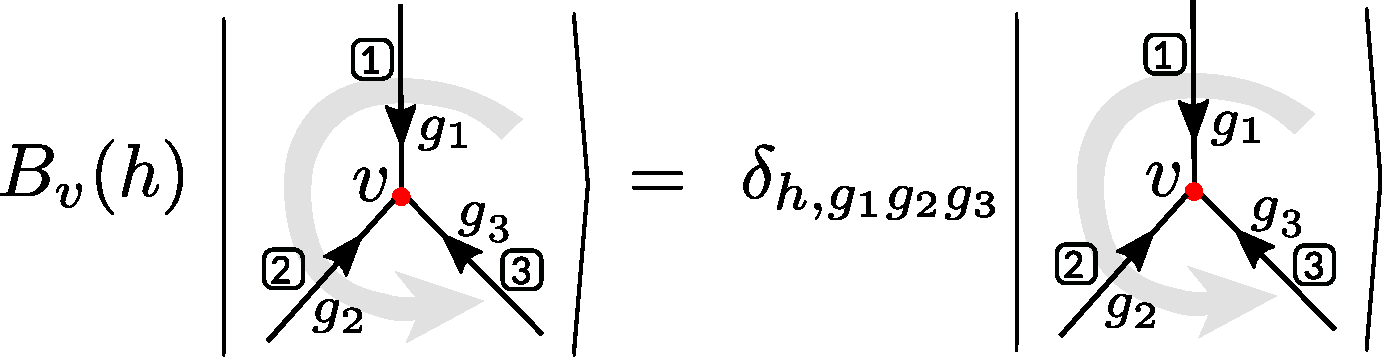
\includegraphics[width= \linewidth]{Figures/B_ops.pdf}
        \caption{Vertex operator. The vertices are oriented in accordance with the plaquette operators (counter-clockwise) and have a starting edge to make the group multiplication assignment unambiguous.}
        \label{eqn:Bs_def}
    \end{subfigure}\hfill
    \begin{subfigure}[b]{0.45\textwidth}
        \centering
        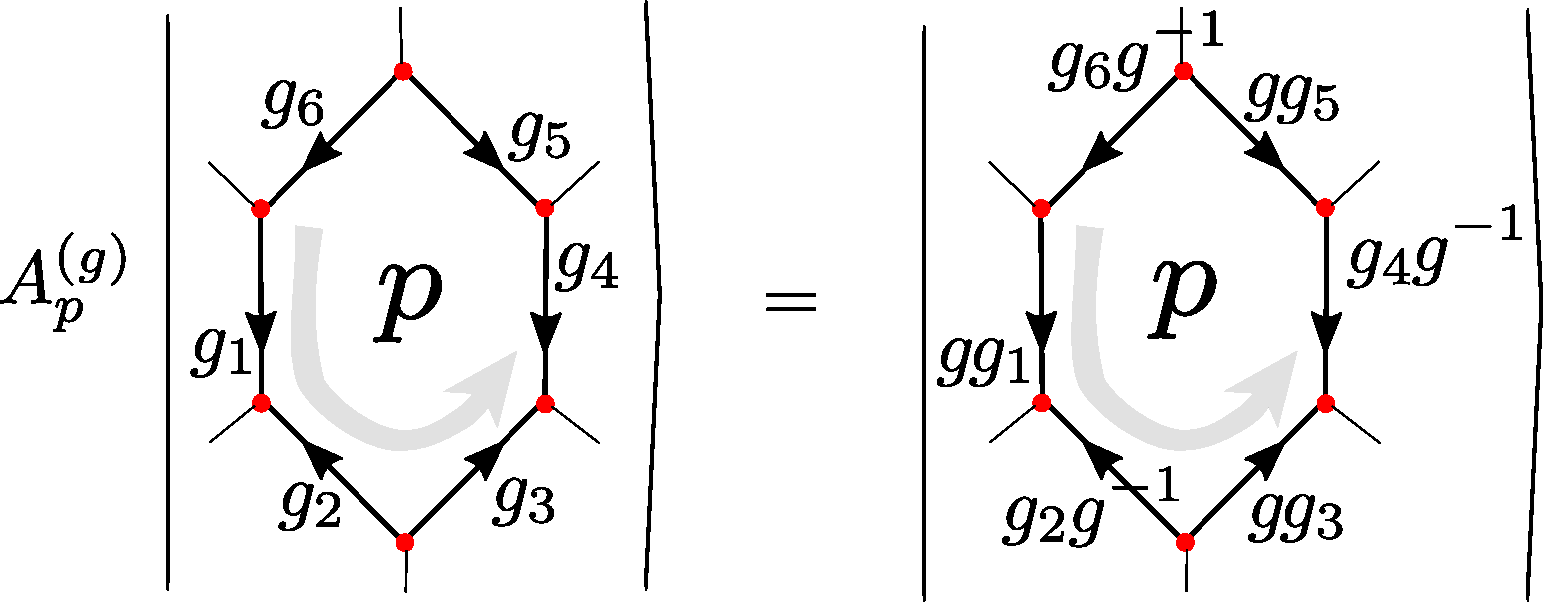
\includegraphics[width = \linewidth]{Figures/A_ops.pdf}
        \caption{Plaquette operator. The orientation of the plaquettes determines pre or post multiplication with the inverse and is chosen in agreement with the orientation of the vertex operators (counter-clockwise).}
        \label{eqn:As_def}
    \end{subfigure}\hfill
    \caption{The vertex and plaquette operators. \caro{todo: figure does not need a,b, and global caption}}
    \label{fig:vertex_ops}
\end{figure*}

\textbf{Ground state.}
It is not hard to verify that all terms in the Hamiltonian commute, Hence we can diagonalize it term-by-term. One can show that the leftover degeneracy depends only on the genus of the surface the graph is embedded in\cite{Kitaev_2003, cui2018topological}. However, we will work on a sphere-topology, where the ground state is unique.

% Used to be a Subsection "Ground State"

%The form of the ground state depends heavily on the geometry of the graph the theory is defined on.
%As an example, ground state degeneracy depends on the topology of the manifold the graph is embedded in.

All terms in the Hamiltonian are also projectors. Hence, one way to construct the ground state is to apply all projectors onto a state that has non-zero overlap with the ground state. In particular, we can start with the state $\ket{\{e\}}$, where every edge is labelled by the identity element.
This state trivially obeys all vertex projectors, so we just need to apply all plaquette projectors
\begin{equation}
    \ket{\psi} = \prod_{p \in P} \mathbf A_p \ket{\{e\}}.
\end{equation}
This state is the unique ground state and corresponds to the equal weight superposition of all states respecting Gauss' law.


% Used to be a Subsection "Excitatons"


%\caro{Move this to GS section}: I do not agree that's better


\subsection{Anyon content}\label{sec:anyon}
In the following we will discuss the anyonic excitations in quantum double models and the algebra describing the latter.

\textbf{The algebra $D(G)$.} The ground state is stabilized\footnote{Meaning, it is the $+1$ eigenstate.} by the projectors in Eq.~\eqref{eqn:ham}. Together with the property $A_p^{(g_1)}A_p^{(g_2)} = A_p^{(g_1 g_2)}$ this implies the stronger condition
\begin{equation}
\begin{split}
    A^{(g)}_p \ket{\psi} = \ket{\psi},\\
    B^{(e)}_v \ket{\psi} = \ket{\psi},
\end{split}\label{eqn:ground_state}
\end{equation}
for all $v \in V$, $p \in P$ and $g \in G$. Therefore, the elementary excitation above the ground state will violate one or more of the equations above and are characterized by how the operators $B_v(h)$ and $A_p(g)$ act on them. More precisely, these operators form an algebra\cite{cui2018topological, Kitaev_2003} (the quantum double algebra $D(G)$), which contains the full information about the anyonic excitations. In particular its irreducible representations label the anyons.

For the toric code model, the $A$ and $B$ operators always commute and their algebras can be investigated independently. One finds the well-known $e$ (for electric) and $m$ (for magnetic) particles associated to vertex and plaquette violations, respectively, and their combination, the fermionic $(e,m)$-particle. However, for non-abelian gauge-groups the operators $A_p(g)$ and $B_v(g)$ whose plaquette and vertex overlap, do no longer commute. To discuss their joint algebra, we consider \emph{sites}
%\footnote{Either some vertices or some plaquettes will be left over depending on the exact geometry of the lattice.} 
 $s_i = (v_i, p_i)$ of adjacent vertices and plaquettes.
%
%\jovan{Soften the approach to formalism by the example of Toric code excitations.}
%%
%Site being occupied by an excitation means that at least one of the conditions in Eq.~\eqref{eqn:ground_state} for that site is violated. In the example of the toric code, $G = \mathbb{Z}_2 = \{0, 1\}$, we have three kinds of excitations. 
%
%These are electric, magnetic and fermionic excitations. The state with an electric excitation at a site $s$ is odd under the action of $A_s^{(1)}$, but is fixed by $B_s^{(0)}$. The state with a magnetic excitation at a site $s$ is annihilated by $B_s^{(0)}$, but fixed under both $A_s^{(g)}$ and by $B_s^{(1)}$. Finally, the state with the fermion at a site $s$ breaks both $A$- and $B$-type conditions, in fact, it is just an electric and a magnetic excitation populating the plaquette and vertex of the site respectively.

%
%In the case of Non-abelian gauge groups, this notion of breaking an $A$-type or a $B$-type condition becomes much more involved due to the more complicated operator algebra being induced by the more complicated group multiplication.
 
Operators on different sites commute trivially, while on the same site we have\footnote{We remark, that the algebraic relations in Eq.~\eqref{eqn:alg} do not depend on the exact grouping of plaquettes and vertices into sites.} 
\begin{equation}
    \begin{split}
        A_s^{(g)}A_s^{(h)} = A_s^{(gh)}, \\
        B_s^{(g)}B_s^{(h)} = \delta_{g,h} B_s^{(h)},\\
        A_s^{(g)}B_s^{(h)} = B_s^{(ghg^{-1})}A_s^{(g)}.
    \end{split}\label{eqn:alg}
\end{equation}
This is the on-site representation of the quantum double algebra $D(G)$ 
\cite{cui2018topological, Kitaev_2003}. 

%In particular, the ground state is the state with the trivial (charge free) representation on each site.
%
%In the case of the toric code, the operator algebra is small, four dimensional, and commutative. It has only four irreducible representations, which we mentioned above: vacuum, electric, magnetic and fermionic.
 
%\caro{At some point we need to introduce the notion of pure charge, pure flux and a dyon, we should state the simplified expressions for pure charge and pure flux, and the notion of generalized conjugation in the dyon case, as we use this later on.}

We will now discuss its irreducible representations. However, we will refrain from providing any derivations (see e.g. Ref.~\cite{Cui_2015}) and just state the results. 

The irreducible representations are labelled by two objects, a conjugacy class $C$ of the group $G$ and an irreducible representation $\chi$ of the centralizer, $Z(r)$, of the class representative $r \in C$. The vector space on which $(C, \chi)$ acts is spanned by a basis $\ket{\mu} = \ket{c, i}$, where $c \in C$ and $i \in \{1, 2, \ldots, \text{dim}\chi\}$, i.e. the first index goes over the conjugacy class elements while the second goes over the vector indices of the irreducible representation $\chi$.

Note, that in the case of abelian groups, in particular the toric code, the conjugacy classes are trivial and identical to the group elements themselves. Their center is $G$, which has $|G|$ one-dimensional representations. Hence, the irreducible representations factorize as indicated above. 

In the general, non-abelian case the irreducible representations do not factorize as can be seen from the action of the algebra generators on the vector space spanned by $\ket{\mu}=\ket{c,i}$ %\caro{what happens with $i,i'$ in the first line?} 
%\begin{equation}
%    \begin{split}
%        B^{(h)}_{\mu\nu}=\bra{c, i} B^{(h)} \ket{c', i'} = \delta_{c, h} \delta_{c, c'}\delta_{i, i'}, \\
%        A^{(g)}_{\mu\nu} = \bra{c, i} A^{(g)} \ket{c', i'} = \delta_{c,gc'g^{-1}} \Gamma^\chi_{ii'}(q_{c}^{-1}gq_{c'}),
%    \end{split}
%\end{equation}
\begin{equation}
    \begin{split}
        B^{(h)}_{\mu\nu}=\bra{c, i} B^{(h)} \ket{c', i'} = \delta_{c, h} \delta_{c, c'}\delta_{i, i'}, \\
        A^{(g)}_{\mu\nu} = \bra{c, i} A^{(g)} \ket{c', i'} = \delta_{c,gc'g^{-1}} \Gamma^\chi_{c,ii'}(g),
    \end{split}
\end{equation}
where $\Gamma^\chi_c(g)$ are the $\chi$-representation matrices. The latter are defined for elements of the centraliser $Z$ which are obtained from $g$ via the map $q_{c}^{-1}gq_{c'}$, where $q_c$ is a group element that satisfies $q_c c q_c^{-1} = r$ and $c'=g^{-1}cg$. 
%\caro{omit: These representation matrices are going to play a central role in our protocols for creating and manipulating anyons.}


To get a better understanding of the meaning behind these expressions, we consider three simple examples. Let us start with the vacuum (or trivial) representation, labelled by $(\{e\}, \mathbb{1})$. This representation is one-dimensional and spanned by $\ket{e, 0}$
\begin{equation}
    \begin{split}
        B^{(h)}\ket{e, 0} = \delta_{h,e}\ket{e, 0},\\
        A^{(g)}\ket{e, 0} = \ket{e,0}.
    \end{split}
\end{equation}
Hence, Eq.~\eqref{eqn:ground_state} implies that for the ground state every site houses the trivial representation.

Other important examples are pure charges and pure fluxes. A pure flux is labelled by a conjugacy class and the trivial representation of its centre, $(C, \mathbb{1})$. Its basis vectors are $\ket{c, 0}$ for $c \in C$, with
\begin{equation}
    \begin{split}
        B^{(h)}_{\mu\nu}=\bra{c, 0} B^{(h)} \ket{c', 0} = \delta_{c, h} \delta_{c, c'}, \\
        A^{(g)}_{\mu\nu} = \bra{c, 0} A^{(g)} \ket{c', 0} = \delta_{c,gc'g^{-1}}.
    \end{split}
\end{equation}
Pure flux excitations only violate the vertex term, the $B$-term.

Pure charge excitations are labelled by the group identity and a representation of the group $G$ itself, $(\{e\}, \chi)$. Its basis vectors are $\ket{e, i}$ for $i \in \{1, 2, \ldots, \text{dim}\chi\}$, with
\begin{equation}
    \begin{split}
        B^{(h)}_{\mu\nu}=\bra{e, i} B^{(h)} \ket{e, i'} = \delta_{e, h},\\
        A^{(g)}_{\mu\nu} = \bra{e, i} A^{(g)} \ket{e, i'} = \Gamma^\chi_{ii'}(g).
    \end{split}
\end{equation}
Pure charge excitations only violate the plaquette term, the $A$-term.


In particular, if we have a gauge field state, $\ket{\chi, p; i}$, where each site houses a trivial representation except for one, $(v, p)$, which is occupied by a pure charge $(\{e\}, \chi)$, this state satisfies all the constraints in Eq.~\eqref{eqn:ground_state} except for
\begin{equation}
    A_p^{(g)}\ket{\chi, p; i} = \sum_{i'} \Gamma^\chi_{ii'}(g)\ket{\chi, p; i'},\label{eqn:tranfs}
\end{equation}
where $i$ and $i'$ are the internal degrees of freedom of the charge\footnote{Note that the charge can be vector valued for non-abelian symmetry groups.}.
This is the way a charged state transforms under gauge transformations in gauge field theory. Hence, we say that the plaquette terms generate gauge transformations.

All other excitations are called dyons. They violate vertex and plaquette terms simultaneously, meaning they have a flux component associated with a vertex of the site $(v,p)$ and a charge component associated with its plaquette, but unlike the toric code fermion cannot be broken down to a combination of pure charge and pure flux sitting next to one another.

\textbf{Non-abelian anyons} To understand the distinction between abelian and non-abelian anyons we will focus on the physical meaning of the dimension $d = \text{dim}(C, \chi) = |C|\text{dim}(\chi)$ of the irreducible representations.

If we have a gauge field state with an anyon of type $(C, \chi)$ at a site $s$, the plaquette and vertex terms of that site will transform this state in accordance with that algebra representation. This implies that specifying the type and location of this anyon does not uniquely fix the gauge field state. Instead, there is a $d$-dimensional subspace $\mathcal H_s(C,\chi)$ of the total Hilbert space associated with this anyon occupying this site. This $d$-fold degeneracy can be interpreted as a spin-like internal degree of freedom of the anyon.

Generalising this, we find that for a state with specified charge content $\{(C_s, \chi_s)\}_s$ on all sites $s$ the subspace associated to this configuration is
\begin{equation}
	\mathcal{H}_{\{s\}} = \bigotimes_s \mathcal H_s (C_s, \chi_s).
\end{equation}

A more powerful alternative to this local description can be derived if we notice that
there is an algebra associated with the tensor product of representations, analogous to the Clebsch-Gordan (CG) decomposition of tensor products of linear representations of a group into the direct sum of irreducible representations. 

In particular, if we have two charges $a$ and $b$ the assiociated Hilbert space can be written as a direct sum of the Hilbert space associated to charges $c$. We write this as 
\begin{equation}
	a \otimes b = \bigoplus_{c}N^c_{ab} c,\label{eqn:fuse} 
\end{equation}
with $a$, $b$ and $c$ going over a set of anyon labels $(C, \chi)$ and $N_{ab}^c$ being integer coefficients. 


%\begin{equation}
%\begin{split}
%	(\{e\}, \chi_i)\otimes (\{e\}, \chi_j) = \bigoplus_k n^k_{ij} (\{e\}, \chi_k) \;,	
%\end{split}
%\end{equation}
%where .

How this manifests physically is that if we have two anyons $a$ and $b$ in some region and measure the topological charge associated to that region we may get any label $c$ for which $N_{ab}^c \neq 0$. This process is referred to as anyon fusion.

While the general expression for the $N_{ab}^c$ is cumbersome and can be found in Appendix \ref{app:fusion}, for pure charge anyons $(\{e\}, \chi_i)$ it readily reduces to the well-known  decomposition of tensors products of group irreps into direct sums of irreps $\chi_i\otimes\chi_j = \bigoplus_k n^k_{ij} \chi_k$.

If the gauge group is abelian all algebra representations are one-dimensional and there is no degeneracy once the charge content of a gauge field is specified. The fusion is unambiguous. 
We can see that by looking at the dimensions of the LHS and RHS of Eq.~\eqref{eqn:fuse}. For every $a$ and $b$ there is only one $c$ for which $N_{ab}^c$ is nonzero, i.e. one.

The Hilbert space associated with the presence of multiple non-abelian anyons is the stage on which all striking phenomena of non-abelianess are played out. Besides the possibility of multiple fusion outcomes discussed above,  also moving anyons around one another (braiding) acts non-trivially on this space and corresponds to a unitary operation. In such a braiding process the order of exchanges matter as in general the unitary matrices associated to the individual exchanges do not commute. The full theory that describes the braiding and fusion of anyons is a so-called unitary modular tensor category (UMTC)\cite{Kitaev_2003} and the UMTC for the anyons of quantum double models is reviewed in Appendix \ref{app:umtc}.

%
%As an example, let us take the charge content of the gauge field to be four Non-abelian anyons of the same type $a$ occupying four sites and look at the form of the degenerate subspace $\mathcal H_{\text{deg.}}$.
%Using the algebra of Eq.~\eqref{eqn:fuse} to simplify the form of the subspace we get 
%\begin{equation}
%	\mathcal{H}_{\text{deg.}} = \bigoplus_{c, d, f} N_{aa}^c N_{ca}^d N_{da}^ff,\label{eqn:decomp} 
%\end{equation}
%also assuming that we have measured zero total topological charge of the four sites, i.e. $f$ is fixed to be $(\{e\}, \mathbb{1}) = 0$.
%
%The space has $D = \sum_{c, d, f} N_{aa}^c N_{ca}^d N_{da}^0$ one-dimensional sectors, each spanned by the one vector in the trivial representation, $\ket{e,0}$. The sector are labeled by the fusion outcomes $(c, d)$ for which none of the algebra coefficients vanish. Therefore, this space is also called the fusion space and a its natural basis the fusion tree basis
%$$\mathcal{H}_{\text{deg.}} = \mathcal{H}_{\text{fusion}} = \text{span}_{(c,d)}\{\ket{c,d; e, 0}\}.$$
%
%Note that this description has nothing to do with the local spin-like variables we began with and is completely determined by the fusion algebra.
%
%Also note that addition of sites occupied by the vacuum doesn't change anything since vacuum fuses trivially with other representations, $a\otimes0 = a$.
%
%\jovan{assumed def in the intro}
%Finally, to answer why studying the space $\mathcal{H}_{\text{fusion}}$ is important in the first place, we look at the action of \emph{anyon braiding}. Braiding doesn't change the charge content, hence, it must transform states only within this degenerate space. Therefore, the degeneracy must be non-trivial, i.e. anyons Non-abelian for their braiding to have any computational power. 
%
%The braiding action is best described in the global fusion tree basis in terms of topological variables such as the $F$- and $R$-symbols \cite{cui2018topological, Kitaev_2003}. See Appendix \ref{app:braid} for the treatment of braiding of quantum double anyons in both local spin-like and fusion tree basis. \jovan{Needs reform.}
%
%
\subsection{Ribbon Operators}\label{sec:ribbon_ops}

In the following, we will explain how to create and move anyons. Anyons are always created in pairs from the vacuum. 
%
%To see why, imagine we take the ground state on a 2-sphere, the state is a superposition of all assignments of group elements to edges that do not violate the Gauss' law. Now we shift the label of one of the edges, $e_0$, by some constant group element. The superposition is now made up from different assignments, which only differ on the edge $e_0$. This action disturbs two vertex operators on each end of the edge $e_0$, i.e. a pair of pure fluxes have been created.
%
%Analogously, there are operations on the edge $e_0$ that disturbs two plaquette operators touching the edge $e_0$. i.e. that create a pair of pure charges.
%
%Moreover, 
For any anyon, $(C, \chi)$, and any path in the graph between two sites, see Figure \ref{fig:rib_exampl}, there is a \emph{ribbon operator} that creates a pair of said anyons at the end sites. 
%These paths are called ribbons and the associated operators ribbon operators, which themselves are labelled by the anyons they create, $(C, \chi)$.

If the ribbons are closed and contractable, the associated ribbon operators leave the ground state unchanged. Moreover, they span the loop operator algebra that leave the ground state invariant. It is in that way that the quantum double ground state knows about the anyon spectrum.

We will not explain the derivation of the ribbon operators themselves, see Ref \cite{Kitaev_2003,cui2018topological}, just how to apply them to a state.
%
\jovan{General, add to introduction: These operators represent a planar diagram algebra, i.e. a braiding group representation generated by a specific Braiding Tensor Category (BTC) and hence were conceived as a model of a system that can perform fault-tolerant quantum computing by the means of braiding anyons.
However, even though the braid group itself is universal its image on this planar diagram algebra is finite, hence non-universal \cite{cui2018topological}. For some gauge groups it can be made universal by the addition of measurements \cite{Cui_2015}.}
%
The ribbon operators are not unitary in general. If the anyons have a dimension larger than one, the operators that create and manipulate them are non-local projectors. To simulate them on a digital quantum computer requires ancillas and measurements. 

\caro{%skip or turn footnote 
In Ref. \cite{andersen2022observation} the group overcame this issue by means of unitary lattice deformations, unitarily transforming from a state with a set of non-abelian anyons on one graph to another state with the same anyon content but defined on a different graph, hence they were able to move the Non-abelian Majorana fermions unitarily. However, these are extrinsic and static lattice defects on top of a theory that is an abelian $\mathbb Z_2$ gauge theory, hence, the nature of their non-abelian anyons is different from intrinsic gauge field excitations.}

%\subsubsection{Application Scheme}


%Say we have a ribbon of type $(C, \chi)$ whose anyons have dimension $d = \text{dim}(C, \chi)$.

As we mentioned, the pair of $d$-dimensional anyons define a $d^2$-dimensional degenerate subspace of the gauge field Hilbert space that encodes the outcomes of their fusion. This encoding is increasingly non-local as we separate the anyons, this being the main idea of topological quantum computation with anyons. We, however, require accessing this information locally to move the anyons. To this end, we keep one auxiliary qudit per end of the ribbon.

Every ribbon (cf. Fig.~\ref{fig:rib_exampl}) is made up from two types of elementary triangles
\begin{itemize}
    \item[I)] A triangle consisting of two vertices and one plaquette center. One side coincides with an edge of the graph.
        \item[II)] A triangle consisting of two plaquette centers and one vertex. One of the triangle's sides crosses an edge of the graph.
%    \item[I)] Triangles whose side follow the edge they touch, whose points include two vertices and one plaquette. These triangles move the flux component of the anyon from the first vertex to the second vertex,
%    \item[II)] Triangles which cross the edge they touch, whose points include two plaquettes and one vertex. these triangles move the charge component of the anyon from the first plaquette to the second plaquette.
\end{itemize}
Moving anyons means appending elementary triangles onto a ribbon. Each triangle type corresponds to a specific operator, the details of which also depend on the orientations of the edges and whether the triangle is attached to the back or front end of the ribbon. A detailed list is provided in Fig.~\ref{fig:all_triang} in Appendix \ref{app:ribs}.


\begin{figure}
    \centering
    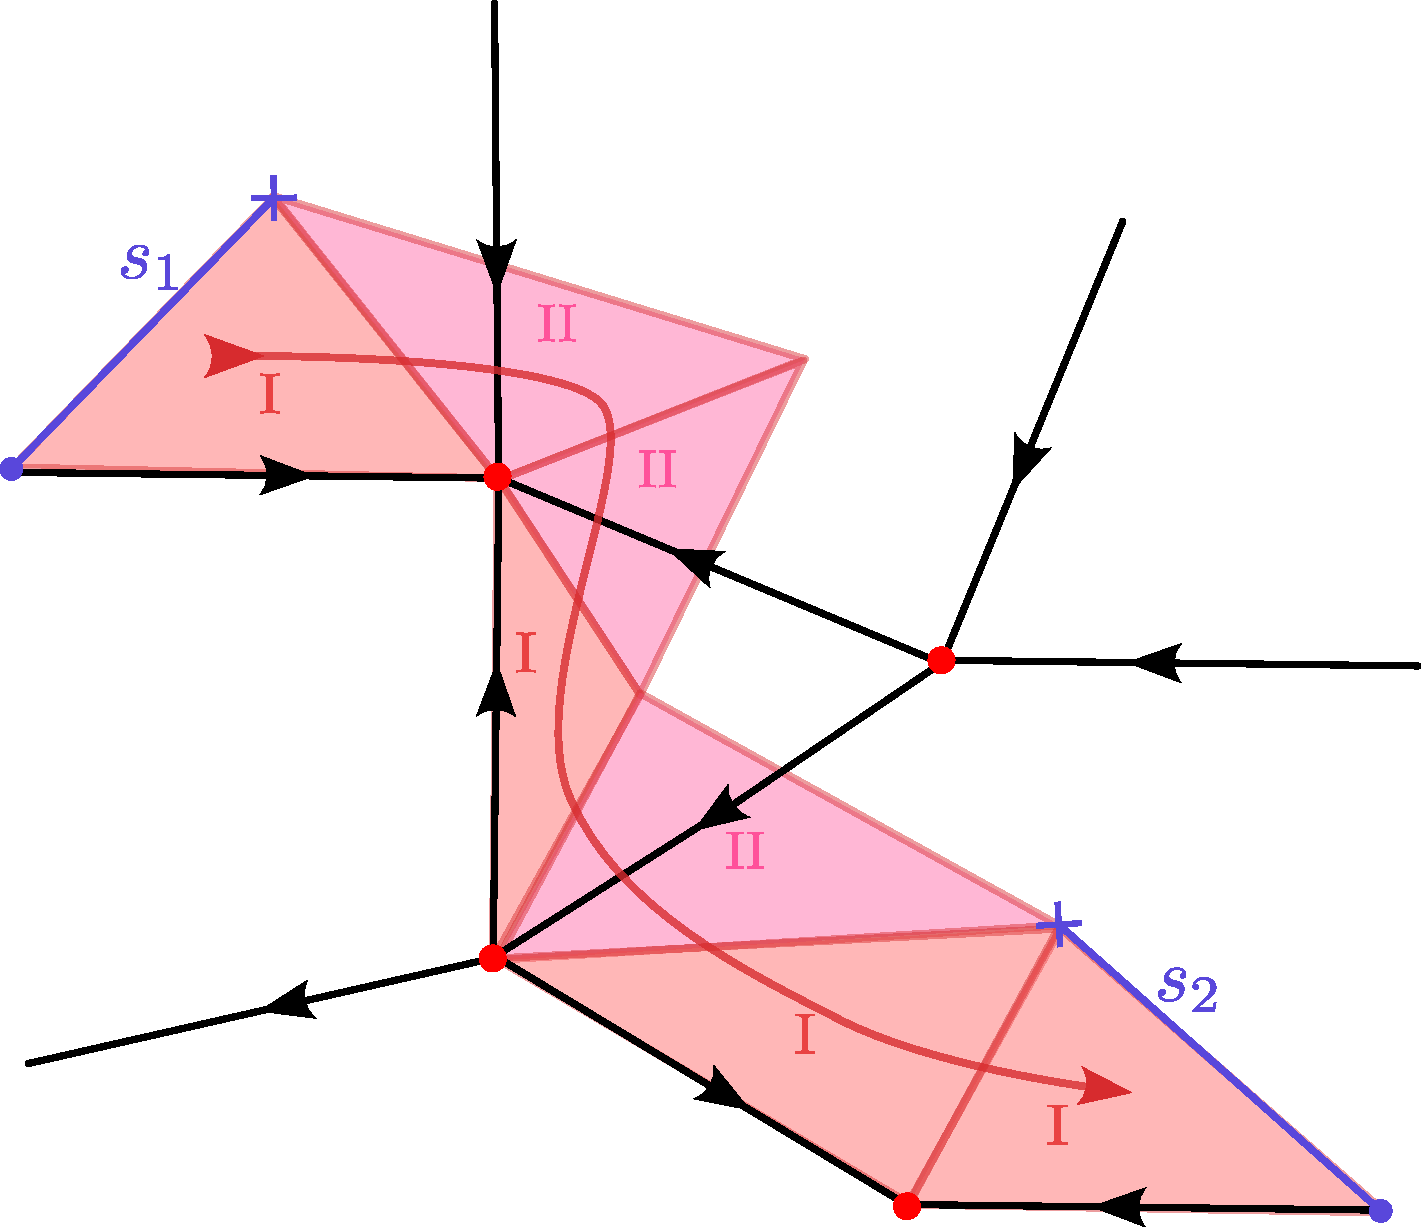
\includegraphics[width= \linewidth]{Figures/ribbon_exampl.pdf}
    \caption{An example of a ribbon, $R = \{t_1, t_2, \ldots, t_7\}$, between site $s_1$ and $s_2$. The ribbon is made up from four Type I elementary triangles and three Type II elementary triangles, they are labelled.}
    \label{fig:rib_exampl}
\end{figure}


%\caro{You do that sequentially, i.e., not just 'for all $t_i$' but one after another. Also, would be easier to just talk about a forward moving ribbon where you only have $|c,i\rangle$ and $|g\rangle$ and then consider backwards in an appendix} I would still include both qubits, since there are two indices in the def. of F


%\textbf{The algorithm} that creates two anyons along a ribbon path $R$ made up from a set of triangles $R = \{t_1, t_2, \ldots, t_N\}$ in the internal state: $\ket{\alpha; \beta} = \ket{c', i'; c, i}$ i.e. applying $F_{\alpha, \beta}^{(C,\chi)}(R)$ is:\begin{enumerate}
%    \item Initialize the two auxiliary qudits in the states $\ket{\alpha, \beta}$. We will think of the first qudit as the ribbon's backend and the second as its frontend.
%    \item In the case of growing the ribbon from $t_1$ onwards, for each $t_i$ sequentially in R do one of the following unitaries depending on the \textit{Type} (and orientation) of the triangle $t_i$: \begin{itemize}
%        \item[I)] Multiply the label of the $t_i$'s edge by the group element encoded by the forward auxiliary qudit: $\ket{c', i';c, i}\ket{g}_{t_i} \rightarrow \ket{c', i';c, i}\ket{cg}_{t_i}$.
%        \item[II)] (Generalize-)Conjugate the forward axially qudit by the label of the edge crossed by $t_i$: $\ket{\alpha;\beta}\ket{g}_{t_i} \rightarrow \sum_\gamma A_{\gamma\beta}^{(g)}\ket{\alpha;\gamma}\ket{g}_{t_i}$.
%    \end{itemize}
%    \item Project the ancillary qudits to a Bell-pair state: $\bra{\Phi^+} = \frac{1}{\sqrt{d}}\sum_\nu \bra{\nu; \nu}$.
%\end{enumerate}



\textbf{The algorithm} that creates two anyons of type $(C,\chi)$ along a ribbon path $R$ in the internal state $\ket{\alpha; \beta} = \ket{c', i'; c, i}$ is the following
\begin{enumerate}
    \item Initialise two auxiliary qudits in the states $\ket{\alpha; \beta} = \ket{c', i'; c, i}$  We will think of the first qudit as the ribbon's back end and the second as its front end.
    \item For each triangle in the ribbon, sequentially apply one of the following unitaries depending on the triangle \textit{type} (and the edge orientations) 
    \begin{itemize}
        \item[I)] Multiply on the coincidng edge\\  $\ket{c, i}\ket{g}_\text{phys} \rightarrow \ket{c, i}\ket{cg}_\text{phys}$.
       \item[II)] Generalised-conjugate by the crossed edge\\ $\ket{c,i}\ket{h}_\text{phys} \rightarrow \ket{gcg^{-1}} \Gamma^\chi_c(h) \ket{i} \ket{h}_\text{phys}$.
    \end{itemize}
    \item Project the ancillary qudits to the Bell state $\bra{\Phi^+} = \frac{1}{\sqrt{d}}\sum_\nu \bra{\nu; \nu}$. The projection is done by measurement and post-selection.
\end{enumerate}
For the other variants of step 2, for different edge orientations etc., consult the Figure \ref{fig:all_triang} in Appendix \ref{app:ribs}. 

In the way presented above, we have started building up the ribbon from start-to-finish using only forward-type elementary triangles. Similarly, we could have started in the middle and extend in parallel both forward and backwards with appropriate types of elementary triangles, see Appendix \ref{app:ribs}. Backwards-type elementary triangles, analogously to Step \textbf{2.} stated above, act with the backwards auxiliary qudit.

As we can see the operation is sequential so at best the depth of a circuit implementing this is $\mathcal{O}(|R|)$, with the best depth achieved by starting at the middle and growing it both ways.

Of course, we can make this constant depth by separating the main ribbon into $|R|$ smaller ribbons which however requires $|R|$ pairs of qudits. To merge these ribbons, we also need $|R|$ Bell-pair projections. As these are done via measurement and post-selection this requires an exponential in $|R|$ number of repetitions for a $\mathcal{O}(1)$ number of successful projections.

To interpret what we have here, let us look at the quantum resources. We have the qudits representing the matter $\mathcal{H}_{\text{matter}}$ and the ancillary bits representing the internal state of the anyons, or the fusion space, $\mathcal{H}_{\text{ancilas}} \equiv \mathcal{H}_{\text{fusion}}$ which is already embedded non-locally in  $\mathcal{H}_{\text{matter}}$.

The two types of triangles couple the two spaces in two different ways, for type I the $\mathcal{H}_{\text{ancilas}}$ controls an action on $\mathcal{H}_{\text{matter}}$ and for type II it is the other way around. After the measurement that disentangles, the redundant copy of $\mathcal{H}_{\text{fusion}}$ the $\mathcal{H}_{\text{matter}}$ is left in a state with the ribbon operator imprinted on it as signalled by the topological charge, braiding amplitude and phase.

%\jovan{add something about the non-commutativity of these operations and their action on the degen. space}

\subsection{Charge Measurements}
%\caro{Explain the idea of reduced charge measurement in words, i.e., get partial information and combine the partial information for different $H$ to deduce charge}

In this section, we will explain how we measure the topological charge, i.e., the anyon label. This is the last element of our toolkit for probing topological order. The ideal charge measurement would differentiate any type of excitation on any site, such measurement is associated with the following set of projectors \cite{}:
\begin{equation}
    P_s^{(C, \chi)} = \frac{\chi(e)}{|Z(r)|}\sum_{c \in C}\sum_{z \in Z(r)}\chi^*(z)B_s^{(c)}A_s^{(q_c z \bar{q}_c)},
\end{equation}
for each irreducible representation of the $D(G)$.

Since we work in a basis where projectors onto a given $G$-valued flux through a vertex $v$, $B_v^{(h)}$, are diagonal, we can just do a full projective measurement of the gauge field degrees of freedom in that basis. 
The result of such measurement is a labelling of all edges by group elements from which we can compute the flux through any vertex. 

However, in order to measure the charge component, one needs to implement a controlled $A^{(g)}_s$ operator which needs a controlled group multiplication applied to all edges of $s$'s plaquette, i.e. $\ket{g}\ket{g_i} \rightarrow \ket{g}\ket{gg_i}$ for all $\ket{g_i}$ around the plaquette.
This requires circuits which, in the case of non-abelian groups such as $D_4$ which we will study in more detail, are prohibitively expensive. 

The main idea to circumvent this problem is to instead use partial charge measurements that have a substantially reduced circuit depth. Such partial measurements do not determine the charge completely. However, when we combine a set of different partial measurements we are able to deduce the full charge content from the measurement outcomes.

% Used to be a subsection: {Reduced Charge Measurement}

%\caro{general comment: just talk about the reduced charge measurement, make the purpose of it clear in the first few sentences: reduced circuit depth is traded for only gaining partial information because measurement outcomes for a single subgroup are compatible with several charges, repeating the measurement for different subgroups allows to deduce charge uniquely for examples considered (D4, Q8), skip all of the following until}

The key idea behind the partial measurement protocol is that controlled $A_s^{(g)}$ becomes significantly simpler to perform once we restrict ourselves to a proper subset of the full group, i.e. $g \in H \subset G$.

With Eq.~\eqref{eqn:tranfs} in mind, we propose the following algorithm for the $H$-reduced charge measurement on a plaquette $p$:\begin{enumerate}
    \item Prepare an auxiliary qudit, $a$, encoding the elements of $H\subset G$, in an equal superposition over all elements, so that the joint total state of the system is: $$ \sum_{h \in H} \ket{h}_a\ket{\psi}_\text{phys}. $$
    \item Apply a $a$-controlled $A$-multiplication onto the edges of the plaquette $p$$$ \sum_{h \in H} \ket{h}_a\ket{\psi}_\text{phys} \rightarrow \sum_{h \in H} \ket{h}_a A^{(h)}_p \ket{\psi}_\text{phys}. $$
    \item Apply a unitary $$ U_a = \sum_{\chi_H}\sum_{i', j'}\sum_{h'\in H}  \Gamma^{\chi_H}_{i'j'}(h')  \ket{\chi_H; i', j'}_a\bra{h'}_a $$ onto the auxiliary qudit $a$. Here the $\chi_H$ labels the irreducible representations of $H \subset G$, $\Gamma^{\chi_H}(h')$ are the representation matrices, with $i'$ and $j'$ being the vector indices for a given representation $\chi_H$.
    \item Measure the auxiliary qudit $a$.
\end{enumerate}

%Needs a case example
To see how this protocol works, let us examine the case of a  gauge field with well-defined pure charge on a plaquette  $\ket{\psi}_\text{phys} = \ket{\chi; i}$. Using  Eq.~\eqref{eqn:tranfs} we can write the joint state after step 2 as
\begin{equation}
    \sum_{h \in H} \ket{h}_a A^{(h)}_p \ket{\chi; i} = \sum_{h \in H} \ket{h}_a \Gamma^{\chi}_{ij}(h) \ket{\chi; j}.
\end{equation}

If $H = G$, the state after step 3 becomes\begin{equation}
    \begin{split}
        \sum_{h \in G} U_a\ket{h}_a \Gamma^{\chi}_{ij}(h) \ket{\chi, p; j} = \\
        \sum_{h \in G} \sum_{\chi'}\sum_{i', j'}  \Gamma^{\chi'}_{i'j'}(h)\Gamma^{\chi}_{ij}(h) \ket{\chi'; i', j'}_a \ket{\chi, p; j} =\\
        \sum_j\ket{\chi; i, j}_a \ket{\chi, p; j}
    \end{split}
\end{equation}
The decoupling we see in the last line after summing over $h$ is guaranteed by Schur's orthogonality lemma.

In the case above, the result of the measurement in step 4 is a label $(\chi, i, j)$, representing the charge, the internal state before the measurement and the internal state after the measurement.

If we, however, take $H \subset G$, then the charge information is partial.
By partial charge information, we mean that the result of the measurement in the last step, the label $(\chi_H, i, j)$ is no longer compatible with only one charge but a set of charges, i.e. the charge is not fully determined.

We may repeat the procedure using different subsets $H \in G$ to gather further partial information on the charge in the hope that we will be able to deduce the charge fully. In the considered examples, choosing different subgroups proves to be sufficient. This relies on the partial orthogonality of character tables of a group and its subgroup, and is demonstrated for the example of the group $D_4$ below.

\subsection{Quantum Double of $D_4$}

Throughout the rest of the paper we will focus on the group $D_4$ and its lattice gauge theory.
Hence in this section, we will describe the group structure of $D_4$, its quantum double algebra, as well as representation theory of both.

The dihedral group of order 8 is the symmetry group of a square. It is generated by a $\pi/2$-rotation $r$ and a reflection  $m$ along a diagonal.
The group law is defined by following identities
\begin{equation}
	\begin{split}
		r^4 = e,\;
		m^2 = e,	\;	mr = r^3m. \label{eqn:group}
	\end{split}
\end{equation}

This group is solvable and all of its proper subgroups are abelian. It can be decomposed as $D_4 = \mathbb{Z}^m_2 \ltimes \mathbb{Z}^r_4$.
This decomposition is not unique, $D_4 = \mathbb{Z}_2^m\ltimes(\mathbb{Z}_2^{r^2}\times\mathbb{Z}^{mr}_2)$ is also a valid decomposition.\footnote{The superscripts in $\mathbb{Z}_n^x$ label the group generator.}
%, $\mathbb{Z}_n^x = \{x, x^2, \ldots, x^{n-1}, x^n = e\}$.}

The conjugacy classes of $D_4$ alongside their centres are listed in Table \ref{tab:conjs}.
\begin{table}[h]
\centering    \begin{tabular}{|c | c|}\hline
         $C$ & $Z(r) \text{, } r\in C$\\ \hline $\mathcal C_e = \{e\}$ & $D_4$\\ $\mathcal C_{r^2}= \{r^2\}$ & $D_4$\\ $\mathcal C_{r}=\{r, r^3\}$ & $\mathbb{Z}_4^r \equiv H_r$\\ $\mathcal C_m=\{m, mr^2\}$& $\mathbb{Z}_2^m \times \mathbb{Z}_2^{r^2}\equiv H_m$ \\ $\mathcal C_{mr}=\{mr, mr^3\}$& $\mathbb{Z}_2^{mr} \times \mathbb{Z}_2^{r^2}\equiv H_{mr}$\\
         \hline 
    \end{tabular}
    \caption{The conjugacy classes of $D_4$ alongside their centres.}\label{tab:conjs}
\end{table}
There are five conjugacy classes, which implies that there are also five irreducible representations. Their dimensions are $(1,1,1,1,2)$. The characters, i.e., the traces of the representation matrices, are given in Table \ref{tab:char}.
\begin{table}[h]
\centering    \begin{tabular}{|c|c c c c c |}
         \hline
         $D_4$ & $\mathcal C_e$ & $\mathcal C_{r^2}$ & $\mathcal C_{r}$ & $\mathcal C_m$ & $\mathcal C_{mr}$ \\
         \hline
         $1$ & 1 & 1 & 1 & 1 & 1 \\
        % \hline
         $\alpha_r $& 1 & 1 & 1 & -1 & -1  \\
         %\hline
         $\alpha_{m}$ & 1 & 1 & -1 & 1 & -1  \\
         %\hline
         $\alpha_{mr}$ & 1 & 1 & -1 & -1 & 1  \\
         %\hline
         $\epsilon$ & 2 & -2 & 0 & 0 & 0  \\
         \hline 
    \end{tabular}
    \caption{Character table of $D_4$.}\label{tab:char}
\end{table}

When labelling the representations of the algebra $D(D_4)$ we will also need the irreducible representations of the centres of the conjugacy classes. The centres of the three non-trivial conjugacy classes are abelian and have four elements. Hence, they have four one-dimensional irreducible representations. Their character tables are shown in Table~\ref{tab:char_sub}.
\begin{table}[h]
\centering
\begin{tabular}{|l|llll|}\hline
  $H_r$ & $e$ & $r$ & $r^2$ & $r^3$ \\ \hline
$1$ & $1$   & $1$            & $1$             & $1$                                  \\ 
$i$ & $1$   & $i$            & $-1$             & $-i$                                  \\ 
$-1$ & $1$   & $-1$            & $1$             & $-1$                                  \\ 
$-i$ & $1$   & $i$            & $-1$             & $i$                                  \\ \hline
\end{tabular}
\begin{tabular}{|l|llll|}\hline
  $H_m (H_{mr})$ & $e$ & $m(mr)$ & $r^2$ & $mr^2(mr^3)$ \\ \hline
$(1,1)$ & $1$   & $1$            & $1$             & $1$                                  \\ 
$(1,-1)$ & $1$   & $-1$            & $1$             & $-1$                                  \\ 
$(-1,1)$ & $1$   & $1$            & $-1$             & $-1$                                  \\ 
$(-1,-1)$ & $1$   & $-1$            & $-1$             & $1$                                  \\ \hline
\end{tabular}
\caption{Character tables of relevant subgroups of $D_4$. The groups $H_m$ and $H_{mr}$ are isomorphic.}
\label{tab:char_sub}
\end{table}

The task of listing all of the irreducible representations of $D(D_4)$ and their dimensions from this data is straightforward. There are $2 \times 5  + 3 \times 4 = 22$ irreducible representations, i.e., types of anyons in the $D_4$ quantum double model.

Eight of them are one-dimensional, i.e. abelian, while the rest are two-dimensional. Other than the vacuum, four of them are pure charges and four are pure fluxes. For dyons with the $\mathcal{C}_{r^2}$ flux component we say that they have a trivial flux. The flux can be factored out, just like in the case of the toric code fermion. This comes from the fact that $r^2$ commutes with all group elements, just like the identity. 

\textbf{Anyon content of $D(D_4)$.} We label the vacuum and the trivial flux as $0 \equiv (\mathcal{C}_e, 1)$ and $\tilde 0 \equiv (\mathcal{C}_{r^2}, 1)$, respectively. Likewise, the pure charges and dyons with trivial flux are labelled as $\Sigma_{\chi} \equiv (\mathcal{C}_e, \chi)$ and $\tilde{\Sigma}_{\chi} \equiv (\mathcal{C}_{r^2}, \chi)$, with $\chi$ being one of the nontrivial irreducible representations of $D_4$.
Nontrivial pure fluxes are labelled $\Psi_x = (\mathcal{C}_x, 1)$, with $C_x$ being one of the nontrivial conjugacy classes of $D_4$. The rest of the dyons have less informative labels such as $\{\tilde{\Psi}_x, \Phi_x, \tilde{\Phi}_x\}$ and can be found in Appendix \ref{app:reps}.

\textbf{Charge Measurements Reprise.}
Let us review the partial charge measurements for $D(D_4)$.
We choose the subgroups $\{H_r, H_m, H_{mr}\}$ for the measurement protocol. All the irreducible representations of these subgroups, $\chi_{H_x}$, are one dimensional, this means that the measurement outcome of the reduced charge measurement is just the irrep label $(\chi_{H_x})$. Looking at their character tables, we note the partial orthogonality with the characters of the irreps of $G$. 

%The character table of $D_4$ is given in Table \ref{tab:char}, while the character tables of relevant subgroups are given in Table \ref{tab:char_sub}. Note, the subgroups $\{H_r, H_m, H_{mr}\}$ were mentioned in the context of centres of relevant conjugacy classes, but they also prove to be a great choice of subgroups to be used in the reduced charge measurement protocol, in this case. \jovan{word better}


More concretely, we compute $ \braket{\chi_{H_x}, \chi} = \sum_{h\in H_x} \chi_{H_x}(h)\chi(h)$ for the five different charges and list the results in Table \ref{tab:red_ch}.


\begin{table}[h]
\centering
\begin{tabular}{l|lllll}
  $\braket{\chi_{H_r}, \chi}$ & $1$ & $\alpha_{r}$ & $\alpha_{m}$ & $\alpha_{mr}$ & $\alpha_{\epsilon}$ \\ \hline
$1$ & 4   & 4            & 0             & 0               & 0                   \\ 
$-1$ & 0   & 0            & 4             & 4               & 0                   \\ 
$i$ & 0   & 0            & 0             & 0               & 4                   \\ 
$-i$ & 0   & 0            & 0             & 0               & 4                   \\ 
\end{tabular}

\begin{tabular}{l|lllll}
  $\braket{\chi_{H_m}, \chi}$ & $1$ & $\alpha_{r}$ & $\alpha_{m}$ & $\alpha_{mr}$ & $\alpha_{\epsilon}$ \\ \hline
$(1,1)$ & 4   & 0            & 4             & 0               & 0                   \\ 
$ (1,-1)$ & 0   & 4            & 0             & 4               & 0                   \\ 
$(-1,1)$ & 0   & 0            & 0             & 0               & 4                   \\ 
$(-1,-1)$ & 0   & 0            & 0             & 0               & 4                   \\ 
\end{tabular}
\begin{tabular}{l|lllll}
  $\braket{\chi_{H_{mr}}, \chi}$ & $1$ & $\alpha_{r}$ & $\alpha_{m}$ & $\alpha_{mr}$ & $\alpha_{\epsilon}$ \\ \hline
$(1,1)$ & 4   & 0            & 0             & 4               & 0                   \\ 
$ (1,-1)$ & 0   & 4            & 4             & 0               & 0                   \\ 
$(-1,1)$ & 0   & 0            & 0             & 0               & 4                   \\ 
$(-1,-1)$ & 0   & 0            & 0             & 0               & 4                   \\ 
\end{tabular}
\caption{Partial orthogonality of $D_4$ with respect to its three four-element subgroups.}
\label{tab:red_ch}
\end{table}

%\caro{What about the $\pm i$ outcomes for $H_r$? we can't measure $\pm i$.} See encoding.

Table \ref{tab:red_ch} is to be interpreted as follows. Imagine we performed a $H_m$-partial charge measurement on a plaquette $p$ and obtained the measurement outcome $(1,1)$. This label has a non-vanishing overlap with the trivial charge $1$ and charge $\alpha_m$. Hence, both $0$ and $\Sigma_{\alpha_m}$ can be anyons present on the plaquette.

Now imagine we have performed all three measurement and obtained the set of labels $\{-1, (1, 1), (1, -1)\}$. This set is only compatible with the charge $\alpha_m$ and hence $\Sigma_m$ must be on a plaquette $p$.

%\caro{We are more interested in the inverse direction, namely, the result $\{(1,-1); (1,-1); 1\}$ is only compatible with charge $\Sigma_r$.} Agreed, better phrasing.

%The advantage of doing these three measurements instead of a full charge measurement is twofold. Both the controlled multiply unitary $U_{\text{CM}}: \ket{h, g} \rightarrow \ket{h, hg}$ and the decoupling unitary $U_a$ are much simpler in terms of circuit depth, if we restrict ourselves to $h \in H \subset G$.

\section{Probing Non-Abelions} \label{sec:probing}

In this chapter, we will present a set of protocols that allow us to demonstrate the non-abelian character of the anyons of $D(D_4)$ on realistic to-date quantum hardware. The main obstacle to overcome here is the noise which limits the depth of the circuits. In this section we will show how low circuit depths can be achieved for all protocols. A benchmark of the proposed experiments is presented in the next section showing numerical simulation results for a realistic noise model.


The main experiments showcasing the non-abelian nature of the excitations we propose are the following.
\begin{itemize}

\item[i)] Anyon fusion. Here, the non-abelian nature is signalled by non-unique fusion outcomes.

\item[ii)] Non-abelian braiding. The order of the braids does not commute.

\item[iii)] S- and T-matrix measurements. This data describes the amplitudes of links and twists and almost uniquely\footnote{There are some exceptions, where the anyon theory, i.e., the UMTC is not determined uniquely by the $S$-and $T$-matrices alone\cite{notdetermined2021}.} characterises the full anyon theory.
%Technically speaking, the UMTC data is not captured by S and T matrix alone
\end{itemize}

%It is easy to obtain the results of the first two experiments from the result of the last one, however it is useful to consider the two foundational phenomenological facts pertaining to the non-abelian anyons in separate points.

\subsection{Achieving low circuit depth \caro{still unsure about subsection title}}\label{subsec:enc}

In this section we will discuss how low circuit depth can be achieved for creating and moving the anyons of $D(D_4)$. We will present the encoding of group elements into qubits, and show how short circuits for the elementary triangles of the ribbon operators discussed in section ~\ref{sec:ribbon} can be obtaind.

\textbf{Encoding.} 
The cardinality of $D_4$ is 8, hence we need three qubits to encode a group element.
We chose the following map
\begin{equation}
    \ket{g} \equiv \ket{a}_m\ket{b}_r\ket{c}_{r^2} \iff g = m^a r^b (r^2)^c,
\end{equation}
where $a,b,c \in \{0,1\}$, $r$ is the $90^{\text{o}}$ rotation and $m$ is the reflection.

When encoding the internal space of the anyon, which we need for the ribbon operator protocol, we note that the basis $\ket{\nu} = \ket{c, i}$, contains a group element $c\in C$ restricted to a conjugacy class. All the non-trivial conjugacy classes contain just two elements and can be encoded with only one qubit. Similarly the subgroups are encoded with two qubits. For example for $h\in H_r$ we use\begin{equation}
    \ket{h} \equiv \ket{a}_r\ket{b}_{r^2} \iff h = m^0r^a(r^2)^b.
\end{equation}
%These \caro{restrictions%these are not really restrictions, maybe say that we often just need to multiply with elements from a certain conjugacy class as indicated by the ribbon operator prescriptions in Eq. sth and that for this purpose we can use a single qubit and a circuit that is much shorter than the general group multiplication circuit.
%} 
%not only reduce the number of bits needed, but also greatly reduce the complexity of circuits implementing %various group operations.
%
%The restriction of the domain of the controlled $G$-multiplication unitary map not only reduce the number of qubits needed to encode the inputs, but also greatly reduce the depth of the circuit implementing the map, which we will see very shortly.

To encode the representations of the subgroups $\chi_H$ for $H_m$ and $H_{mr}$ we use
\begin{equation}
    \ket{(-1)^a,(-1)^b} \equiv \ket{a,b},
\end{equation}
and for $H_{r}$ we use
\begin{equation}
    \ket{i^{2a+b}} \equiv \ket{a, b}.
\end{equation}

%\caro{
%Let us return to circuits implementing group operation. We already presented some in Figure \ref{fig:restMult} in order to showcase the great simplifications of group multiplication when someone restricts the domain of the multiplication unitary, $U_{\text{CM}}: \ket{g, h} \rightarrow \ket{g, gh}$, from the full group to a subgroup and a single conjugacy class.
%This is the first time we actually discuss circuits. How about we start off with 'we need group multiplication and conjugation', these are the general circuits that do these two operations, they are long bc they involve x number of tofollis. however for ribbons we need only group multiplication for elements of conjugacy class which reduces circuit depths significantly, then include fig:restMult
%}

\textbf{Circuits.} To implement the anyon protocols we need circuits for the following operations.
\begin{enumerate}
    \item Controlled group multiplication $\ket{g, h} \rightarrow \ket{g, gh}$  \begin{enumerate}
        \item full domain variant ($g \in G$), used for ground state preparation,
        \item restricted domain variant ($g \in C$), used in ribbon operators,
        \item restricted domain variant ($g \in H$), used for partial charge measurements 
    \end{enumerate}
    \item Controlled generalized conjugation\\ $\ket{c} \ket{i}\ket{g} \rightarrow \ket{gcg^{-1}} \Gamma^\chi_{c} \ket{i}\ket{g}$.
    \item Decoupling unitary of the partial charge measurement $$ U_a = \sum_{\chi_H}\sum_{i', j'}\sum_{h'\in H}  \Gamma^{\chi_H}_{i'j'}(h')  \ket{\chi_H; i', j'}_a\bra{h'}_a. $$
\end{enumerate} 

The full list of circuits for all variants of the above-mentioned operations are presented in Appendix \ref{app:cirqs}.
We will now focus on a set of examples illustrating the expected circuit depths. The full domain group multiplication (see Fig. \ref{fig:restMult}) consists of three Toffoli and 2 CNOT gates. Note, that on most hardwares a 3-qubit Toffoli gate must be decomposed into 2-qubit gates. Hence, each Toffoli gate should be seen as a depth-6 circuit in itself. With this in mind, the circuit depth for a single group multiplication is 22. Current noise levels limit the circuit depth to about 100 gates. Therefore, a naive protocol based on full domain group multiplication is doomed to fail. 

We now contrast this with the reduced domain multiplication, wehre the control qubits are restricted do a certain conjugacy class. A representative example is shown in Fig.~\ref{fig:restMult}. The circuit is reduced to three CNOT gates. We can appreciate a dramatic reduction of circuit depth achieved by restricting the domain of the controlled multiplication circuit.

This is one of the main facts that allows us to greatly simplify many circuits related to ribbon operators and partial charge measurements. However, the direct ground state preparation does not benefit from these simplifications. We will discuss the ground state preparation separetely in the next section.

%We saw that the ribbon operators are made up from two types of elementary triangles. The first require group multiplication maps, restricted to a single conjugacy class, from the auxiliary degree of freedom onto the matter. The other are acting the other way around, implementing a specific representation of the group transformation onto the auxiliary degree of freedom controlled by the matter, a controlled generalized $(C, \chi)$-conjugation map.

Let us move on to the generalized conjugation. The circuit depths for the latter heavily depends on the type of anyon. For a pure flux the representation matrix $\Gamma$ is trivial and the generalized conjugation simplifies to a conventional conjugation which can be implemented by a circuit of depth one or two (see Fig.~\ref{fig:} for an example). In contrast for a dyon with a one-dimensional but non-trivial irrep of the center, the circuit is more involved. Since the irrep is one dimensional, it corresponds to a phase factor and does not need to be encoded in an additional vector space. I.e., we can still use $\ket{c}$ instead of $\ket{c,i}$. However, the conjugation of $c$ has to be accompanied by appropriate phase factors implementing the action of $\Gamma^\chi_c(g)$. A circuit showing such a generalized conjugation for the $m$-dyon $\tilde{\Phi}_m \equiv (C_m, (-1, -1))$ is shown in Fig.~\ref{}. We note, that there is still no need for Toffoli gates, however, the circuit is more complex than for pure fluxes. The full list of circuits for generalised conjugations is discussed in Appendix \ref{app:reps}.

\begin{table}[]
    \centering
    \begin{tabular}{|p{0.5cm}||p{0.25cm}|p{0.5cm}|p{0.5cm}|p{0.6cm}|p{0.5cm}|p{0.5cm}|p{0.5cm}|p{0.5cm}|}
    \hline
  $A^{(g)}$ & $e$ &   $r$ & $r^2$ & $r^3$ &  $m$ & $mr$ & $mr^2$ & $mr^3$ \\
\hline\hline
 $\Psi_{m}$ &$\mathbb{1}$&  $\sigma_x$ & $\mathbb{1}$&  $\sigma_x$ & $\mathbb{1}$& $\sigma_x$ &  $\mathbb{1}$&   $\sigma_x$ \\\hline
 $\tilde{\Phi}_{m}$ &$\mathbb{1}$&$i\sigma_y$ &$-\mathbb{1}$& $-i\sigma_y$ &$-\sigma_z$ &$-\sigma_x$ &  $\sigma_z$ &   $\sigma_x$ \\\hline
\end{tabular}
    \caption{$A^{(g)}$ matrices for $\Psi_m$ and $\tilde{\Phi}_m$ representation of $D(D_4)$.}
    \label{tab:somereps}
\end{table}
%
%These two representations are two-dimensional, anyons are non-abelian and have an internal state space spanned by vectors: $\{\ket{m; ++}, \ket{mr^2; ++}\}$ for $\Psi_m$ and $\{\ket{m; --}, \ket{mr^2; --}\}$ for $\tilde{\Phi}_m$.
%This space is encodable with a single auxiliary qubit for each anyon, $\ket{a}_{\text{aux}} \equiv \ket{m(r^2)^a; \sigma\sigma}$.
%
%The matter will act on this space every time an anyon crosses some edge $i$ via $U_{\text{GC}}: \ket{a}\ket{g}_i \rightarrow (A^{(g)}\ket{a})\ket{g}_i$, which we need to compile.
%The circuits for this operation are shown in Figure \ref{fig:genConj} (Left and Center).
%It is easy to check that these circuits agree with the representation matrices given in Table \ref{tab:somereps}. 
%The auxiliary space acts on the matter every time an anyon moves along a edge $i$ via $U_{\text{CM}}: \ket{a}\ket{g}_i \rightarrow \ket{a}\ket{m(r^2)^a g}_i$, the circuit which performs this operation is shown in Figure \ref{fig:genConj} (Right).

\begin{figure}
\begin{equation*}
\Qcircuit @C=0.4em @R=0.7em @!R{
\lstick{m} & \qw & \ctrl{3} & \qw & \qw & \qw & \qw\\
\lstick{R} & \ctrl{2} & \qw & \ctrl{3} & \ctrl{3} & \qw & \qw\\
\lstick{R^{2}} & \qw  & \qw & \qw & \qw & \ctrl{3} & \qw
\\
\lstick{\quad m} &  \ctrl{2} & \targ & \qw & \qw & \qw & \qw\\
\lstick{R} & \qw & \qw & \ctrl{1} & \targ & \qw & \qw\\
\lstick{R^{2}} & \targ & \qw & \targ & \qw & \targ & \qw
}\qquad\qquad
\Qcircuit @C=0.4em @R=0.7em @!R{
\lstick{mR} & \ctrl{2} & \ctrl{3} & \qw & \qw\\
\lstick{R^{2}} & \qw  & \qw & \ctrl{3} & \qw
\\
\lstick{\quad m} &  \targ & \qw & \qw & \qw \\
\lstick{R} & \qw & \targ & \qw & \qw\\
\lstick{R^{2}} & \qw & \qw & \targ & \qw
}\qquad\qquad
\Qcircuit @C=0.4em @R=0.7em @!R{
\lstick{R^{2}} & \qw  & \ctrl{3} & \qw
\\
\lstick{\quad m} &  \gate{X} & \qw & \qw \\
\lstick{R} & \qw & \qw & \qw\\
\lstick{R^{2}} & \qw & \targ & \qw
}
\end{equation*}

    \caption{Circuits for controlled group multiplication $\ket{g,h} \rightarrow \ket{g,gh}$. Left: Both $g$ (first three qubits) and $h$ are unrestricted, i.e., $g,h\in G$. Center: $h \in H_{mr}$ is encoded by just the first two qubits. Right: $h \in C_m$ is encoded by just the first qubit.}
    \label{fig:restMult}
\end{figure}

\begin{figure}
\begin{equation*}
\begin{split}
\Qcircuit @C=0.5em @R=0.7em @!R{
\lstick{m} & \qw & \qw \\
\lstick{R} & \ctrl{2}  & \qw \\
\lstick{R^{2}} & \qw  & \qw \\
\lstick{\text{aux}} &  \targ & \qw
}\qquad\qquad
\Qcircuit @C=0.5em @R=0.7em @!R{
\lstick{m} & \ctrl{3} & \qw & \gate{Z} & \qw\\
\lstick{R} & \qw & \ctrl{2} & \gate{S} & \qw\\
\lstick{R^{2}} & \qw  & \qw & \gate{Z} & \qw\\
\lstick{\text{aux}} & \gate{Z}  & \gate{Y} & \qw & \qw 
}
%\qquad\qquad
%\Qcircuit @C=0.5em @R=0.7em @!R{
%\lstick{m} & \gate{X} & \qw \\
%\lstick{R} & \qw  & \qw \\
%\lstick{R^{2}} & \targ  & \qw \\
%\lstick{\text{aux}} &  \ctrl{-1} & \qw
%}
\end{split}
\end{equation*}
 
    \caption{\caro{changed to just generalized conjugations}Circuits for generalised conjugation. The first three qubits encode the physical, group valued, gauge field. The last qubit encodes the auxiliary qubit representing the internal state of the (two-dimensional) anyon. Left: The conjugation unitary for a pure flux $\Psi_m$ $\ket{c}\ket{g} \rightarrow \ket{gcg^{-1}}\ket{g}$. Right: The generalised conjugation unitary for the dyon $\tilde{\Phi}_m$: $\ket{c}\ket{g} \rightarrow \Gamma(g)\ket{gcg^{-1}}\ket{g}$, where the representation 'matrix' $\Gamma(g) \in U(1)$ and  $S = \text{diag}(1, i)$.}
%\caption{\caro{changed to just generalized conjugations}Circuits for involved in anyon manipulation, ribbon operators. The first three qubits encode the physical, group valued, degree of freedom of the gauge field; the last qubit encodes the auxiliary bit representing the internal state of the (two-dimensional) anyon. Left: the conjugation unitary $U_{\text{C}}: \ket{c; ++}\ket{g}_i \rightarrow \ket{gcg^{-1}; ++}\ket{g}_i$ used when the pure flux $\Psi_m$ crosses a edge $i$. Middle: the generalized conjugation unitary $U_{\text{GC}}: \ket{c: --}\ket{g}_i \rightarrow (A^{(g)}\ket{c; --})\ket{g}_i$ used when a dyon $\tilde{\Phi}_m$ crosses a edge $i$. Right: multiplication unitary $U_{\text{CM}}: \ket{c; \sigma\sigma}\ket{g}_i \rightarrow\ket{c; \sigma\sigma}\ket{cg}$ used when either of the two mentioned anyons moves along a physical edge $i$. Note: $\ket{c; \sigma\sigma} = \ket{a}_{\text{aux}} \iff c = m(r^2)^a$, for $a\in\{0,1\}$. The Pauli-$S$ gate is a phase gate: $S = \text{diag}(1, i)$. \jovan{Neds cleaner wording.}}
    \label{fig:genConj}
\end{figure}

\begin{figure}
\begin{equation*}
\begin{split}
\Qcircuit @C=0.5em @R=0.7em @!R{
\lstick{a} & \gate{H} & \qw \\
\lstick{b} & \gate{H}  & \qw
}\qquad\qquad
\Qcircuit @C=0.5em @R=0.7em @!R{
\lstick{a} & \gate{H} & \qw &\ctrl{1} &\qw &\qw & \qw\\
\lstick{b} & \qw & \qw & \gate{\sqrt{Z}}& \qw&\gate{H} & \qw 
}
\end{split}
\end{equation*}

    \caption{The decoupling unitary map used in partial  charge measurements for subgroups $H \subset G$. Left: $H \simeq \mathbb{Z}_2 \times \mathbb{Z}_2$. Right: $H \simeq \mathbb{Z}_4$.}
    \label{fig:decopU}
\end{figure}
%
%These elementary operations, with a couple of additional edge cases (see Appendices \ref{app:ribs} and \ref{app:cirqs}), allow us to apply ribbon operators along any path.
%We can create, move/braid and annihilate anyons by means of these couple simple circuits.
%
\caro{move to somewhere fitting: However, there are adaptive constant-depth circuits (measurement-based schemes) for applying ribbon operators that have better scaling for solvable gauge groups (such as $D_4$)\cite{}, but, the measurement overhead  makes them less preferable for such small systems and the universality of this approach makes it a good avenue for further exploration. \jovan{Needs better wording.}}

Lastly, we look at the decoupling unitaries for partial charge measurements. The unitaries for subgroups $H\subset G$ are shown in Figure \ref{fig:decopU}. 
%For $H \equiv \mathbb{Z}_2 \times \mathbb{Z}_2$ the circuit is just two Hadamard gates applied to the two auxiliary qubits, while for $H \equiv\mathbb{Z}_4$ it is a 2-qubit Quantum Fourier Transform circuit.

\textbf{Geometry and Ground State Preparation.}
Our proposal for ground state preparation does not use any feed-forward protocols. Therefore, it is suitable for an experimental set-up, where measurements terminate the circuit. This comes at the cost of limiting the lattice geometry to either small two-dimensional graphs or quasi one-dimensional graphs in order to keep the circuit depth short.


For
\caro{I commented out quite a bit of text here}
%There was a lot of work done on the question of preparing topologically ordered states on quantum simulators \cite{}. We, however, will not be using any clever method but will restrict ourselves to very simple (and small) geometries where the preparation is trivial. This is due to various qubit number and circuit depth restrictions imposed on us by the state of NISQ devices, which will become clear in the following two sections, hence we will not elaborate further for now. \jovan{I think this paragraph can be just poped here, without rewording.\caro{no. we should not say 'we dont do anything clever.}}
%
%A suitable choice of geometry can eliminate two of the main challenges of implementing the braiding protocols on a NISQ device.
%
%First, the circuit depth, a suitable choice of geometry can make the ground state simple enough for it to be cheap to prepare unitarily. However, one must not make the graph too simple for braiding.
%
%Second, the size of NISQ chips, one cannot embed a big two-dimensional graph on circa 50 qubits while leaving room for ancillary bits for ribbon operators and charge measurement.

%There has been a lot of work done in preparation of quantum double states on general graphs \cite{}.
%These offer a constant depth protocols aided by measurements and error-correction.
%However, for such simple and small graphs we opted to directly prepare the ground state using the general controlled group multiplication circuit, Table \ref{}, as well as Hadamard gate, see Figure \ref{}. 
%
%We will hence, for 
the majority of our result, we will focus on a quasi one-dimensional graph, that we call \emph{braiding ladder}. 
This geometry is shown in Figure \ref{fig:latticeGS}. 

\begin{figure*}
    \begin{subfigure}{0.7\textwidth}\hfill
    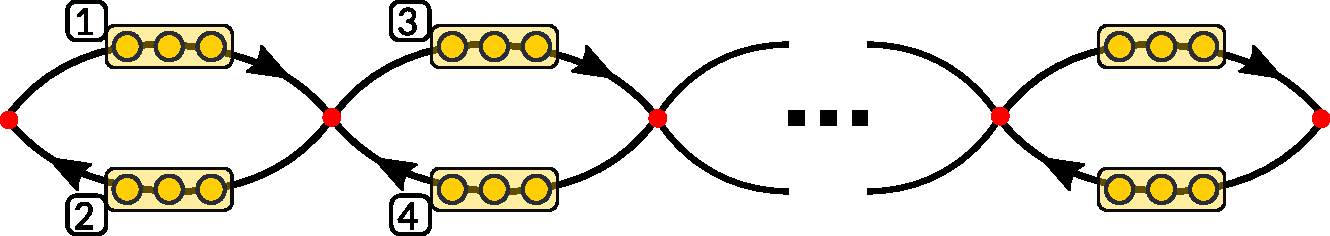
\includegraphics[width=\linewidth]{Figures/glasses.pdf}
    \vspace{0.05cm}
  %  \caption{Lattice}
    %\label{fig:gen_geom}
    \end{subfigure} %
    \hfill
    \begin{subfigure}{0.25\textwidth}
    \begin{equation*}
    \Qcircuit @C=0.2em @R=0.2em {
\lstick{m} & \gate{H} &       \ctrl{3} & \qw & \qw &\qw \\
\lstick{R} & \gate{H} &   \qw & \ctrl{3} & \qw & \qw \\
\lstick{R^{2}} & \gate{H} &  \qw & \qw & \ctrl{3} & \qw 
% \inputgrouph{1}{3}{2.2em}{\ket{h}}{2.5em}
\\
\lstick{\quad m} &  \qw &   \targ & \qw & \qw & \qw \\
\lstick{R} & \qw&   \qw &  \targ & \qw & \qw \\
\lstick{R^{2}} & \qw & \qw&   \qw &  \targ & \qw 
% \inputgrouph{4}{6}{2.2em}{\ket{g}}{2.5em}
}
\end{equation*}\vfill
    %\caption{Circuit}
  %  \label{figGS_prep}
\end{subfigure}
    \caption{Quasi one-dimensional lattice allowing for shallow ground state preparation of the quantum double model $D(D_4)$. Left: Yellow bars denote individual spins associated to edges, which are composed of three qubits each. Edge orientations are needed to define the vertex- and plaquette operators of the corresponding Hamiltonian and are drawn for the sake of concreteness. Right: Circuit for groundstate preparation per loop.}
    \label{fig:latticeGS}
\end{figure*}

%The ground state on this geometry, \caro{
%%I thought we always thought of this thing as being embedded in a sphere
%given an open boundary}, \caro{
%%it is entangled pairwise, it is not entangled along the chain
%is not entangled} and hence can be prepared in constant-depth.

The ground state on this geometry can be prepared in constant-depth. The ground state on an $n$-segment ladder is given by
\begin{equation}
    \ket{GS} = \sum_{g_1,g_2,\ldots,g_n} \ket{g_1,g_1,g_2,g_2,\ldots,g_n,g_n} \;.
\end{equation}
This state has no long-range entanglement and factorises into a sequence of Bell-pairs. 
However, entanglement is built up once one starts proliferating anyons via ribbon operators.
In fact, this geometry is sufficient to correctly represent the braiding statistics of the anyons. This holds as long as the ribbon paths used only \emph{touch}, but do not intersect.

The shallow circuit preparing this state is shown in Figure \ref{fig:latticeGS}.

We also examine fusion on a small two-dimensional graph, as shown in Figure \ref{fig:basketball}.

\begin{figure}
    \centering
    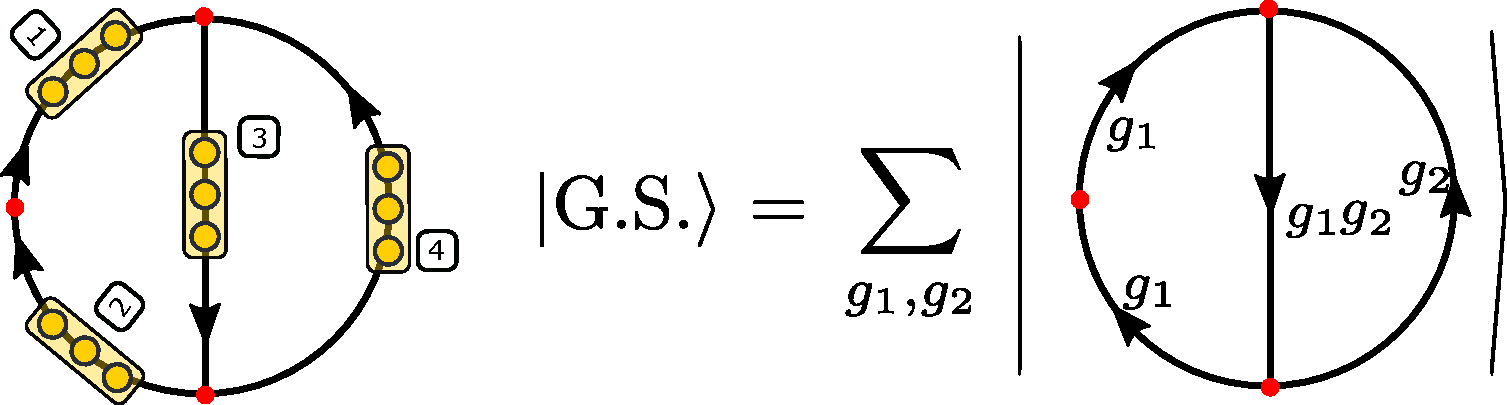
\includegraphics[width=\linewidth]{Figures/basketball.pdf}
    \caption{A small two-dimensional graph. Left: Yellow bars denote individual spins associated to edges, which are composed of three qubits each. Edge orientations are needed to define the vertex- and plaquette operators of the corresponding Hamiltonian and are drawn for the sake of concreteness. Right: The ground state on this small two-dimensional graph.}
    \label{fig:basketball}
\end{figure}




\subsection{Elemental protocols}
\textbf{Anyon fusion}
is the first and most basic protocol that can demonstrate Non-abelianness. 

After preparing the ground state, we apply two ribbon operators. One between sites $s_1$ and $s_2$, and the other between sites $s_2$ and $s_3$.
This creates two pairs of anyons and fuses them on site $s_2$. We then perform a partial charge measurement and flux readout for this site.
This experiment can be performed on both the braiding ladder and the two-dimensional small graph.

We can do this experiment for any anyon type. Here, we will give an example for the case of fusing the pure flux, $\Psi_m$ with itself. In contrast to the abelian case, this fusion is not restricted to yield vacuum. Instead we have
$$\Psi_m \times \Psi_m = 0 + \tilde{0} + \Sigma_m + \tilde{\Sigma}_m,$$ where $0$ is the vacuum, $\tilde{0}$ is the abelian flux corresponding to the other element of the centre of $D_4$, $r^2$ and the other two anyons are pure charge associated with the $\alpha_m$ representation of $D_4$ and the dyon of this pure charge and the abelian flux.

All four of these outcomes can be differentiated by reading out the flux and performing the partial charge measurement using $H_r$ or $H_{mr}$. For concreteness, we choose $H_r$. A discussion of this protocol implemented on a realistic hard-ware device and the numerical simulation of the latter are shown in Section \ref{sec:num:fusion}.


%The $H_m$-reduced charge measurement doesn't see the difference between $0$ and $\Psi_m$.

%The results of numerical for these two experiments are shown in Figure \ref{fig:fusion_glass} and \ref{fig:fusion_basketball}.
%
%Here we see the four peaks corresponding to the four fusion outcomes for both geometries.
%For further discussion of the numerical results, see Section \ref{sec:num}.

\textbf{Anyon Braiding.} The second phenomenon that gives the non-abelian anyons their name is the fact that the image of the braid group, as represented by physically braiding these anyons, is non-abelian. 
This means that the order of interchanges matter, i.e. $\sigma_{12}\sigma_{23} \neq \sigma_{23}\sigma_{12}$, where $\sigma_{ii+1}$ are clockwise interchange of particle $i$ and $i+1$, the generators of the braid group.


\begin{figure}
    \centering
    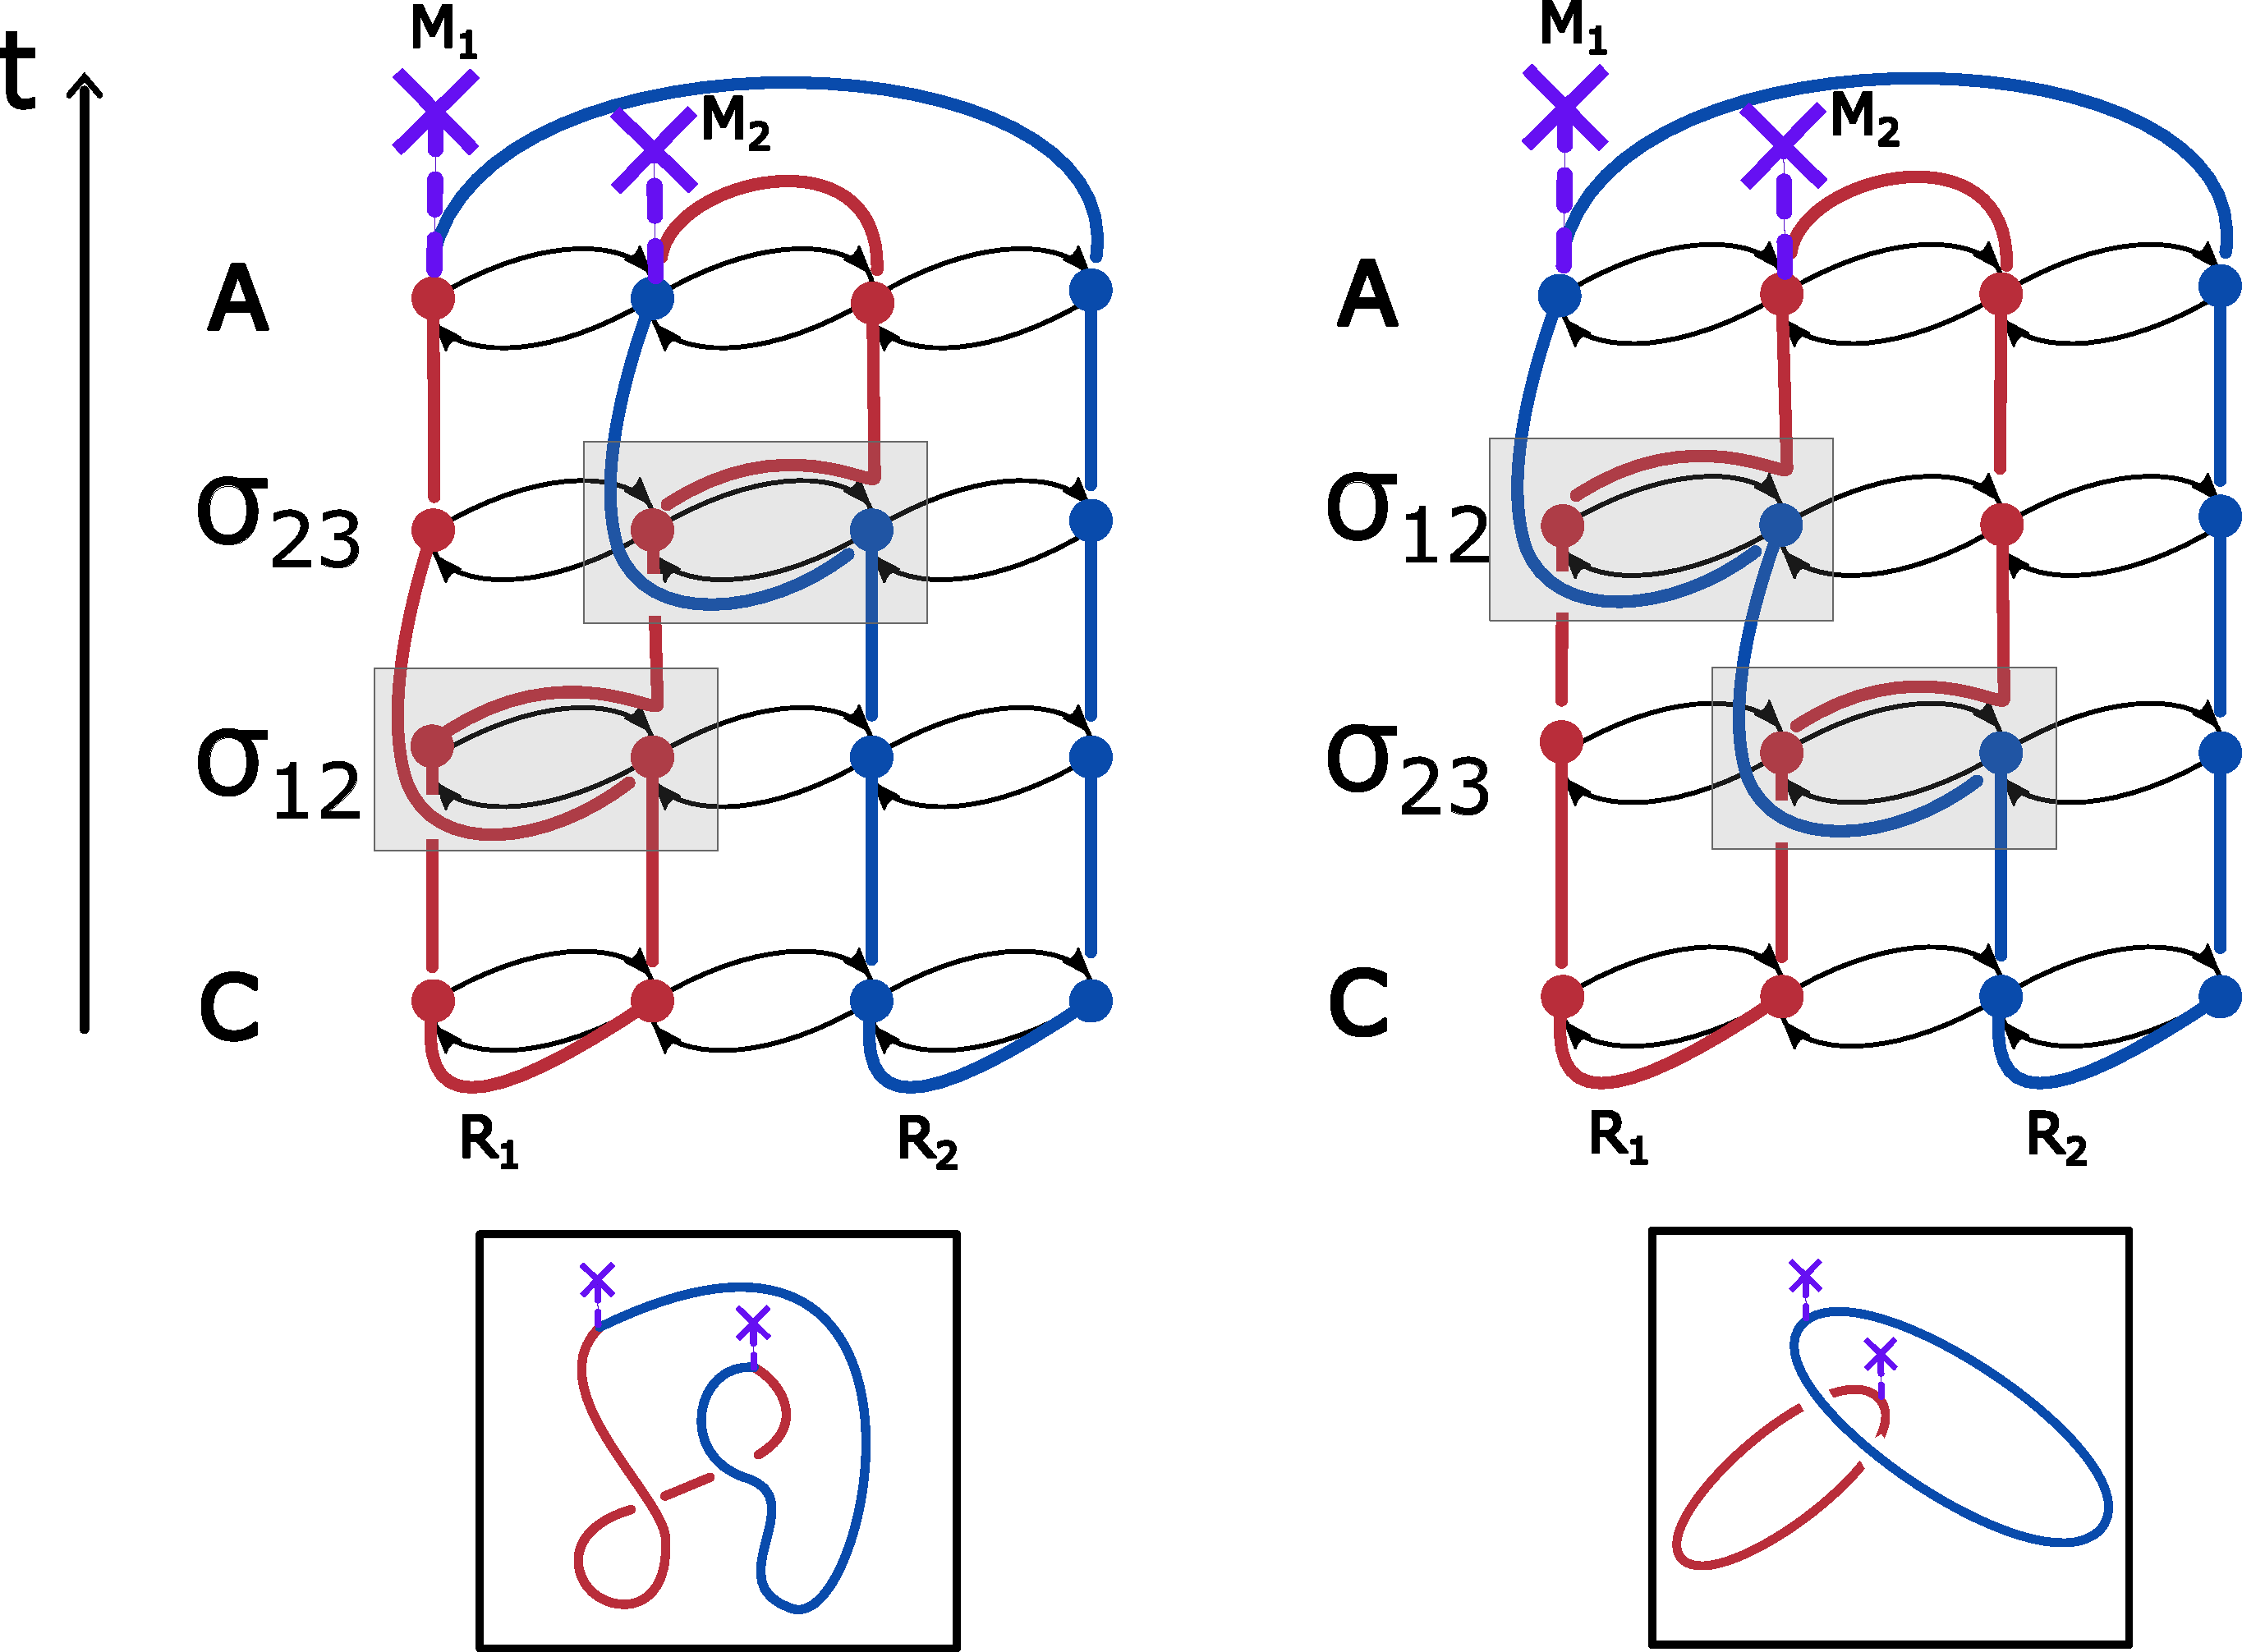
\includegraphics[width=\linewidth]{Figures/fluxBRAID.pdf}
    \caption{The two braiding protocols, differing only in order of exchange of two anyons. Protocol a) will have 4 fusion outcomes, while protocol b) can only produce vacuum.}
    \label{fig:flux_braid}
\end{figure}

The braiding procedures we want to implement to show this fact are shown in Figure \ref{fig:flux_braid}. We create two pairs of anyons from the vacuum, perform two interchanges $\sigma_{12}, \sigma_{23}$, and then fuse pairwise. Then we repeat the same protocol with the inverted order of the interchanges, i.e., $\sigma_{23} \sigma_{12}$. For concreteness, we again consider pairs for pure fluxes $\Psi_m$. 
\caro{Change figure such that first is trivial and second is non-trivial.}


In the first version, we annihilate the pairs that have a fixed fusion channel. Given that they are created from the vacuum they will fuse to the vacuum.
In the second version, we annihilate the pairs whose fusion channel is not fixed, hence all four fusion outcomes are expected. We see that the two braidings indeed produce two different states. 

For further discussion of a concrete implementation and numerical results, see Section \ref{sec:num}.

\subsection{Anyon interferometry}\label{subsec:Intef}



%In order to access full data of the S- and T-matrix, amplitude and phase of its elements, we must devise an interference protocol.

In order to measure the relative phase between different braiding processes, we need to devise an interference protocol. This is done by setting up a control qubit $c$, whose states are entangled with different braiding protocols
\begin{equation}
    \ket{\psi}_c\ket{\text{GS}} \rightarrow \ket{0}_c \ket{\Psi_0} + \ket{1}_c \ket{\Psi_1},
\end{equation}
where $\Psi_i$ are the two wave functions of the matter degrees of freedom corresponding after two different braiding operations.

If the charge content of the two states is the same they may only differ by a constant. Hence we can write
\begin{equation}
    \ket{0}_c \ket{\Psi_0} + \ket{1}_c \ket{\Psi_1} = (\ket{0}_c + C_{01}\ket{1}_c)\ket{\Psi_0},
\end{equation}
and by the means of tomography on the control qubit $c$ we can extract the relative constant $C_{01}$.

For a suitable choice of two braiding protocols, this constant reveals the elements of S- and T-matrix, see Figure \ref{fig:intef_example}.

\textbf{S-matrix elements.}
To measure the S-matrix elements, we create a superposition of two states by conditioning an equal time (closed) ribbon operator shown in blue in Fig.~\ref{fig:S-mat} on the control qubit . 





Note that the S-matrix appearing in Figure is normalized:
\begin{equation}
    \tilde{S}(a,b) = \frac{|D_4|}{d_a d_b}S(a,b),
\end{equation}
which makes $|\tilde{S}(a,b)| \leq 1$.



The straight forward way to do this, is to condition the entire ribbon operator (see Figure \ref{fig:cond_ex}).  In conjunction with the calibration shown in Figure \ref{fig:phase_check}, this is conceptually the same as the ideal protocol in Figure \ref{fig:intef_example}. 
The calibration is done to make sure there is no dynamical phase accumulated by applying the $b$ ribbon itself.
However, in this protocol every single qubit gate of the ribbon operator becomes a two qubit gate and every two qubit gate becomes a three qubit gate (unitarily similar to a Toffoli gate). Hence, the number of entangling gates grows fast.

A smarter alternative is to condition the anyon type of the ribbon (see Figure \ref{fig:cond_flav}). In this case we identify where the ribbon operators for the two anyon types differ, and condition only those operations. The circuit for this can be much shorter, see Fig. \ref{fig:cond_flav} for an example. In particular, for the case of $D(D_4)$, it turns out, that it is easier to compare the linking of anyons $a$ and $b$ to the linking of $a$ and $0 \oplus \tilde 0$, then comparing it to the linking of $a$ with vacuum. Thus, we condition whether we apply the ribbon $b$ or the ribbon corresponding to $0 \oplus \tilde 0$. 

However, this protocol requires additional knowledge of the theory. Concretely, if we are interested in the S-matrix element $S_{ab}$, we need the additional knowledge of  $S(a, 0)$ and $S(a, \tilde{0})$. Both can in fact be measured directly with a simple protocol since $0$ and $\tilde{0}$ are abelian, see Appendix \ref{app:abl}.
Since $S(a, 0) = S(a, \tilde{0}) = 1$, we can just read off $S(a,b)$ after tomographing the control qubit.

In our example, we will fix $b$ to be pure flux $\Psi_m$ again due to the relative simplicity of its ribbon operators. For the other anyon we will choose one of the following $a\in\{\Psi_m,\tilde{\Psi}_m, \Phi_r \}$ which gives us all three possible values of the S-matrix elements for the $D_4$ theory, $\{1, -1, 0\}$.



The exact method of tomography will be presented alongside the numerical result in Section \ref{sec:num}. 



The result is illustrated in Fig.~\ref{fig:flavCond}.

%In that example, the control qubit is selecting between two different ribbon operators. The first one is the ribbon creating the pure flux $\Psi_m$ and the other one corresponds to the reducible two-dimensional representation $0 \oplus \tilde{0}$.


% One can also look at the case where we condition the existence of the ribbon as selecting between two types, $\Psi_m$ and the vacuum (represented as $0 \oplus 0$), see Figure \ref{fig:flavCond} (left).

% We will use both schemes in our phase-sensitive S-matrix experiment.

%First, depending on the state of the control qubit, $c$ the ribbon is either for an irrep label $b$ of $D(D_4)$, corresponding to an anyon, or for the reducible representation\footnote{The ribbon operator application scheme is the same for ribbons labelled by reducible and irreducible representations.} $0\oplus\tilde{0}$ spanned by vectors $\{\ket{e;1}, \ket{r^2;1}\}$.


%Second, depending on the state of the control qubit $c$, the ribbon is either for the irrep $b$ or for the reducible representation $0\oplus 0$. This basically means that if the state of the control is $\ket{0}_c$ then we do nothing.

%
%However, given that every operation of the conditioned ribbon is conditioned on $c$, the complexity of the circuit for the second option is larger than for the first option where only some operations are conditioned on $c$.




\begin{figure}
\begin{equation*}
\Qcircuit @C=0.5em @R=0.7em @!R{
\lstick{c} & \ctrl{3} & \qw& \ctrl{1}& \qw\\
\lstick{m} & \qw & \qw & \targ& \qw\\
\lstick{R} & \qw  & \qw & \qw& \qw\\
\lstick{R^{2}} & \targ  & \qw & \qw& \qw\\
\lstick{\text{aux}} &  \ctrl{-1} & \qw& \qw& \qw
}%
\qquad \qquad \qquad
\Qcircuit @C=0.5em @R=0.7em @!R{
\lstick{c} & \ctrl{1} & \qw\\
\lstick{m} & \targ & \qw \\
\lstick{R} & \qw  & \qw \\
\lstick{R^{2}} & \targ  & \qw \\
\lstick{\text{aux}} &  \ctrl{-1} & \qw
}
%
%\Qcircuit @C=0.5em @R=0.7em @!R{
%\lstick{c} & \ctrl{2} & \qw\\
%\lstick{m} & \qw & \qw \\
%\lstick{R} & \ctrl{2}  & \qw \\
%\lstick{R^{2}} & \qw  & \qw \\
%\lstick{\text{aux}} &  \targ & \qw
%}
\end{equation*}
\caption{Controlled multiply circuits of an elementary triangle of a ribbon operator conditioned on a control qubit $c$. Left. Implementing $\Psi_m$ vs vacuum, represented as $0\oplus 0$. Right. Implementing $\Psi_m$ vs $0\oplus\tilde{0}$.}
%Left:  
%
%
%used when anyon moves along a edge $i$ encoded by the middle three bits, control bit $c$ selects between pure flux $\Psi_m$ and reducible label . 
%
%
%Center: controlled multiply circuit used when anyon moves along a edge $i$ encoded by the middle three bits, control bit $c$ selects between pure flux $\Psi_m$ and reducible label $0\oplus 0$, i.e. doing nothing. 
%
%
%Right: controlled conjugation circuit used when anyon crosses along a edge $i$ encoded by the middle three bits, control bit $c$ selects between pure flux $\Psi_m$ and reducible label $0\oplus\tilde{0}$ or $0\oplus 0$. Note: ribbons can also be associated with reducible representations of $D(G)$ as long as they are closed, if we require a well-defined topological charge of the end state, the scheme for applying ribbon operators associated with the reducible representations is the same as for the irreducible representations.}
\label{fig:flavCond}
\end{figure}





\begin{figure*}
\centering

\begin{subfigure}{0.47\textwidth}
    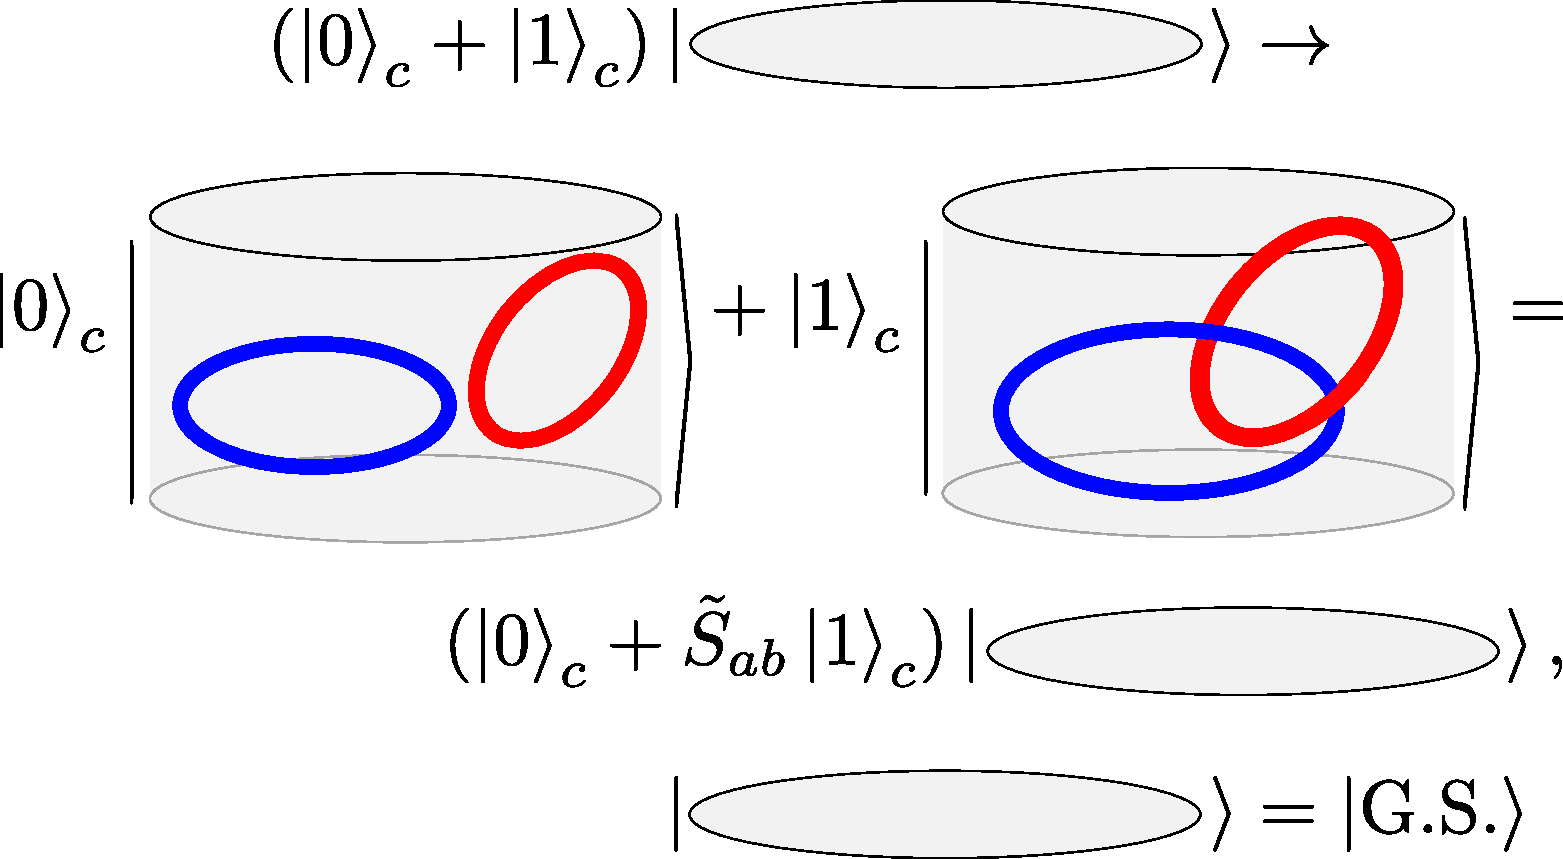
\includegraphics[width = \linewidth]{Figures/intef_example.pdf}
    \caption{The ideal interferometry scheme for measuring the S-matrix elements. The two possible braiding are appropriately entangled with the controlling bit $c$, which is achieved by controlled ribbon operators.}
    \label{fig:intef_example}
\end{subfigure}\hfill
\begin{subfigure}{0.47\textwidth}
    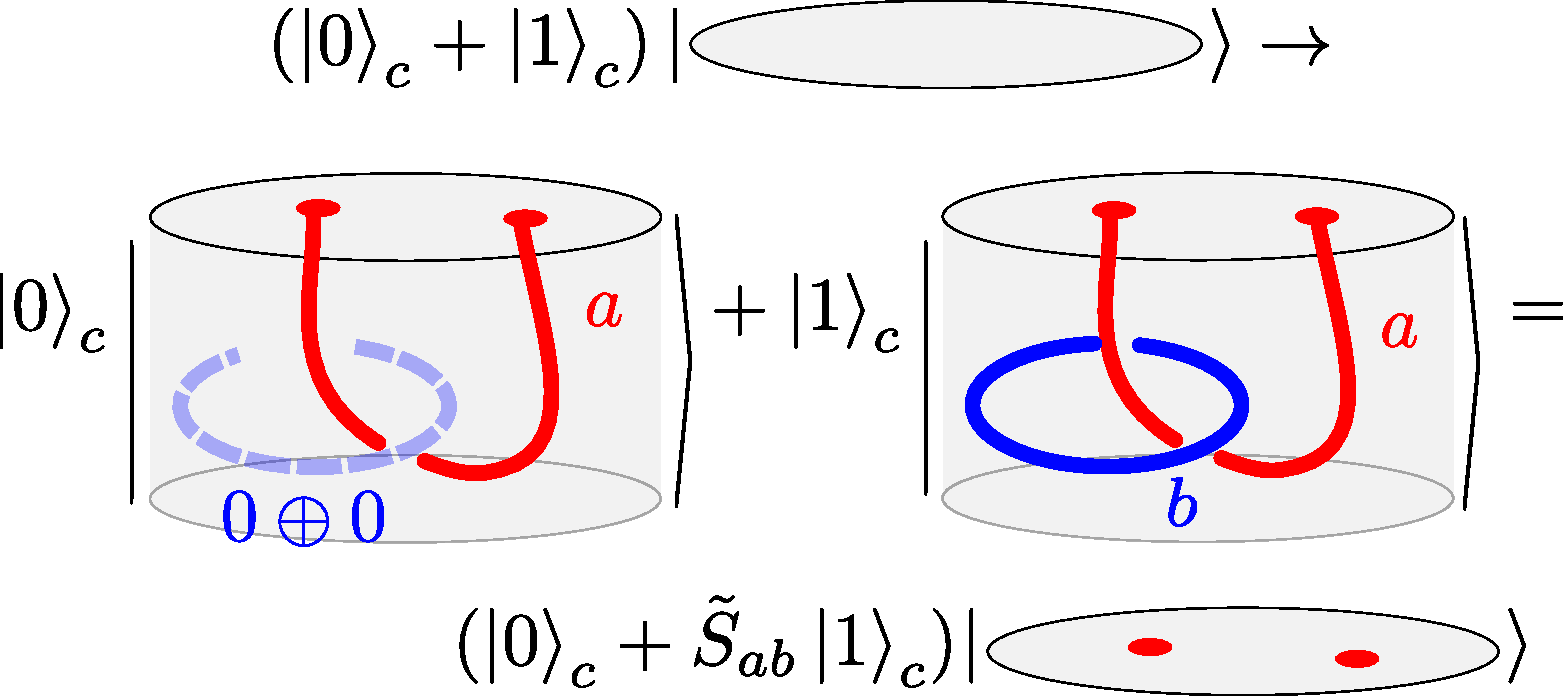
\includegraphics[width=\linewidth]{Figures/intefEx.pdf}
    \caption{Conditioning the existence of the ribbon. The ribbon $\Psi_m$ is only applied, if the state of the control qubit is $\ket{1}_c$. Equivalently, conditioning whether to apply $\Psi_m$ or the reducible representation $0\oplus 0$. \jovan{Fix the caption.}}
    \label{fig:cond_ex}
\end{subfigure}
%\begin{subfigure}{0.47\textwidth}
%    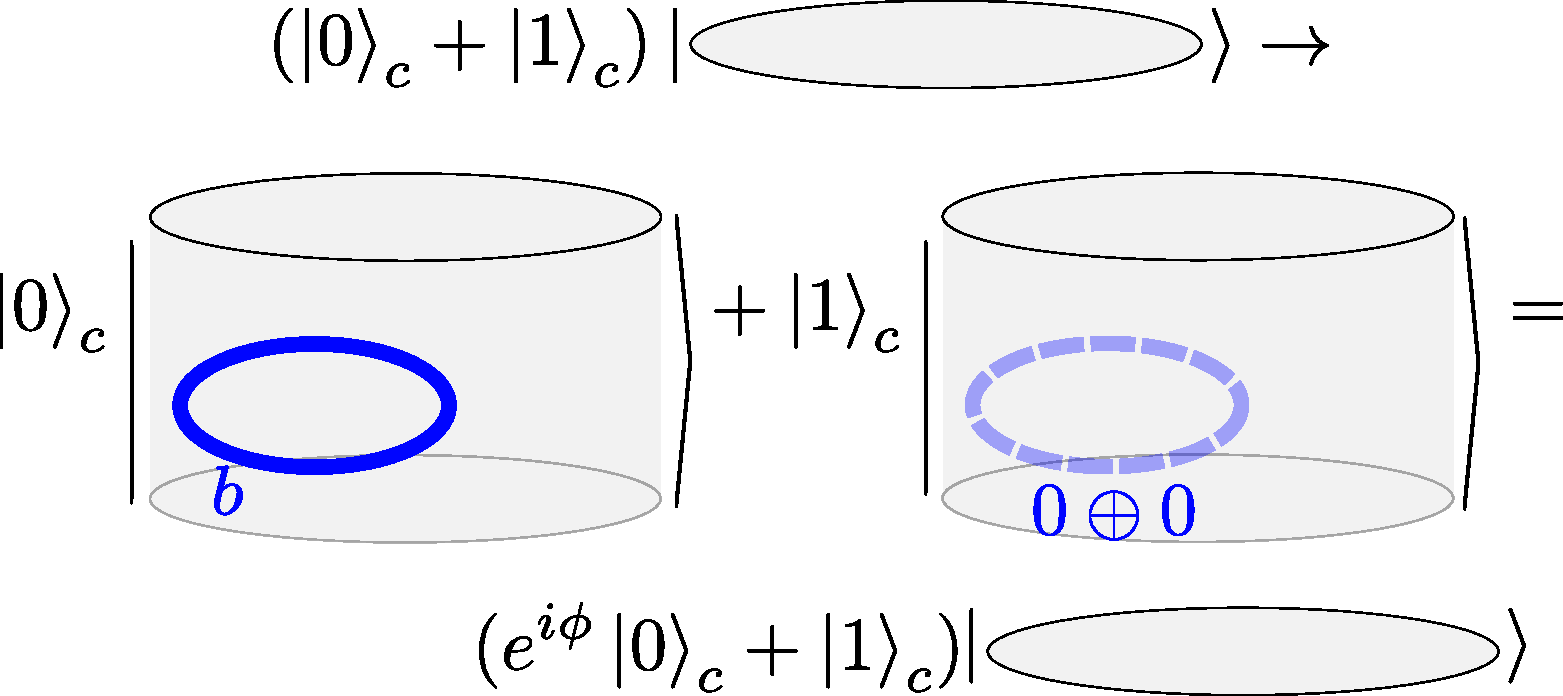
\includegraphics[width=\linewidth]{Figures/phaseCheck.pdf}
%    \caption{Phase check. Making sure to remove any phase that is due to the application of the closed ribbon $\Psi_m$ itself.}
%    \label{fig:phase_check}
%\end{subfigure} MOVE TO THE SOME APPS

\vspace{15pt}

\begin{subfigure}{0.47\textwidth}
    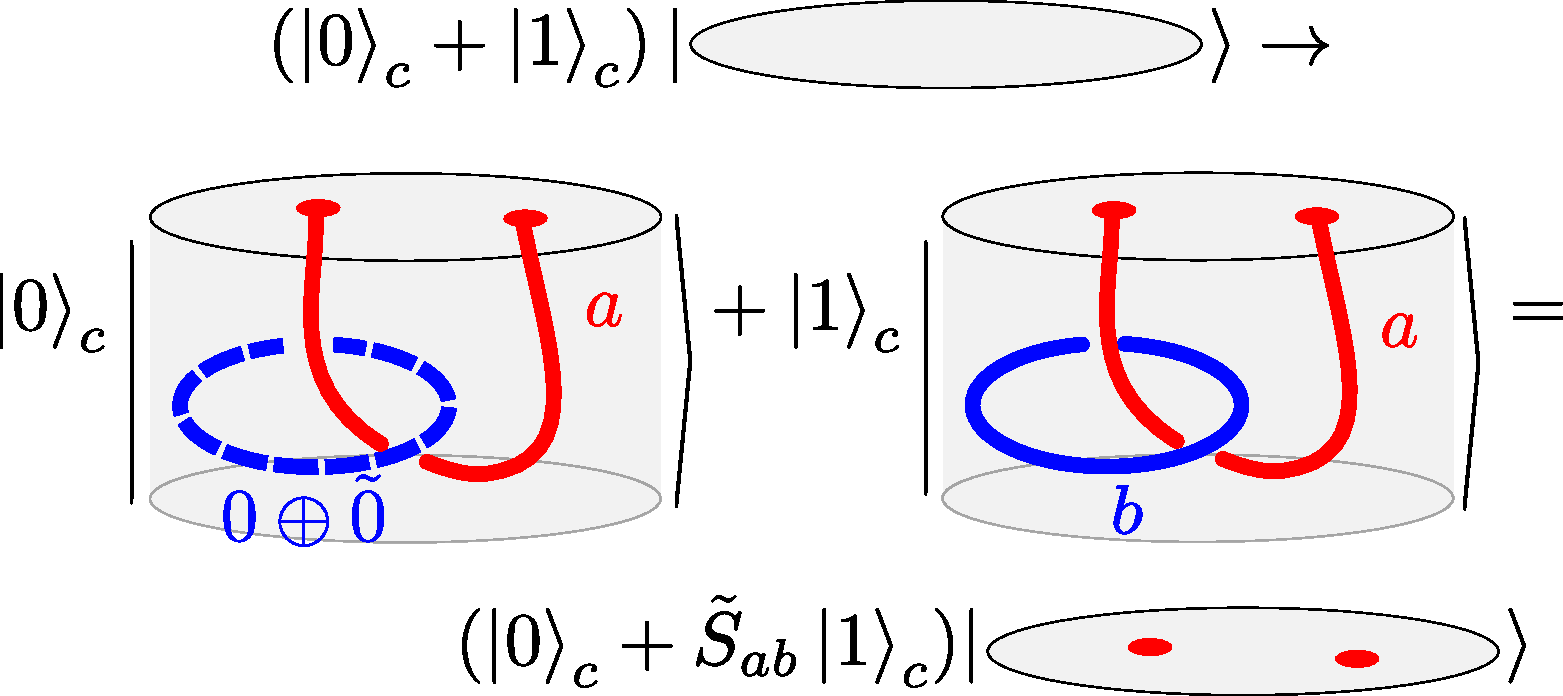
\includegraphics[width=\linewidth]{Figures/intefFlav.pdf}
    \caption{Conditioning the flavour of the ribbon, if the state of the control bit is $\ket{0}_c$ then the flavour is the reducible representation $0\oplus\tilde{0}$ and $\Psi_m$ otherwise. This is the shallowest protocol in terms of total compiled circuit depth.}
    \label{fig:cond_flav}
\end{subfigure}

\caption{The interference protocols used for phase sensitive measurement of the (normalized) S-matrix elements  $\tilde{S}(a,b) = \frac{|D_4|}{d_a d_b}S(a,b)$\caro{general b? adjust figures?, for
$S(a, \Psi_m)$ for $a\in\{\Psi_m, \tilde{\Psi}_m, \Psi_r\}$.}}
\label{fig:S-mat}
\end{figure*}

\begin{figure*}
\centering
\begin{subfigure}{0.47\textwidth}
    \centering
    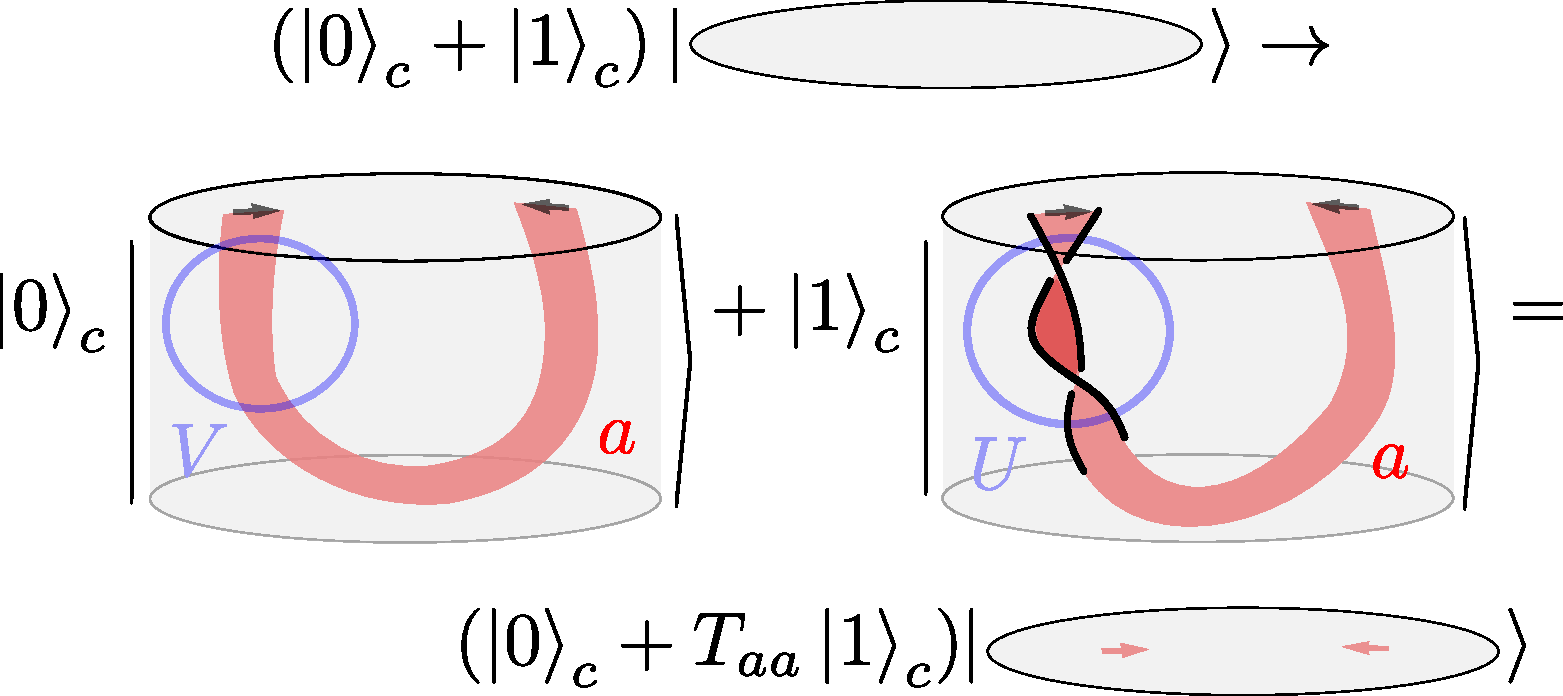
\includegraphics[width = \linewidth]{Figures/Tmat2.pdf}
    \caption{Interference protocol for measuring the phase of the T-matrix elements. Note: $|T_{aa}| = 1$ for all anyons $a$. The inference is done between two paths that differ by only one twist. We have restored the two-dimensionality of the ribbons in our representation in order to showcase the extra twist.}
    \label{fig:Tmat}
\end{subfigure}\hfill
\begin{subfigure}{0.47\textwidth}
\begin{equation*}
\Qcircuit @C=0.5em @R=0.7em @!R{
\lstick{c}&\qw&\ctrl{1}&\qw& \gate{X}&\qw&\ctrl{1}&\qw&\gate{X}&\qw\\
\lstick{\text{aux}}&\qw&\multigate{1}{U}&\qw &\qw&\qw&\multigate{1}{V}&\qw&\qw&\qw\\
\lstick{GF}&\qw&\ghost{U}&\qw&\qw&\qw&\ghost{V}&\qw&\qw&\qw
}
\end{equation*}
\caption{A circuit that depending on the state of the control bit $c$ either applies a unitary $U$ or $V$ onto the joint gauge field ($GF$) and auxiliary (aux) degrees of freedom.}
\label{fig:condcirq}
\end{subfigure}
\caption{The interferometry scheme to measure the phase difference between two paths alongside with a circuit diagram implementing the difference of the two paths.}
\label{fig:tmatfull}
\end{figure*}



\textbf{T-matrix elements}

In this section, we will describe the interference protocol for measuring the matrix elements of the diagonal T-matrix, or the spin of the anyons.
Here we note that ribbon operators are in-fact ribbons in space-time, hence they can acquire a twist.
Each twist contributes a phase factor to the wavefunction, $T_{aa} = e^{i\theta_a}$. 

The protocol is illustrated in Figure \ref{fig:Tmat}. We identify where the twisted and untwisted paths of a ribbon operator associated with some anyon $a$ differ and apply a controlled circuit of the form illustrated in Figure \ref{fig:condcirq} accordingly. If for the untwisted (twisted) version, we need to apply the unitary $U$ ($V$), the circuit implementing is straight-forward and shown in Figure \ref{fig:condcirq}.

The endpoint of the two ribbons are on the same site, hence the charge content is the same and we can factor out the gauge field wavefunction. 
The control qubit is in a pure state (assuming there is no noise) that we can tomograph and read off the twisting phase.


\section{Numerical Experiments}\label{sec:num}

In this section, we provide numerical evidence for the feasibility of our proposal on state of the art NISQ devices. We performed simulations using Google's 'cirq\_google' python package on Google's cloud computing platform 'Google Colab'. This package executes the quantum trajectory simulation of the circuit using the Kraus operators obtained from the direct Pauli transfer matrix tomography on various single and two qubit gates on the Sycamore chip \cite{weber}. This chip comes with two principle constraints. First, we can only perform two-qubit gates between adjacent qubits. Second, there is a limited set of gates that can be implemented. 


Knowing the characteristics of the single and two-qubit gates, and single- and multi-qubit readout performances of the chip \cite{weber} we have chosen a suitable part of the chip for our simulations. A similar setup would be suitable for an actual experiment on the Sycamore chip. However, the optimal allocation of recourses will be chip depended. The layout we used is shown in Figure \ref{fig:fusion_setup}.

Given that we argue for feasibility of these experiments, we need to ask how well this numerical scheme, will reproduce the actual measurements.
\caro{which heuristics?} Heuristics shows that it is in fact a good approximation of what we expect to see from the actual experiment \cite{}, even if it neglects any cross-talk between qubits that are not directly coupled by the circuit.

The number of qubits we could simulate classically using this software is limited to 30 qubits, which is less than the number of qubits currently available on an actual machine. To see how this comes about, let us note that even though in our protocols there are only a few non-Clifford gates, we can not exploit the advantage of Clifford simulators because we simulate \emph{noisy circuits}. 
%A Clifford gate maps a Pauli string into a Pauli string, which implies a simple Pauli transfer matrix, i.e., only one Krauss operator. Hence it cannot be noisy (non-unitary).
%If we are interested in Noisy simulations we are automatically outside Clifford group and we cannot get around doing a quantum circuit simulation in-full.}


\subsection{Elemental Protocols}

In this section, we present the simulation results for the fusion and braiding experiments.

\textbf{Circuit Characteristics.} However, before we present the results, we report on the qubit layout used for the fusion and braiding experiments, as well as circuits depths achieved, in order to put the noise observed in a useful context.

\emph{Fusion.} 
The exact ribbon operators and the layout of the qubits on the Sycamore chip used in the fusion experiment is shown in Fig.~\ref{fig:fusion_setup}.
\begin{figure}
	\centering
	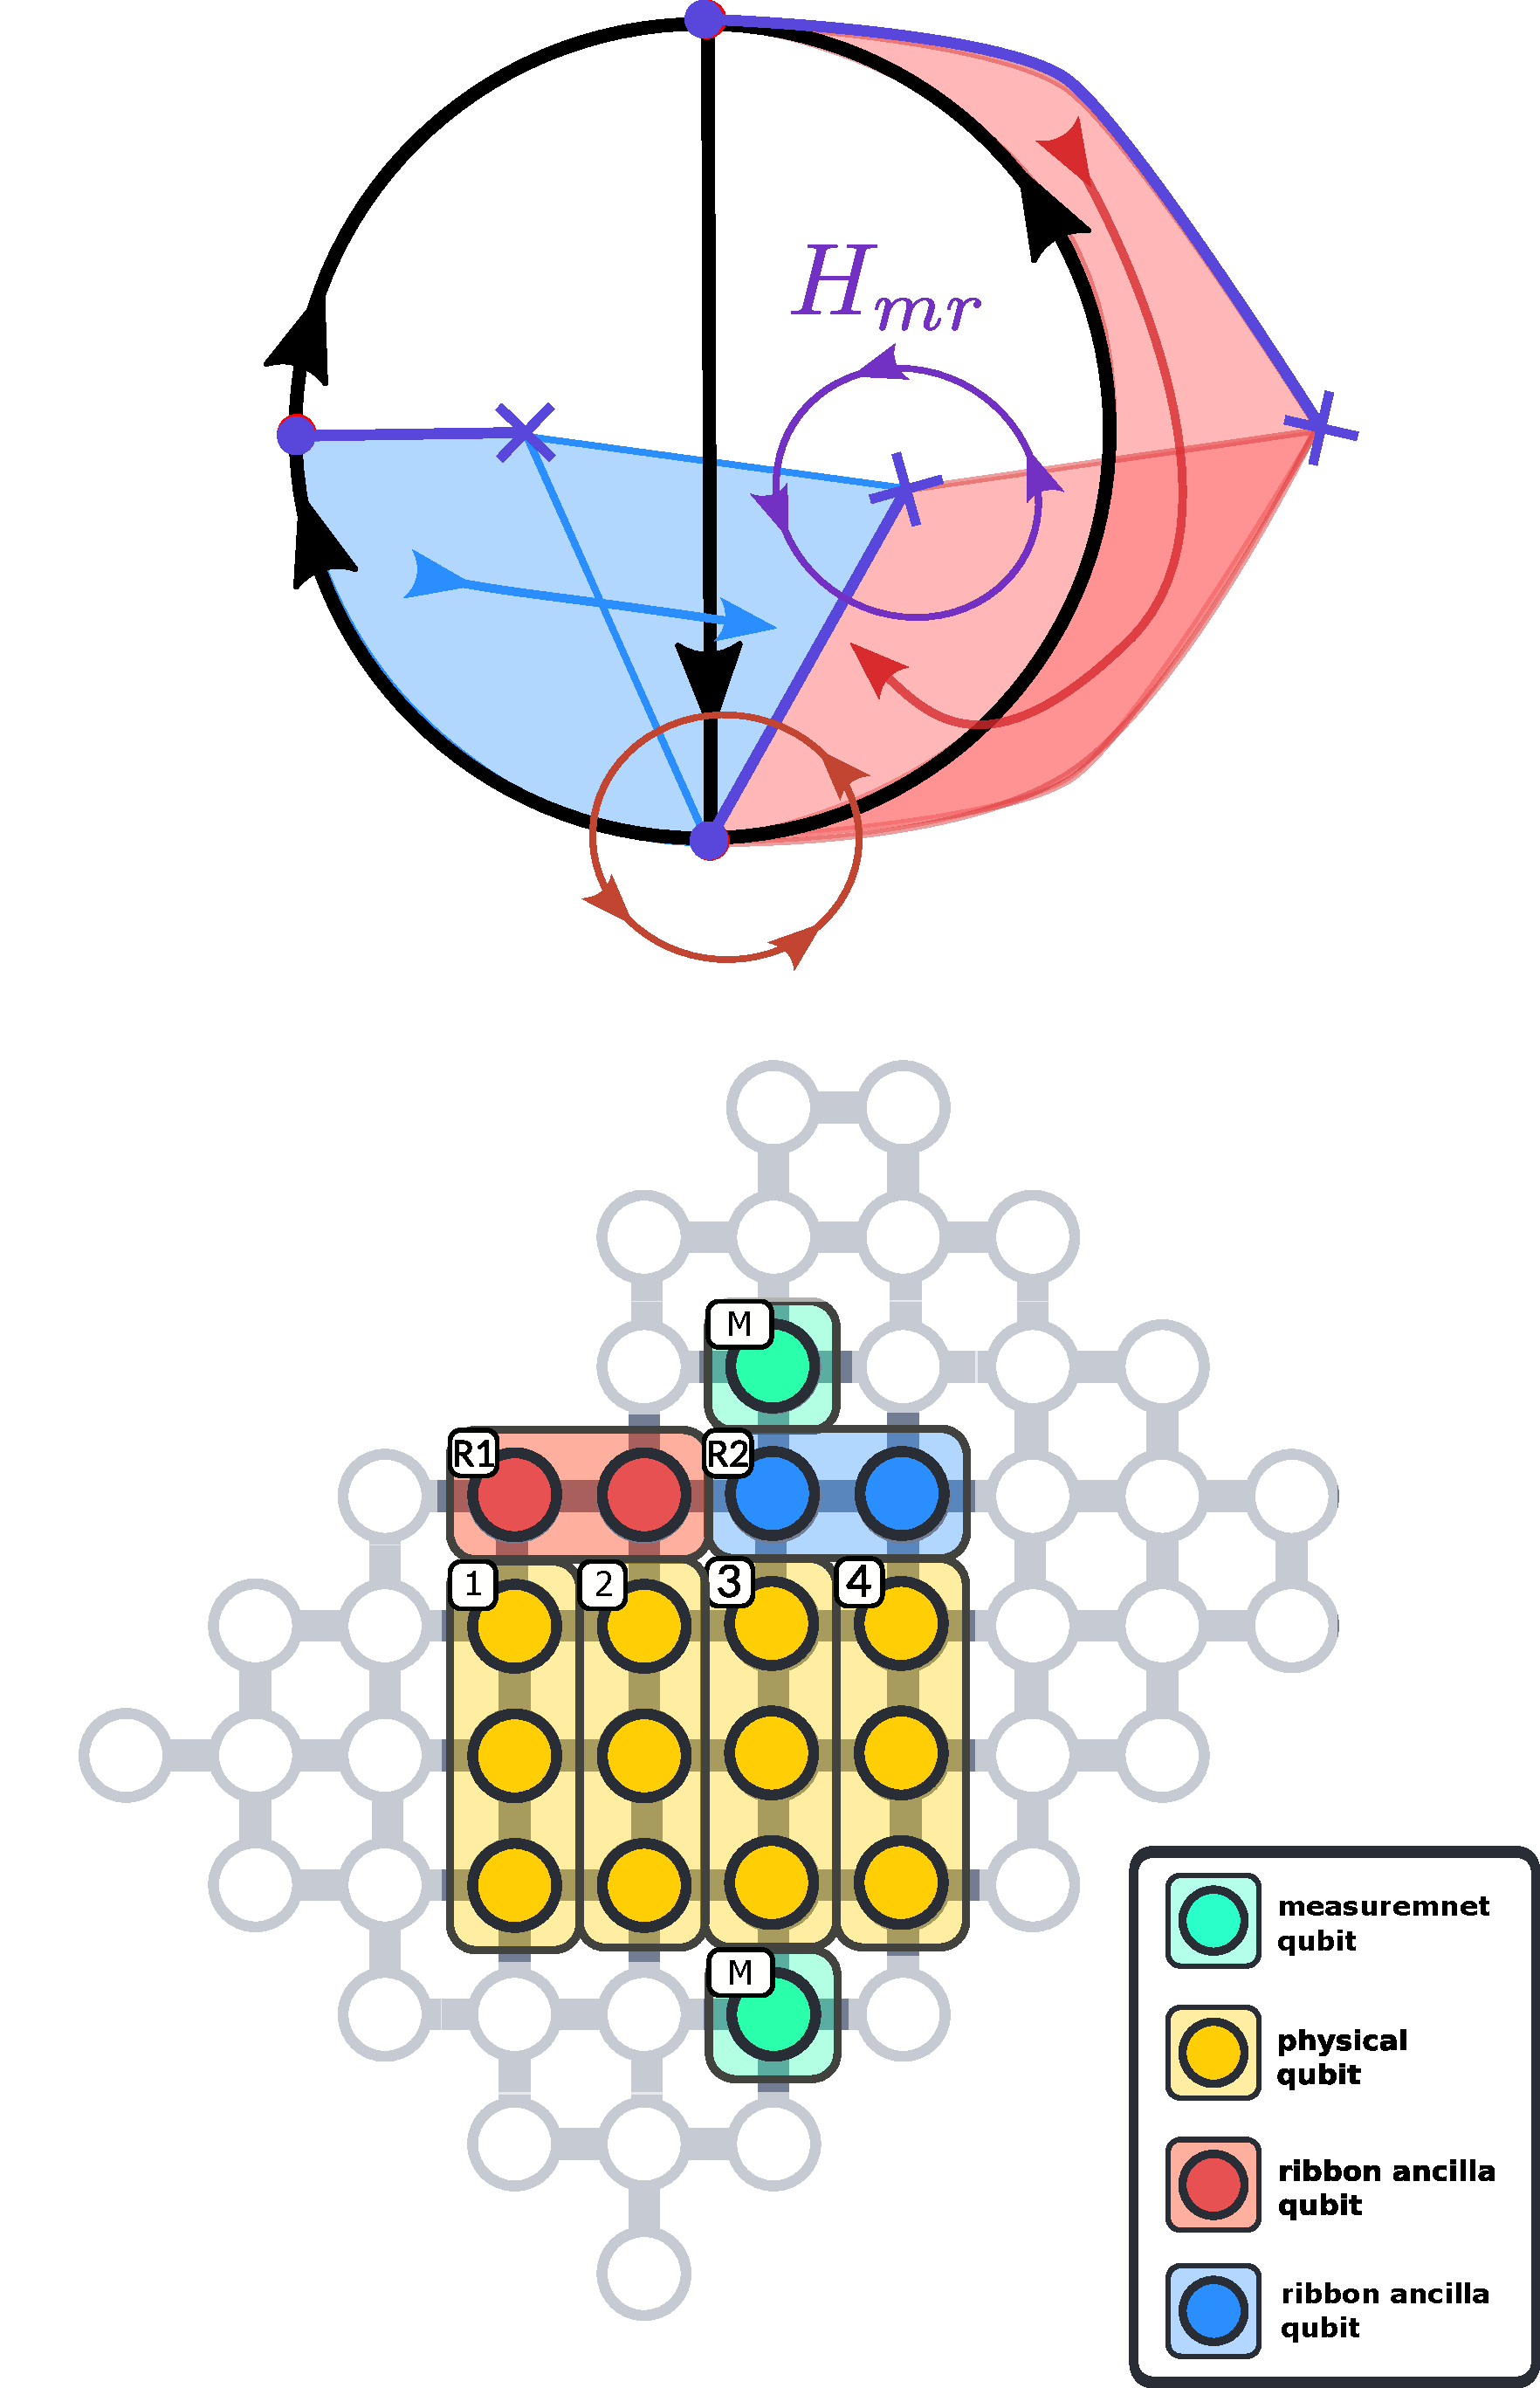
\includegraphics[width=\linewidth]{Figures/basket_fusion.pdf}
	\caption{(Top) The ribbon operators for the fusion of two $\Psi_m$ anyons on a small planar graph. The purple circle marks the plaquette on which we perform the $H_{mr}$-partial charge measurement. The red circle marks the vertex on which we measure the flux, together they form the site on which fusion occurs. (Bottom) The circuit layout on the Sycamore chip we used to simulate the fusion experiment.}
	\label{fig:fusion_setup}
\end{figure}

Using the circuits listed in Sec.~\ref{subsec:enc} to implement the ribbon operators defined in Sec.~\ref{sec:ribbon_ops} generates a circuit that is not directly implementable on the Sycamore chip due to the constraints mentioned above. We first need to implement swap gates such that all the multi-qubit gates appearing in the original circuit are acting on adjacent qubits. In addition, we need to compile multi-qubit gates into native single- and two-qubit coupler gates. In our case we chose the CZ gate as the coupler (two-qubit) gate. The single qubit gates are unrestriced.  

The additional swaps make up a considerable portion of all coupling gates used in the numerical experiments and hence the positioning of qubit is one of the key factors in minimising the circuit depth.

It is also worth noting that not all anyons are equal in complexity. The $r-$dyons ribbon require considerably deeper circuits since the group multiplication controlled by the elements of the $\mathcal{C}_r$ conjugacy class always involve at least one Toffoli gate. Let us recall that the Toffoli gate needs to be compiled into a depth-6 circuit using the CZ as the two qubit coupler, however this neglects any swaps needed to place the qubits acted on by the CZ gates adjacent to one another. Hence, reducing the number of Toffoli gates is the main heuristic approach when designing the experiments while keeping the depth minimal.

\caro{maybe move to next section: However, minimising the circuit depth at all costs is not always the best heuristic approach for circuit design. In the interference protocols discussed in the next section, it is paramount to reduce the number of gates acting on the control qubit even if it leads to deeper circuits.} 

For the fusion of $\Psi_m$-fluxes on the small planar graph, we obtained a device-ready circuit of depth 70. This circuit prepares the ground state, implements the ribbon operators and performs a partial charge measurement. 
%For the fusion of $\Psi_m$-fluxes on the small planar graph, we obtained a circuit of depth 17. This circuit prepares the ground state, implements the ribbon operators and perform a partial charge measurement. In this depth the auxiliary swaps are included. The circuit once compiled into one that only uses CZ reaches the depth of 70.
On the braiding ladder the same protocol leads to a much shorter circuit of depth 37. This is due to a significantly simpler ground state preparation.\caro{comment on layout and ribbons}

\emph{Braiding.} The ribbon operators for the two braiding protocols and the qubit layout on the Sycamore chip are shown in Fig.~\ref{fig:braiding_setup}.
\begin{figure}
	\centering
	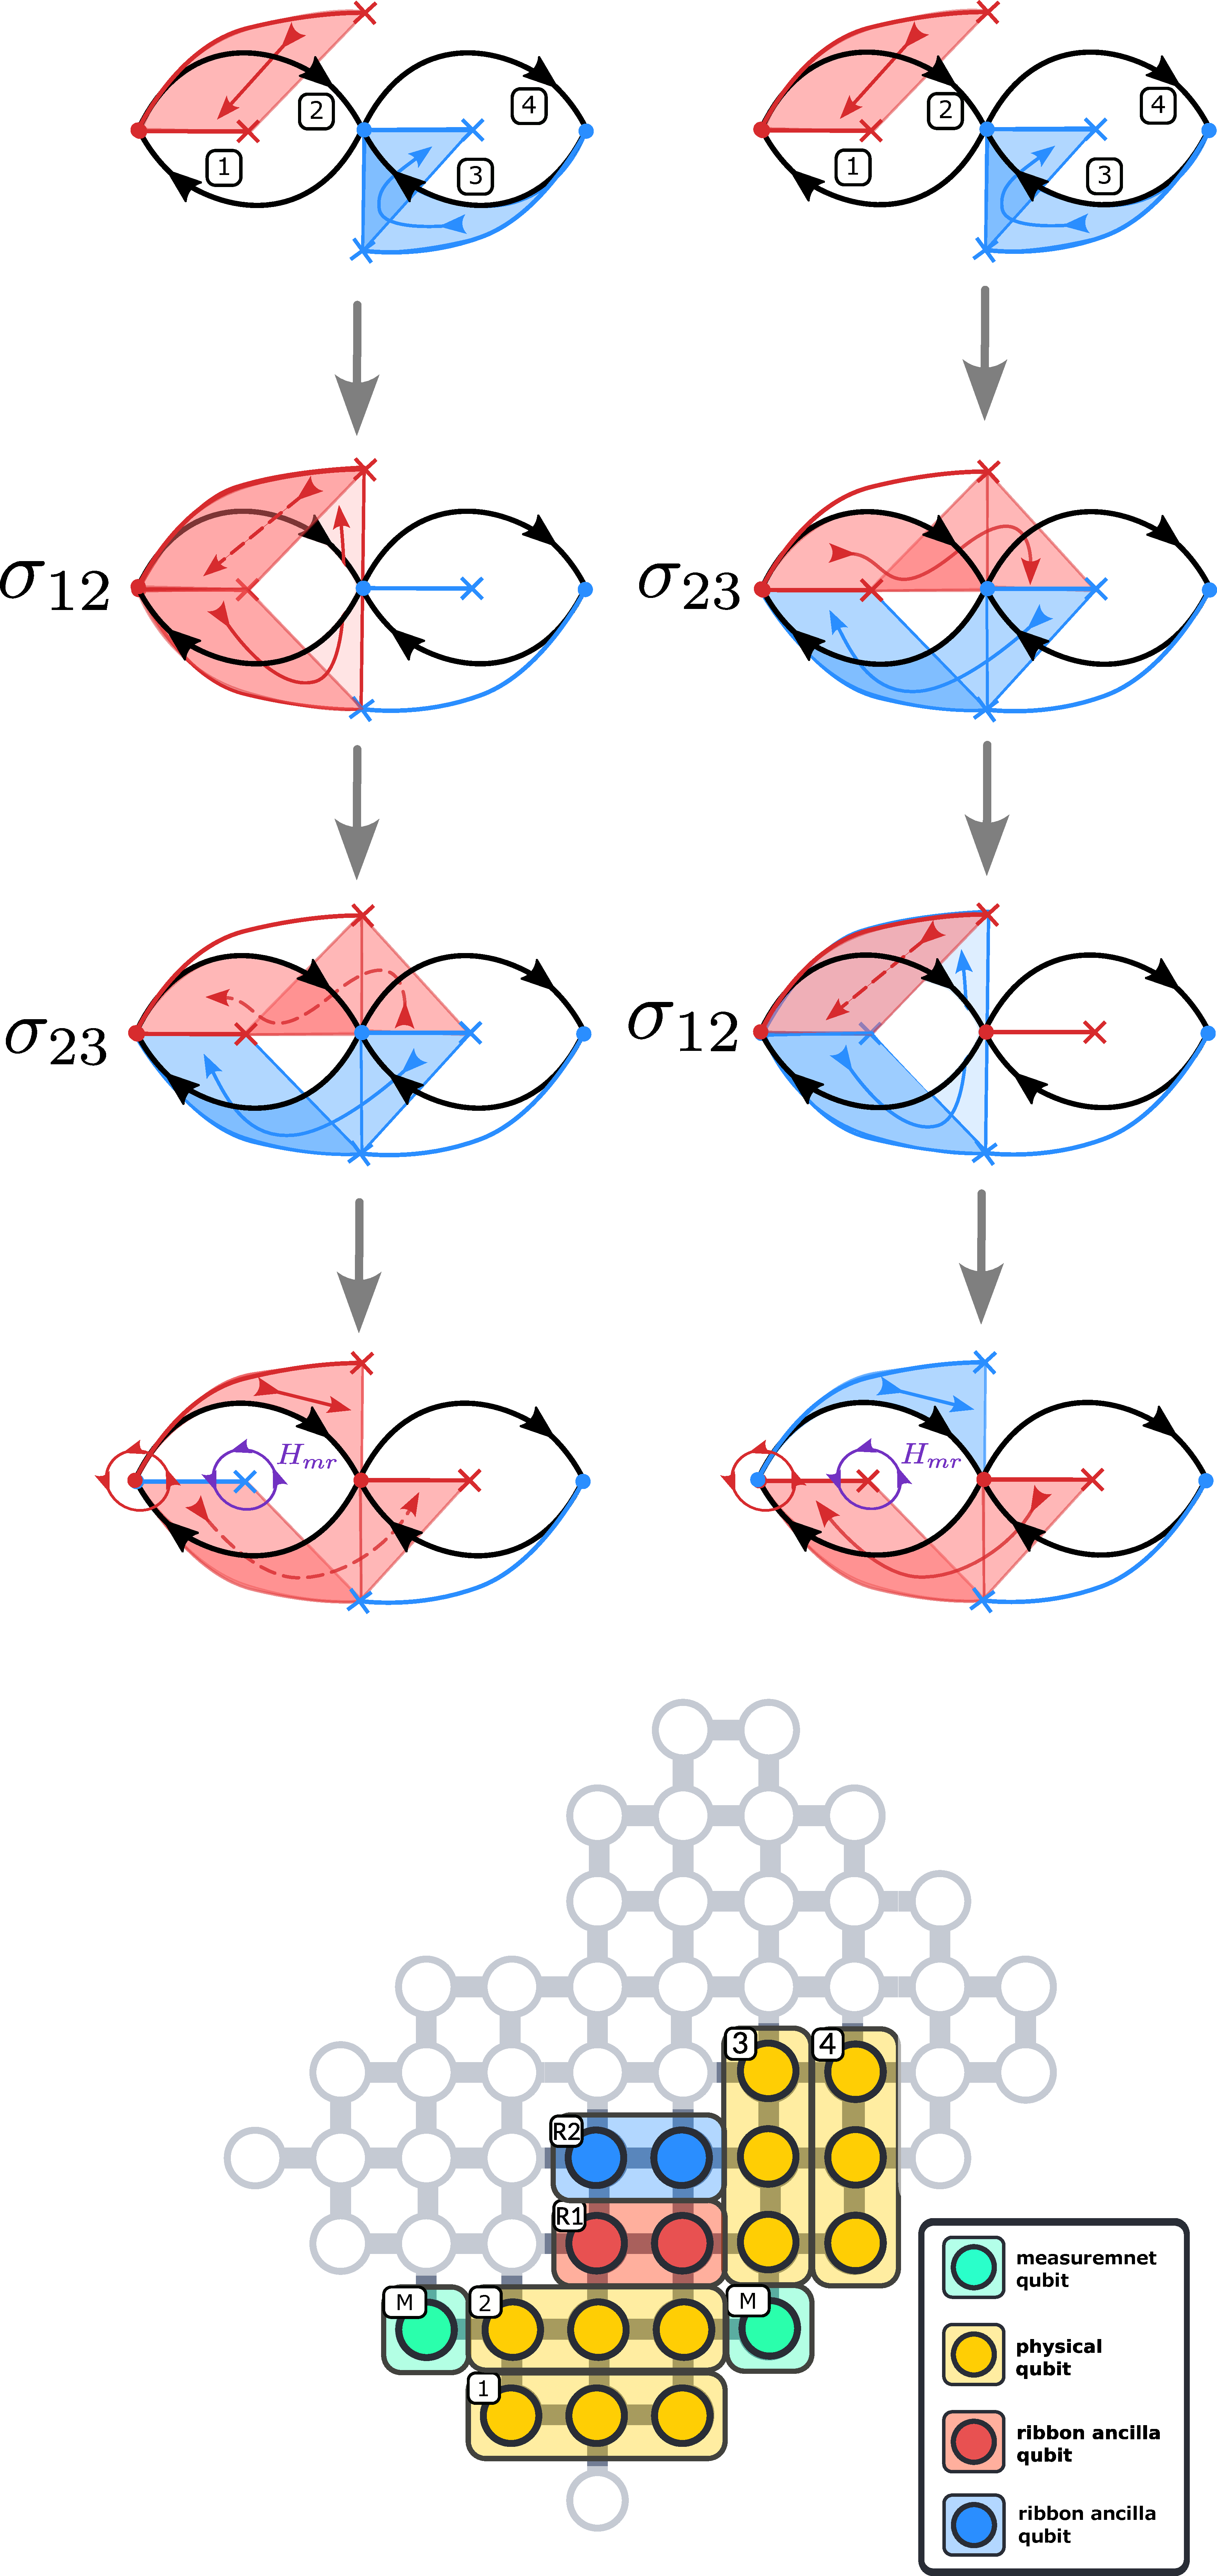
\includegraphics[width=\linewidth]{Figures/braiding_setup.pdf}
	\caption{(Top) The ribbon operators for the two braiding experiments. On the last step we also label around which plaquette we perform the $H_{mr}$-partial charge measurement. Note that we are on a sphere so the outside plaquette that we labelled twice for clarity should be identified. This is best seen in the diagram for the $\sigma_{12}$-exchange. (Bottom) The circuit layout on the Sycamore chip we used to simulate the braiding experiment.}
	\label{fig:braiding_setup}
\end{figure}

%The circuit depths achieved for braiding the $\Psi_m$ fluxes are 23 and 25 

The circuit depths achieved for braiding the $\Psi_m$ fluxes are 60 and 68 for the cases of $\sigma_{23}\sigma_{12}$ and $\sigma_{12}\sigma_{23}$, respectively. We note that we did these experiments on the double braiding ladder, \caro{making the sites 2 and 3 share the vertex.} This is due to constraints of the simulation. Adding 6 extra qubits needed for a triple-ladder, dramatically slows down the run times to the point of impracticality. On a real quantum device this problem would not occur.

%Once compiled to only use CZ as the two-qubit gate we get 60 and 68 for the two cases respectively.

\emph{Ground state.} As mentioned, we prepare the ground state directly. On the braiding ladder that procedure is depth 2. We prepare the qubits on all the bottom edges in an equal superposition via Hadamard gates and then CNOT the qubits above controlled by the one below. 

On the planar graph in Figure \ref{fig:basketball} this process is more complicated. Repeating the process as for the braiding ladder gives us the following state $\ket{\Psi} = \sum_{g_{12},g_{34}}\ket{g_{12},g_{12}, g_{34}, g_{34}}$. We then apply the full controlled multiply circuit from qubits of the second edge onto the qubits of the third edge. This procedure gives us the state defined in Figure \ref{fig:basketball}, up to a simple relabelling\caro{what relabelling?}.

\textbf{Results.}
The results of the fusion experiments on the ladder and the planar graph, as well as the braiding on the ladder are shown in Figure \ref{fig:red_charge_res}.
\begin{figure*}
\centering
\begin{subfigure}{0.47\textwidth}
    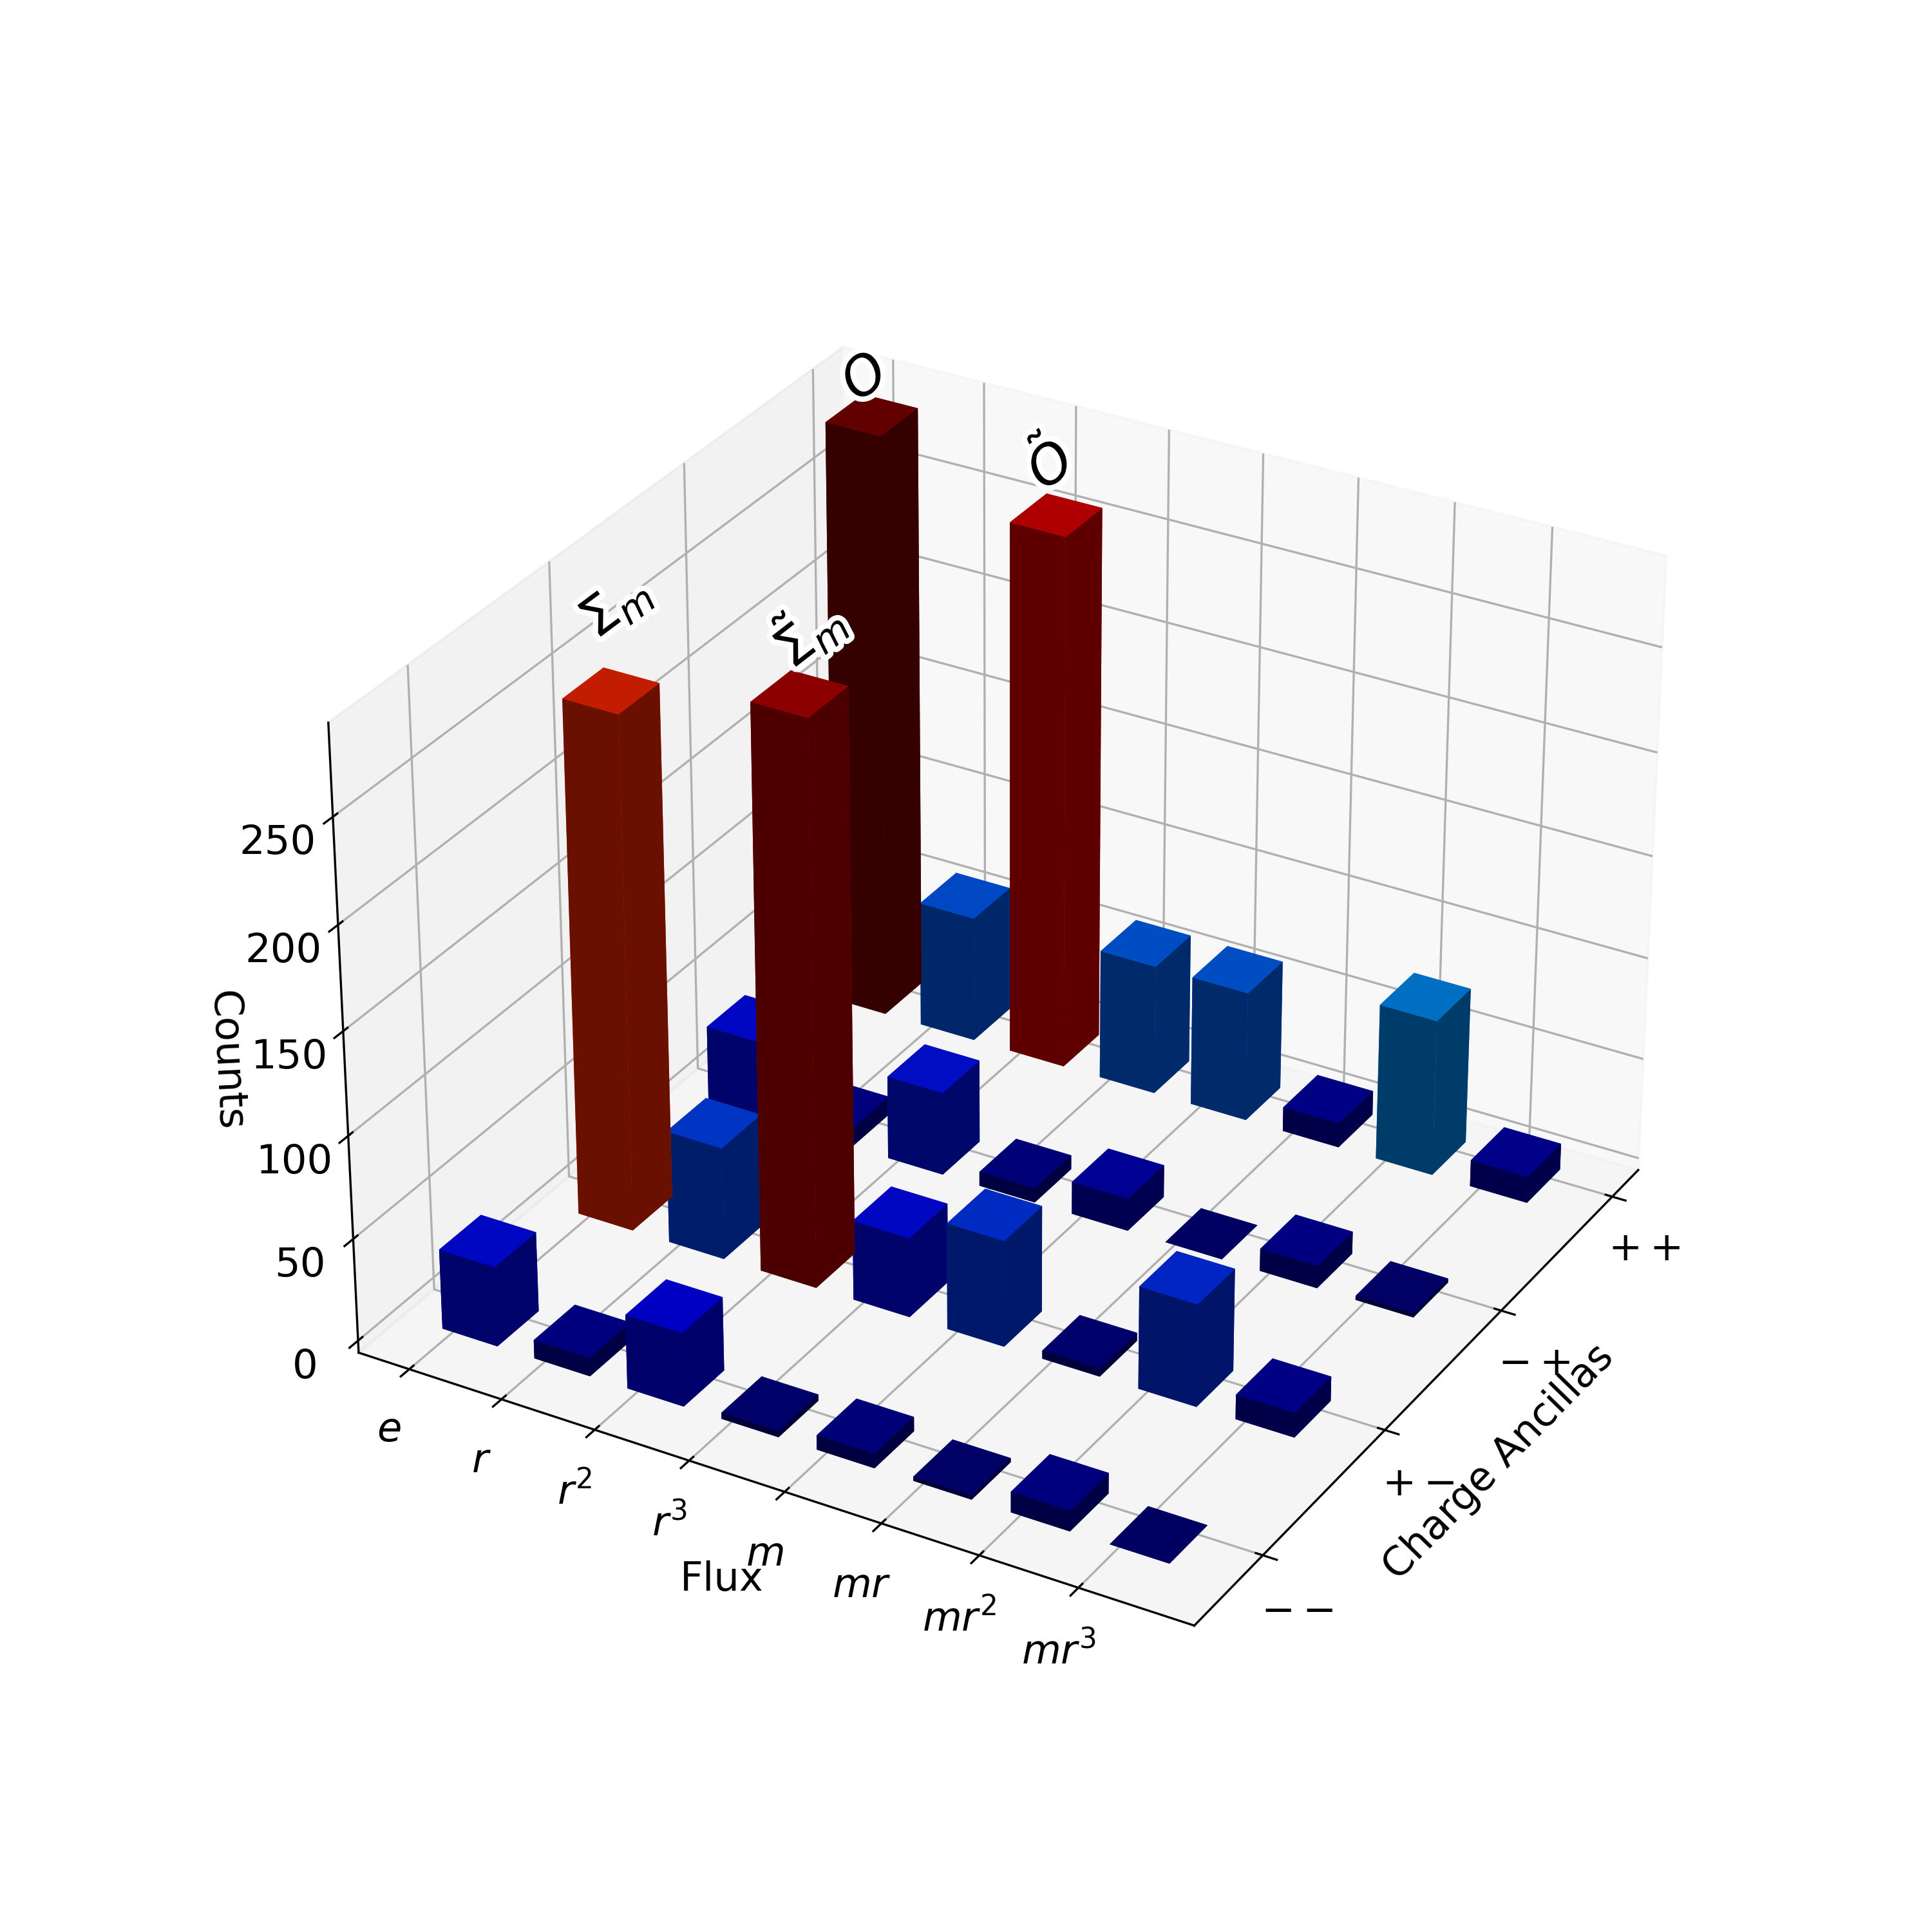
\includegraphics[width = \linewidth]{Figures/fusion_on_glasses.png}
    \caption{The reduced charge-flux measurement after fusing two $\Psi_m$ pure fluxes on the site of fusion. The reduced charge was done with $H_{mr}$ subgroup, and the geometry was that of the braiding ladder, Figure \ref{fig:latticeGS}.}
    \label{fig:fusion_glass}
\end{subfigure}\hfill
\begin{subfigure}{0.47\textwidth}
    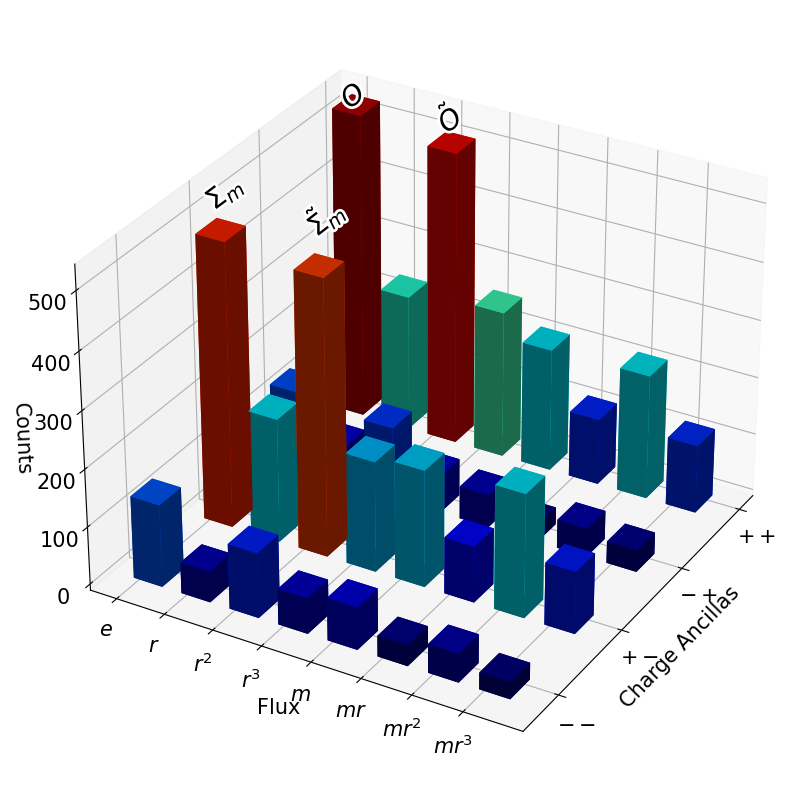
\includegraphics[width=\linewidth]{Figures/fusion_on_basketball.png}
    \caption{The reduced charge-flux measurement after fusing two $\Psi_m$ pure fluxes on the site of fusion. The reduced charge was done with $H_{mr}$ subgroup, and the geometry was that of the small two-dimensional graph, Figure \ref{fig:basketball}.}
    \label{fig:fusion_basketball}
\end{subfigure}
\vspace{15pt}
\begin{subfigure}{0.47\textwidth}
    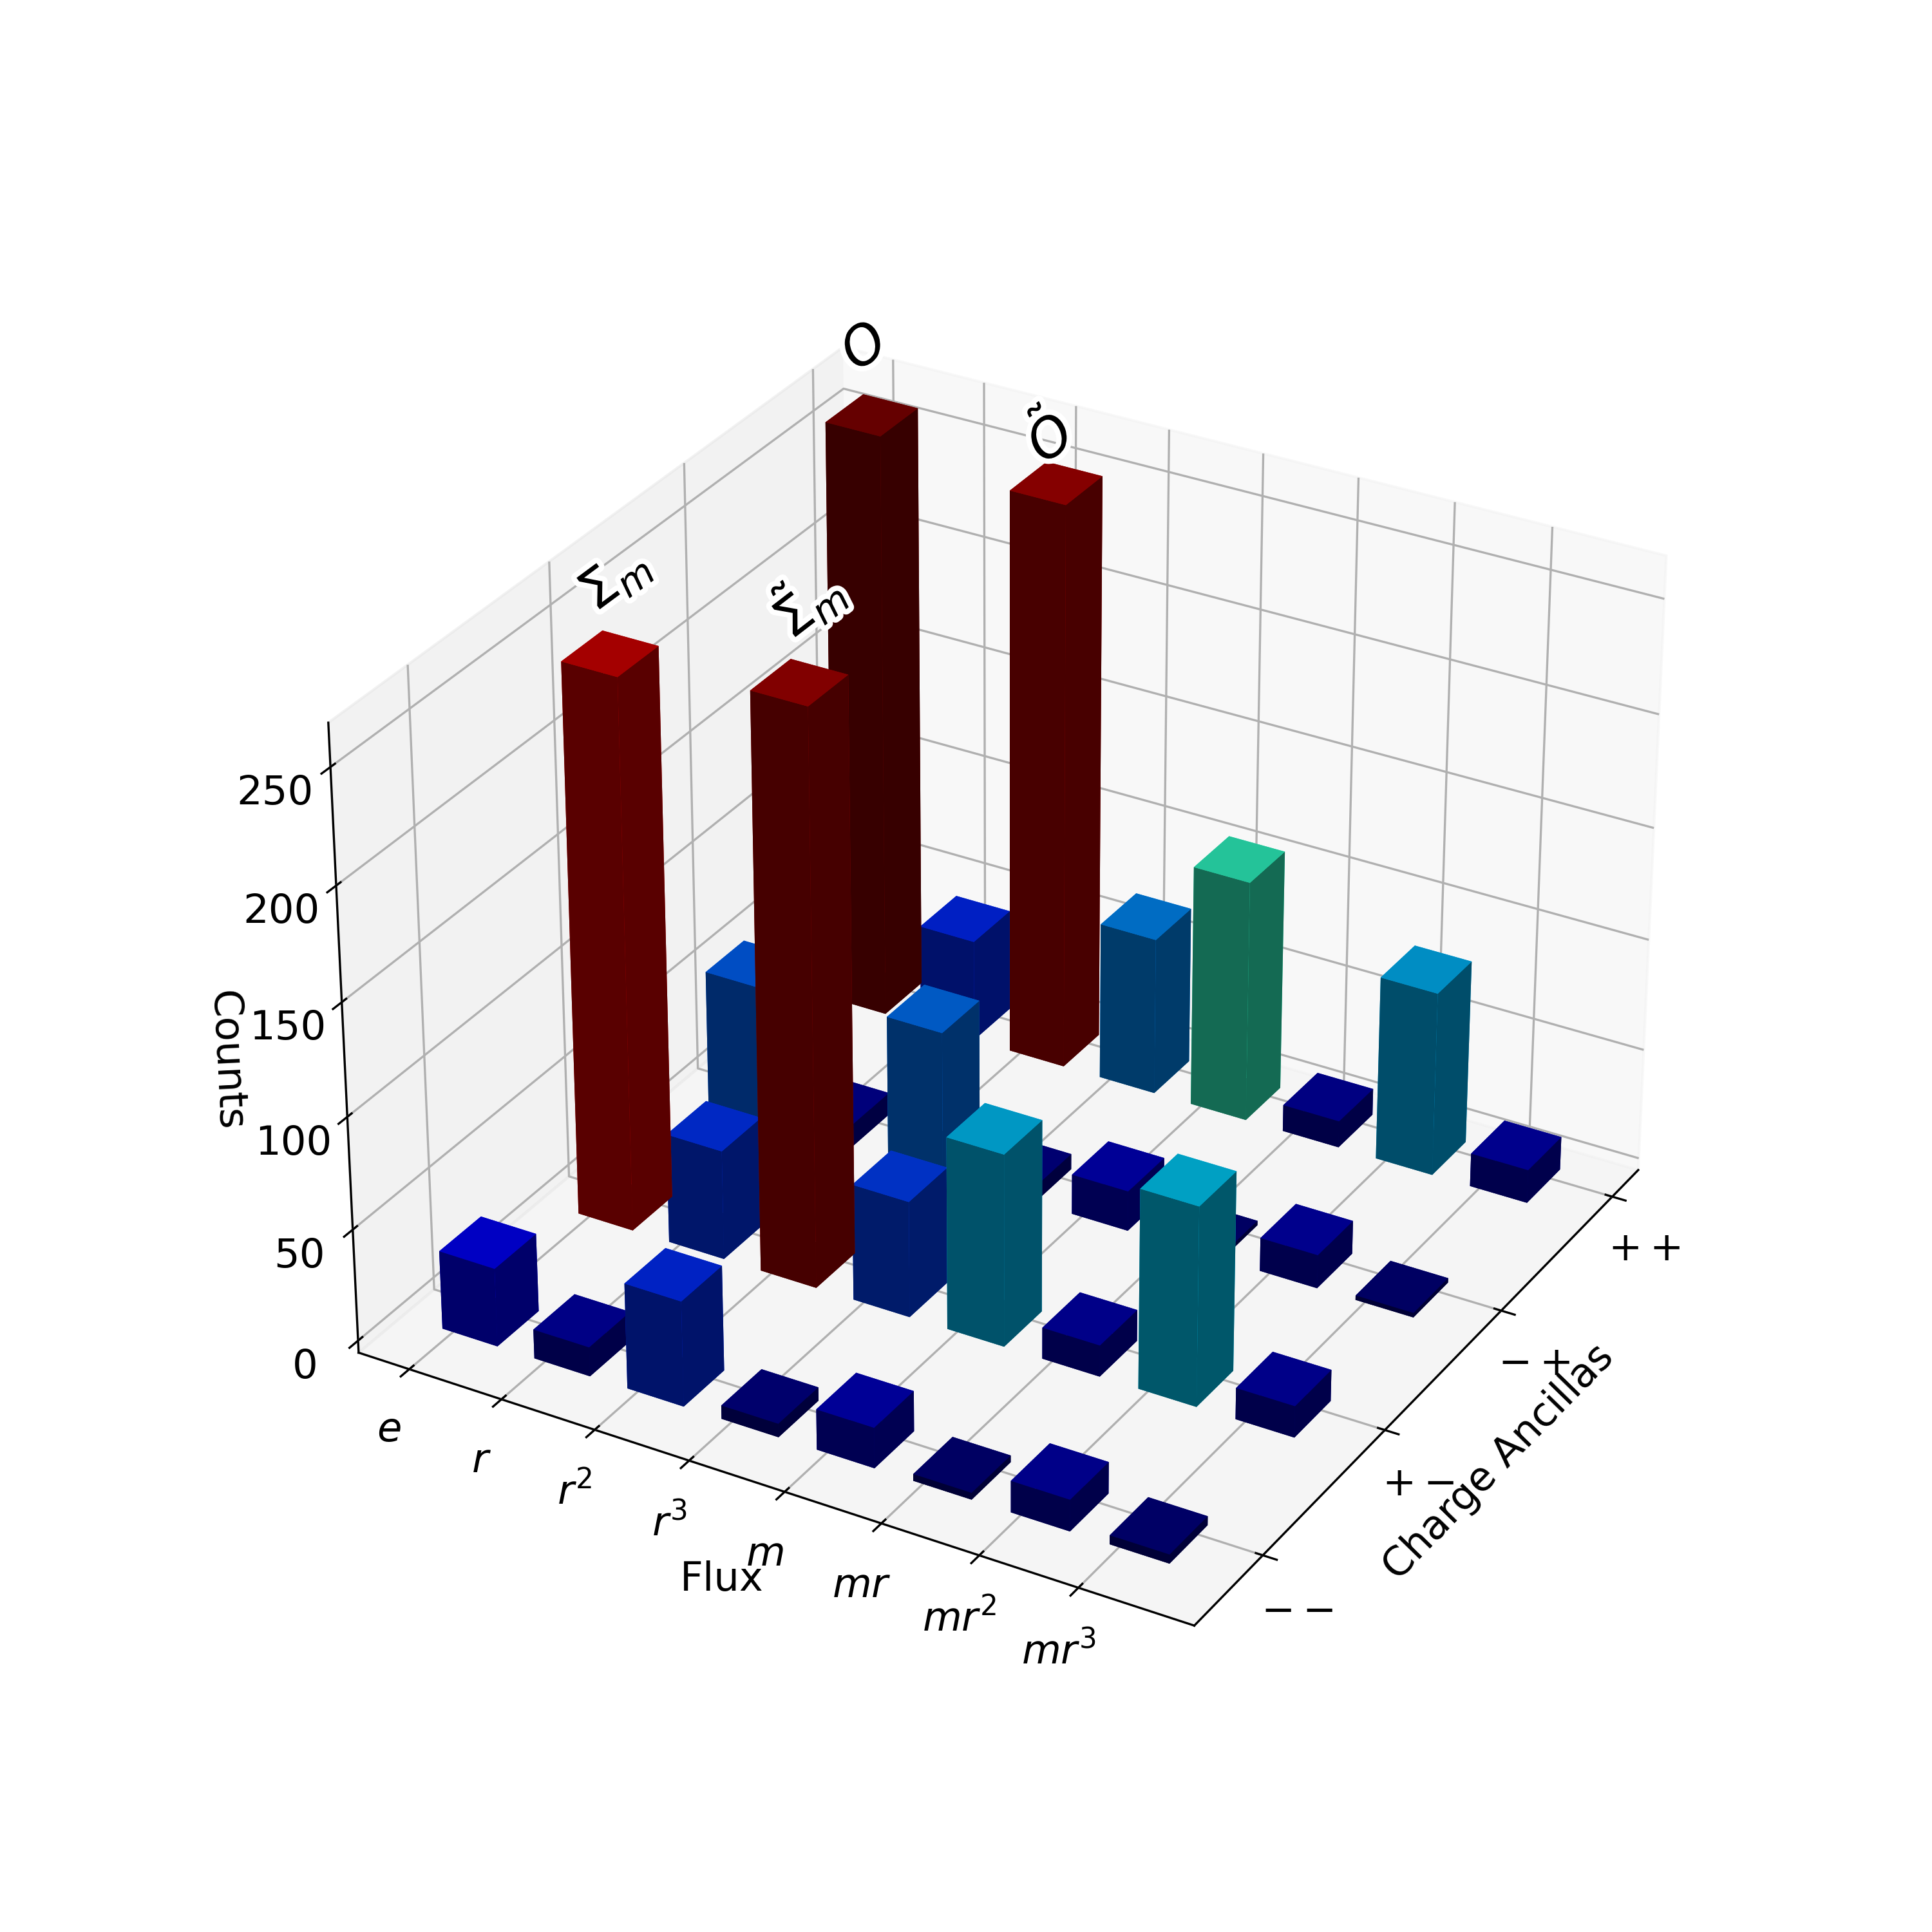
\includegraphics[width=\linewidth]{Figures/braid_fusion.png}
    \caption{The braiding on a braiding ladder: the reduced charge-flux measurement after performing the braiding protocol in $\sigma_{12}\sigma_{23}$ order, Figure \ref{fig:flux_braid} (left), where $\sigma_{ii+1}$ is a braid group generator. The anyons used are the pure fluxes $\Psi_m$. The reduced charge measurement was done with respect to $H_{mr}$ subgroup.} 
    \label{fig:braid_fuse}
\end{subfigure}\hfill
\begin{subfigure}{0.47\textwidth}
    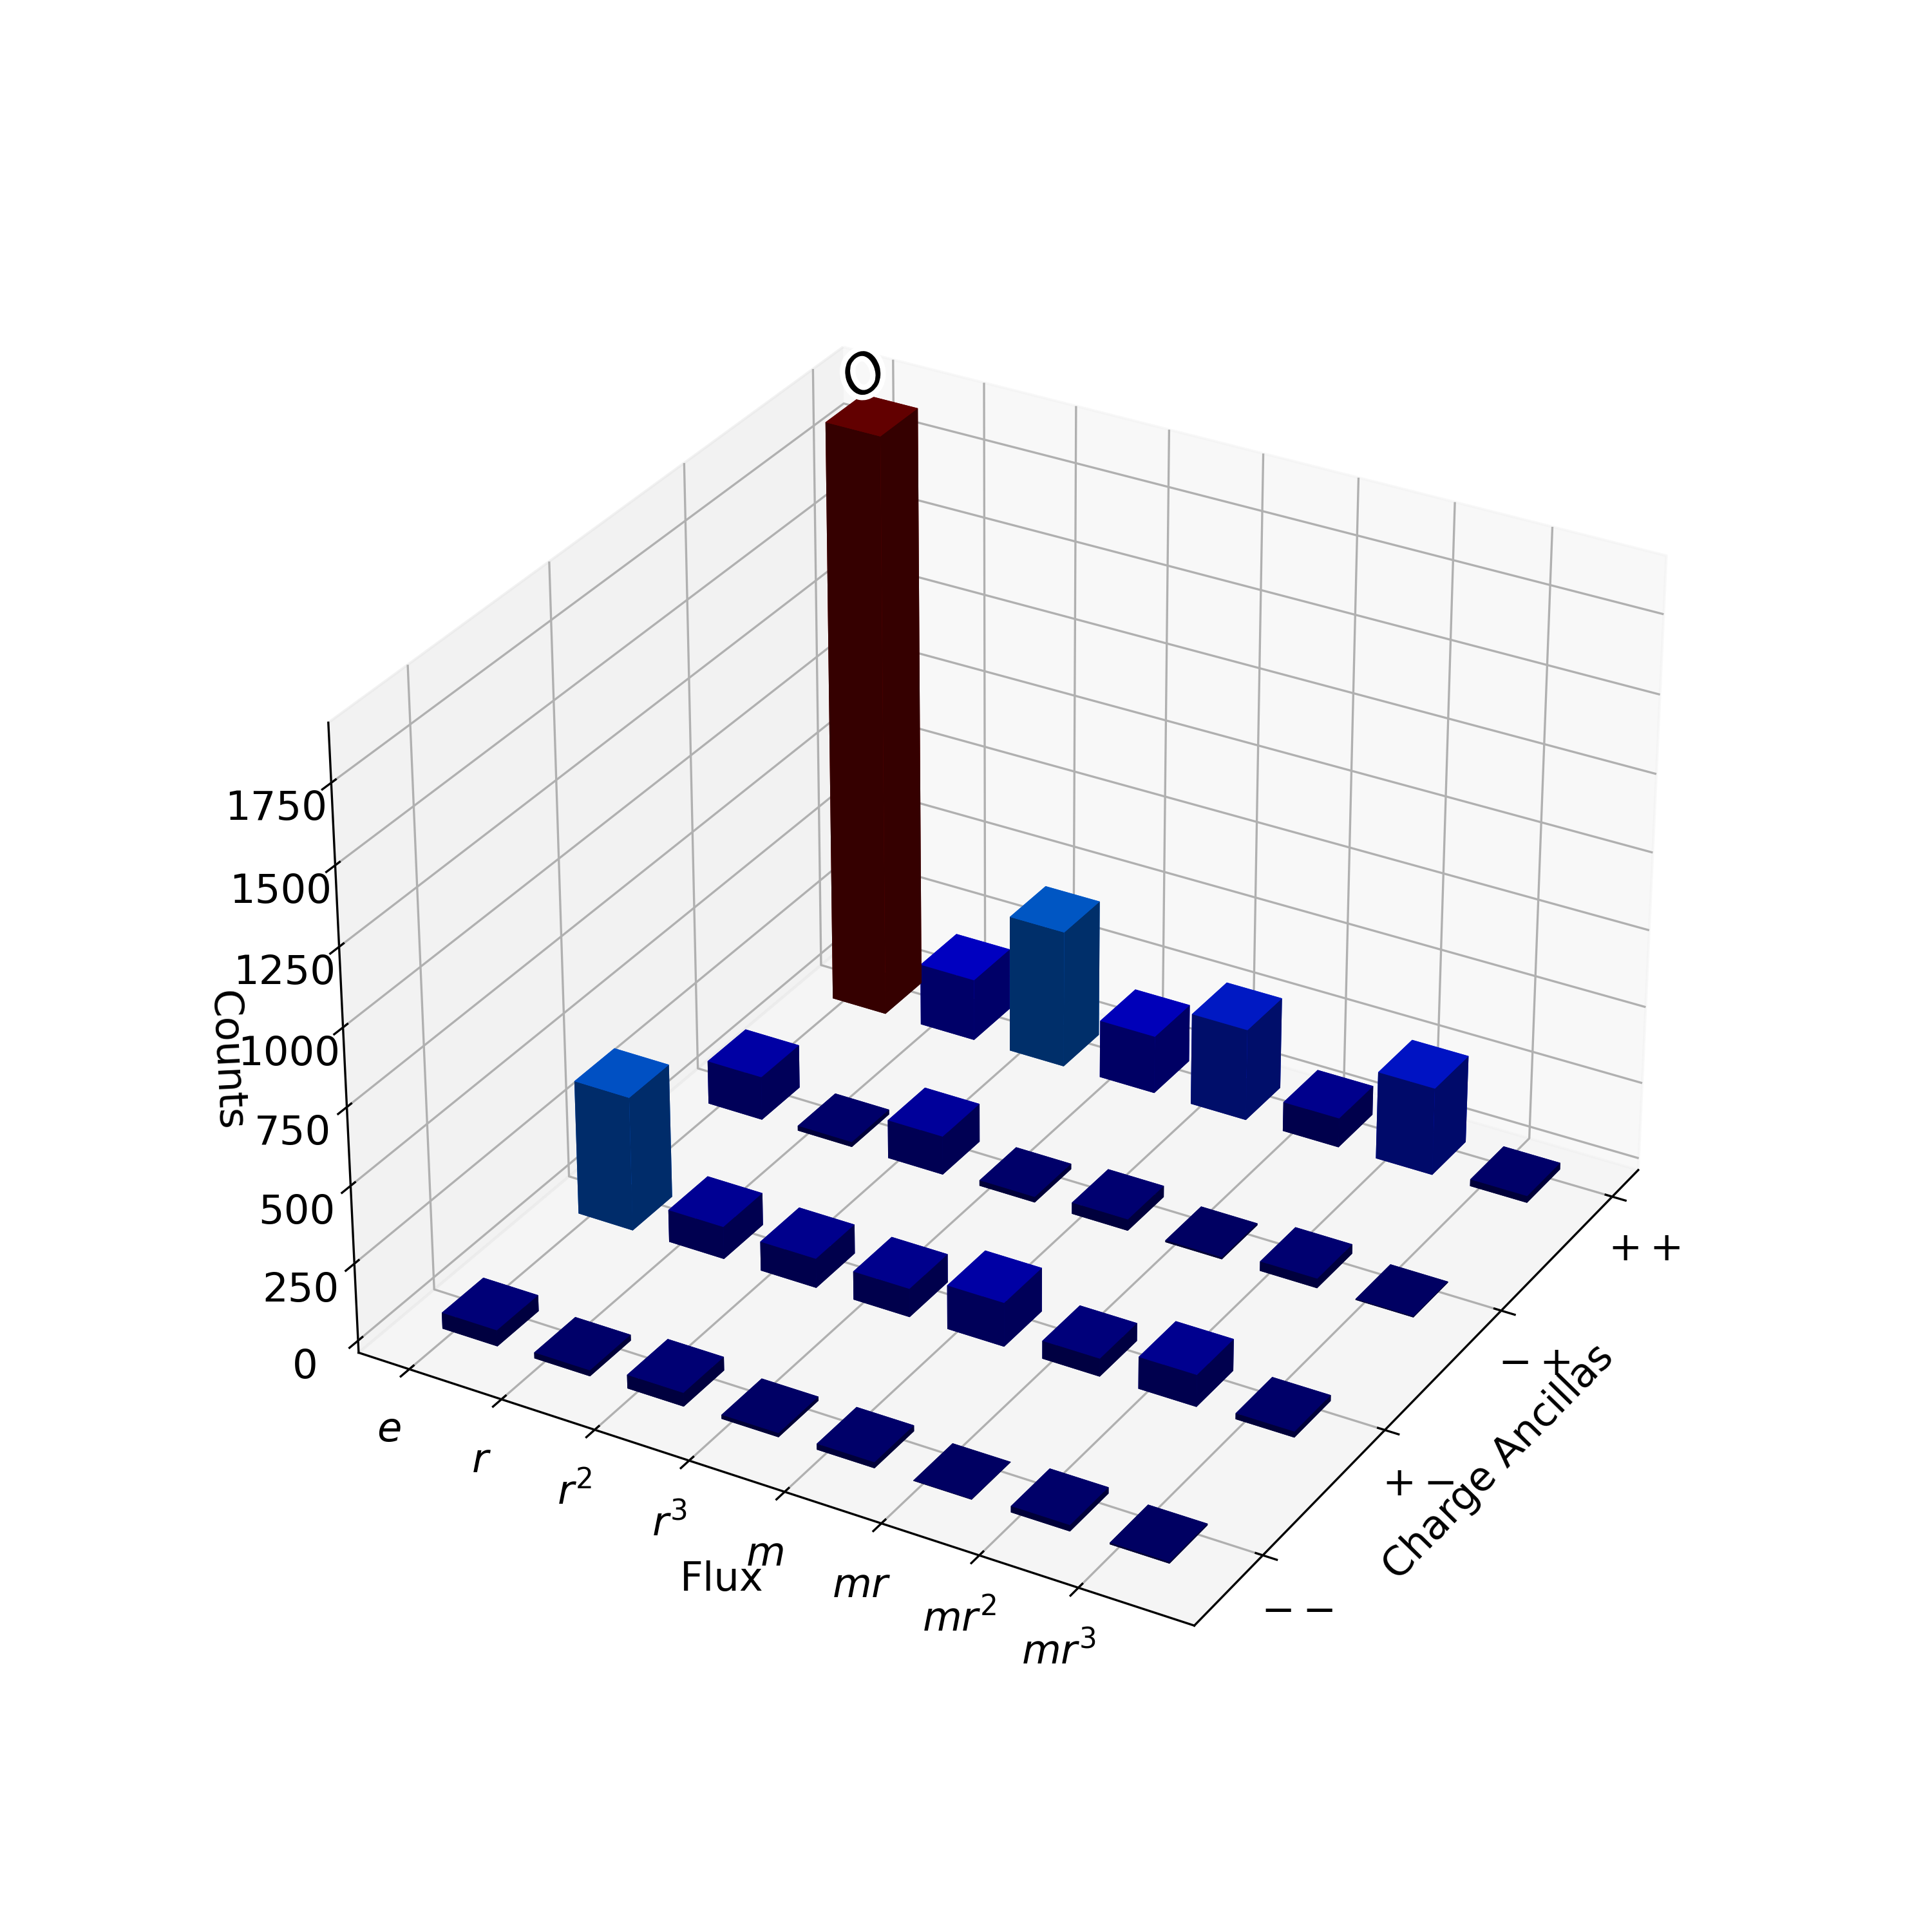
\includegraphics[width=\linewidth]{Figures/braid_link.png}
    \caption{The braiding on a braiding ladder: the reduced charge-flux measurement after performing the braiding protocol in $\sigma_{23}\sigma_{12}$ order, Figure \ref{fig:flux_braid} (right), where $\sigma_{ii+1}$ is a braid group generator. The anyons used are the pure fluxes $\Psi_m$.The reduced charge measurement was done with respect to $H_{mr}$ subgroup.}
    \label{fig:braid_link}
\end{subfigure}
\caption{The reduced topological charge measurements for the fusion and braiding protocols.}
\label{fig:red_charge_res}
\end{figure*}

\emph{Fusion.} 
On both lattices we measure the charge after fusion and see the signatures of four fusion outcomes
$$\Psi_m \otimes \Psi_m = 0 \oplus \tilde 0 \oplus \Sigma_m \oplus \tilde{\Sigma}_m.$$
In the case of the small planar graph we see a significantly 
increased background noise due the deeper circuit used in the ground state preparation.

%while the actual number of successes was $1807$, 
The number of runs for the fusion on the braiding ladder was $16000$. The expected post-selection probability for the projection of the two ribbon ancilla pairs is $1/4^2=0.0625$, while the actual rate of success was $0.113$, due to the circuit noise and measurement readout bias. The four main bins count $270(16)$ with the biggest noise peak being $77(8)$. \caro{what do the numbers in brackets mean?}

The number of runs for the fusion on the small planar graph was $64000$. The expected post-selection probability for projection of the two ribbon ancilla pairs is again $0.0625$, while the actual number of successes was $0.0826$. The four main bins count $450(20)$ with the biggest noise peak being $242(15)$.

\emph{Braiding.}
Looking at the results of the charge measurement for the two braiding protocols we clearly see what we expected. The first braiding protocol results in multiple fusion outcomes while for the second braiding protocol the resulting fusion outcome is only vacuum.


The number of runs for both protocol was $16000$. The expected post-selection probabilities for the two protocols are $1/16$ for $\sigma_{12}\sigma_{23}$ and $1/2$ for $\sigma_{23}\sigma_{12}$, while the actual rates of successes were $0.123$ for $\sigma_{12}\sigma_{23}$ and $0.315$ for $\sigma_{23}\sigma_{12}$, respectively.
%while the actual number of successes was $1977$ for $\sigma_{12}\sigma_{23}$ and $5036$ for $\sigma_{23}\sigma_{12}$, due to the circuit noise and measurement readout bias.
\caro{why 1/2?}

In the case of the first braiding we see the four main peaks counting 255(16) with the biggest peak coming from the noise counting 109(10). In the second case the peak corresponding to the vacuum counts 1890(40) with the largest peak coming from the noise counting 450(20).

For the detailed discussion of the post-selection probabilities see Appendix \ref{app:postsel}.
\caro{comment on other anyons? repeated partial charge measurement? how about we just state values of bins individually and then give a signal to noise ratio.}


\subsection{Linking and Twist Matrices}

In this section, we present the results of our simulations of our interference protocols for measuring the magnitude and the phase of the $S-$ and $T-$matrix elements. 

\textbf{Interference and Tomography.}
\caro{Need to discuss that we are dealing with a mixed state and that we have entanglement between control and gauge field bc of errors}

In Section \ref{subsec:Intef}, we have proposed an interference scheme that entangles an auxiliary qubit with the space-time history of the gauge field excitations, in such a way that by the end of the protocol the qubit and the field are disentangled and the qubit is left in a state that depends only on the topological properties of the said spacetime history of the anyons, the $S-$ and $T-$matrix elements.

The fact that the qubit is meant to be disentangled from the gauge field and any additional ancillas implies that the qubit is ideally left in a pure state, hence easy to tomograph and extract the aforementioned topological properties.  

However the noise in the gates alone will, in addition to decohering the full many-qubit state, result in the final state still being entangled with the gauge field, hence the single qubit state of the auxiliary qubit will be a mixed density matrix
\begin{equation}
    \rho_c = \frac{\mathbb{1} + \vec{r} \cdot \vec{\sigma}}{2},
\end{equation}
where $\vec{r}$ is the Bloch vector and $\vec{\sigma} = (\sigma_x, \sigma_y, \sigma_z)$ is the vector of Pauli matrices. The Bloch vector lives inside a unit sphere, $|\vec{r}|< 1$.

If the state was pure the length of the Bloch vector would be unity.

It is here where we assume that the noise will only shorten the Bloch vector, which is a strong assumption given that the generic dephasing process usually pulls the Bloch vector towards the Z-axis. This is done in order to make the problem tractable without additional machine specific information.

We assume this because it is the direction of the Bloch vector that encodes the result of the interference protocol, the magnitude and the phase of the measured matrix element.


The final pure state of the auxiliary qubit after the ideal protocol is
\begin{equation}
\begin{split}
    \ket{\psi}_c = \frac{1}{\sqrt{1+|\tilde{S}_{ab}|^2}}(\ket{0}_c + \tilde{S}_{ab}\ket{1}_c),\\
    \rho_c = \frac{1}{1+|\tilde{S}_{ab}|^2}\begin{pmatrix}
    1 & \tilde{S}_{ab}^* \\
    \tilde{S}_{ab} & |\tilde{S}_{ab}|^2
    \end{pmatrix},
\end{split}
\end{equation}
which once projected onto the Pauli basis gives us our Bloch vector components: $r_i = \text{Tr}(\sigma_i\rho_c)$,
\begin{equation}
    \vec{r} = \left( \frac{2 \text{Re}\tilde{S}_{ab}}{1+|\tilde{S}_{ab}|^2}, \frac{2 \text{Im}\tilde{S}_{ab}}{1+|\tilde{S}_{ab}|^2}, \frac{1 - |\tilde{S}_{ab}|^2}{1+|\tilde{S}_{ab}|^2} \right).\label{eqn:bloch}
\end{equation}

Note that $|\vec{r}| = 1$ as expected for the pure state and the only relevant parameter for our measurement is the orientation of the Bloch vector. 

\emph{Tomography.} In order to determine the orientation of the Bloch vector we measure in a set of different bases. Each basis is parametrised by a vector $\vec{s}_i$ with $\sigma_{s_i} = \vec{s}_i \cdot \vec{\sigma}$ being the associated Hermitian operator.

Given a basis $\vec{s}_i$ and a Bloch vector of a mixed state $\vec{r}$, the quantum mechanical probabilities for the two measurement outcomes are
$$p_{QM}(1|\vec{s}_i, \vec{r}) = \frac{1}{2}(1+\vec{r}\cdot\vec{s}_i)$$ and 
$$p_{QM}(0|\vec{s}_i, \vec{r}) = \frac{1}{2}(1-\vec{r}\cdot\vec{s}_i).$$

This probability is, however, modulate by the readout bias:
\begin{equation}
    p(b|\vec{s}_i, \vec{r}) = (1-\epsilon_b)p_{QM}(b|\vec{s}_i, \vec{r}) + \epsilon_{\bar{b}} p_{QM}(\bar{b}|\vec{s}_i, \vec{r}), \label{eqn:marg}
\end{equation}
where $\epsilon_b$ is the probability to measure the qubit in state $\bar{b}$ ($\equiv 1-b$) even though it is in the state $b$, these values are known through calibration \cite{}.

Unfortunately, the picture is further complicated by the fact that we do not trace out the additional ancillas for the ribbon application, but we post-select on their biased measurement outcomes. 
The full analysis of this problem is discussed in Appendix \ref{app:marg}, but the takeaway is that the unwanted entanglement coupled with the post-selection on the biased measurement results manifests nontrivially on our auxiliary qubit tomography, i.e. $$p_{\text{True}}(b) \neq p(b|\vec{s}_i, \vec{r}).$$ For example, we find that the observed readout biases, $\epsilon_b$, depend on the full manybody state. 

We will neglect this effect since it depends on the setup specific details of the noise and biases.

Assuming that $p(b|\vec{s}_i, \vec{r})$ is in fact correct and given a measurement outcome as two counts, $(n_0, n_1)$, summing to the total number of shots, $n_0 + n_1 = N$, we construct the following estimator
\begin{equation}
    P(\vec{s}_i) = \frac{n_1-n_0}{n_1+n_0},
\end{equation}
which we call polarisation.

The estimator is unbiased in a way that 
\begin{equation}
    \lim_{N \rightarrow \infty} \frac{n_1-n_0}{n_1+n_0} = (1-2\bar\epsilon)\vec{s}_i \cdot \vec{r} + \Delta\epsilon,\label{eqn:estim}
\end{equation}
with $\bar\epsilon$ the mean value of two readout biases with their difference being $\Delta\epsilon$ (note: $2\bar\epsilon \geq \Delta\epsilon$).

Repeating the measurements for different bases $\vec{s}_i$ allows us to extract $\vec{r}$, up to a multiplicative constant, by fitting.
Ignoring the aforementioned noise effects then allows us to determine the amplitude and phase of the measured matrix elements from Eq.~\eqref{eqn:bloch}\footnote{With an additional multiplicative constant to fix the length of the Bloch vector to the observed one.}.

For the sake of concreteness we chose the following sets of measurements bases  \begin{enumerate}
    \item \emph{Equatorial Scan.} Fixing the value of the polar angle to $\theta = \pi/2$ we vary the azimuthal angle $\phi \in [0, 2\pi)$. From this scan we extract $\phi_{\text{max}}$ which has the largest polarisation.
    \item \emph{Meridian Scan.} Fixing the value of the azimuthal angle to $\phi = \phi_{\text{max}}$ we scan the polar angle $\theta \in [0, 2\pi)$\footnote{The domain is extended on purpose.} From this scan we extract $\theta_{\text{max}}$ which has the largest polarisation.
\end{enumerate}
The extraction of the relevant angles is done by fitting Eq. \ref{eqn:estim}.
The two angles then fix the value of $\tilde{S}_{ab}$: $$\tilde{S}_{ab} = \sqrt{\frac{1-\cos{\theta_{\text{max}}}}{1+\cos{\theta_{\text{max}}}}}e^{i\phi_{\text{max}}}.$$
Other, two parameters, the amplitude and the offset of the polarization do not convey any physics. The offset determines the difference of the effective readout biases, $\Delta\epsilon$ and the amplitude determines the combination of the mean readout bias and the length of the Bloch vector, $(1-2\bar{\epsilon})|\vec{r}|$.

Everything remains the same for $T_{aa}$.

\emph{Results.}
The numerical results for our interference protocols are shown in Figures \ref{fig:flav_cond_res}, \ref{fig:ex_cond_res} and \ref{fig:t_mat_results}.

\begin{figure*}
    \centering
    \begin{subfigure}{\textwidth}
        \centering
        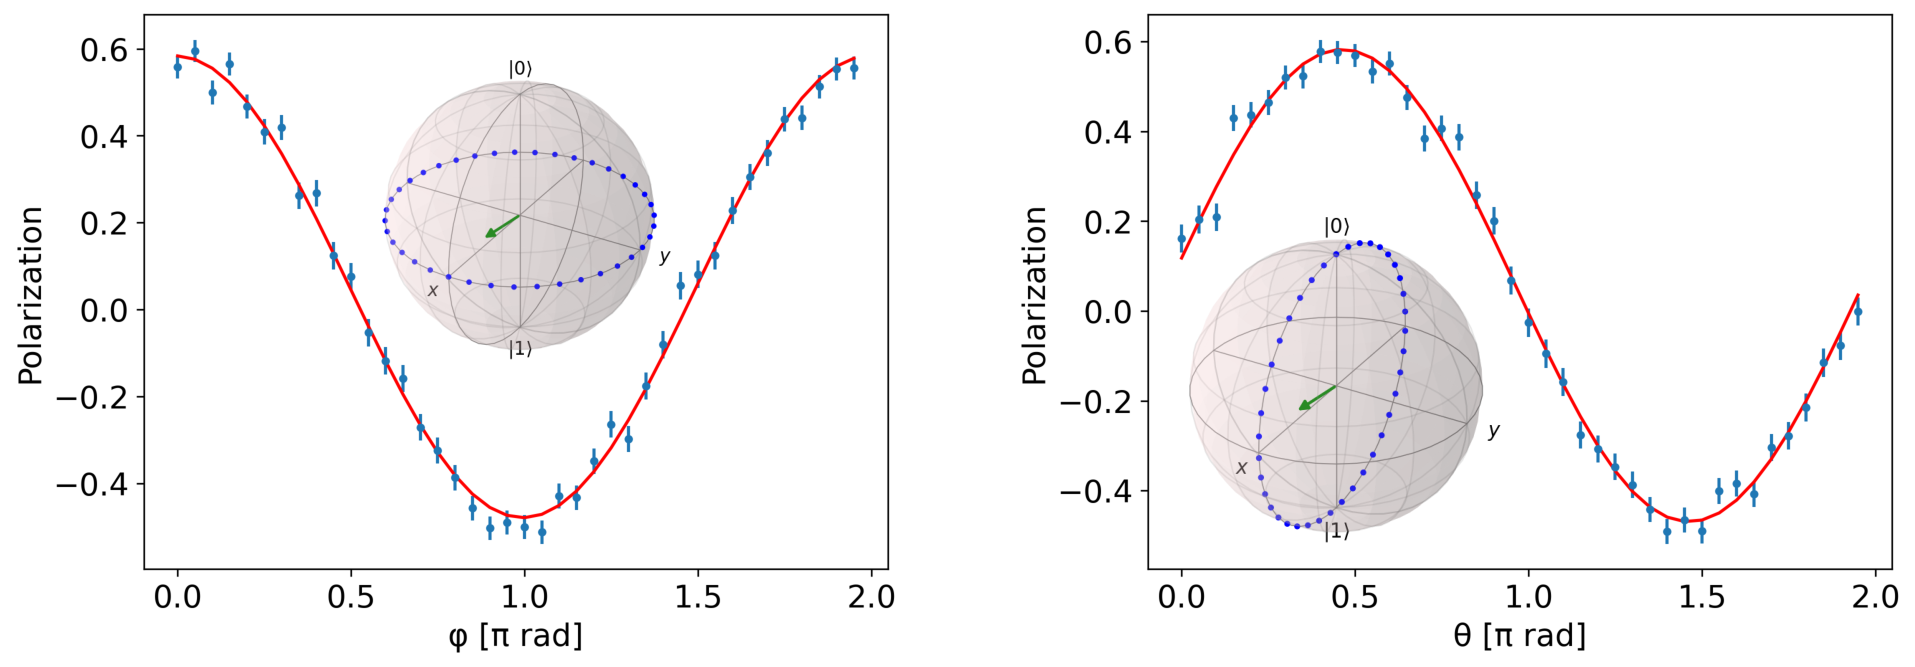
\includegraphics[width=0.85\linewidth]{Figures/flav_s_plus.pdf}
        \caption{The tomography of the control qubit's state after the interference protocol for measuring $S(\Psi_m, \Psi_m) = 1$. The measurement basis was scanned across two planes, see the Bloch sphere diagram (blue dotted circles), and the polarization $P$ was estimated from these measurements, fitting the Eq. \ref{eqn:estim} we have extracted the Bloch vector (orange arrow), from which we have made the estimate: $\tilde{S}(\Psi_m, \Psi_m) = 0.89(1) e^{i\pi 0.004(4)}$. Here the second ribbon's flavour was conditioned, Figure \ref{fig:cond_flav}.}
        \label{fig:flav_cond_res_plus}
    \end{subfigure}
        \begin{subfigure}{\textwidth}
        \centering
        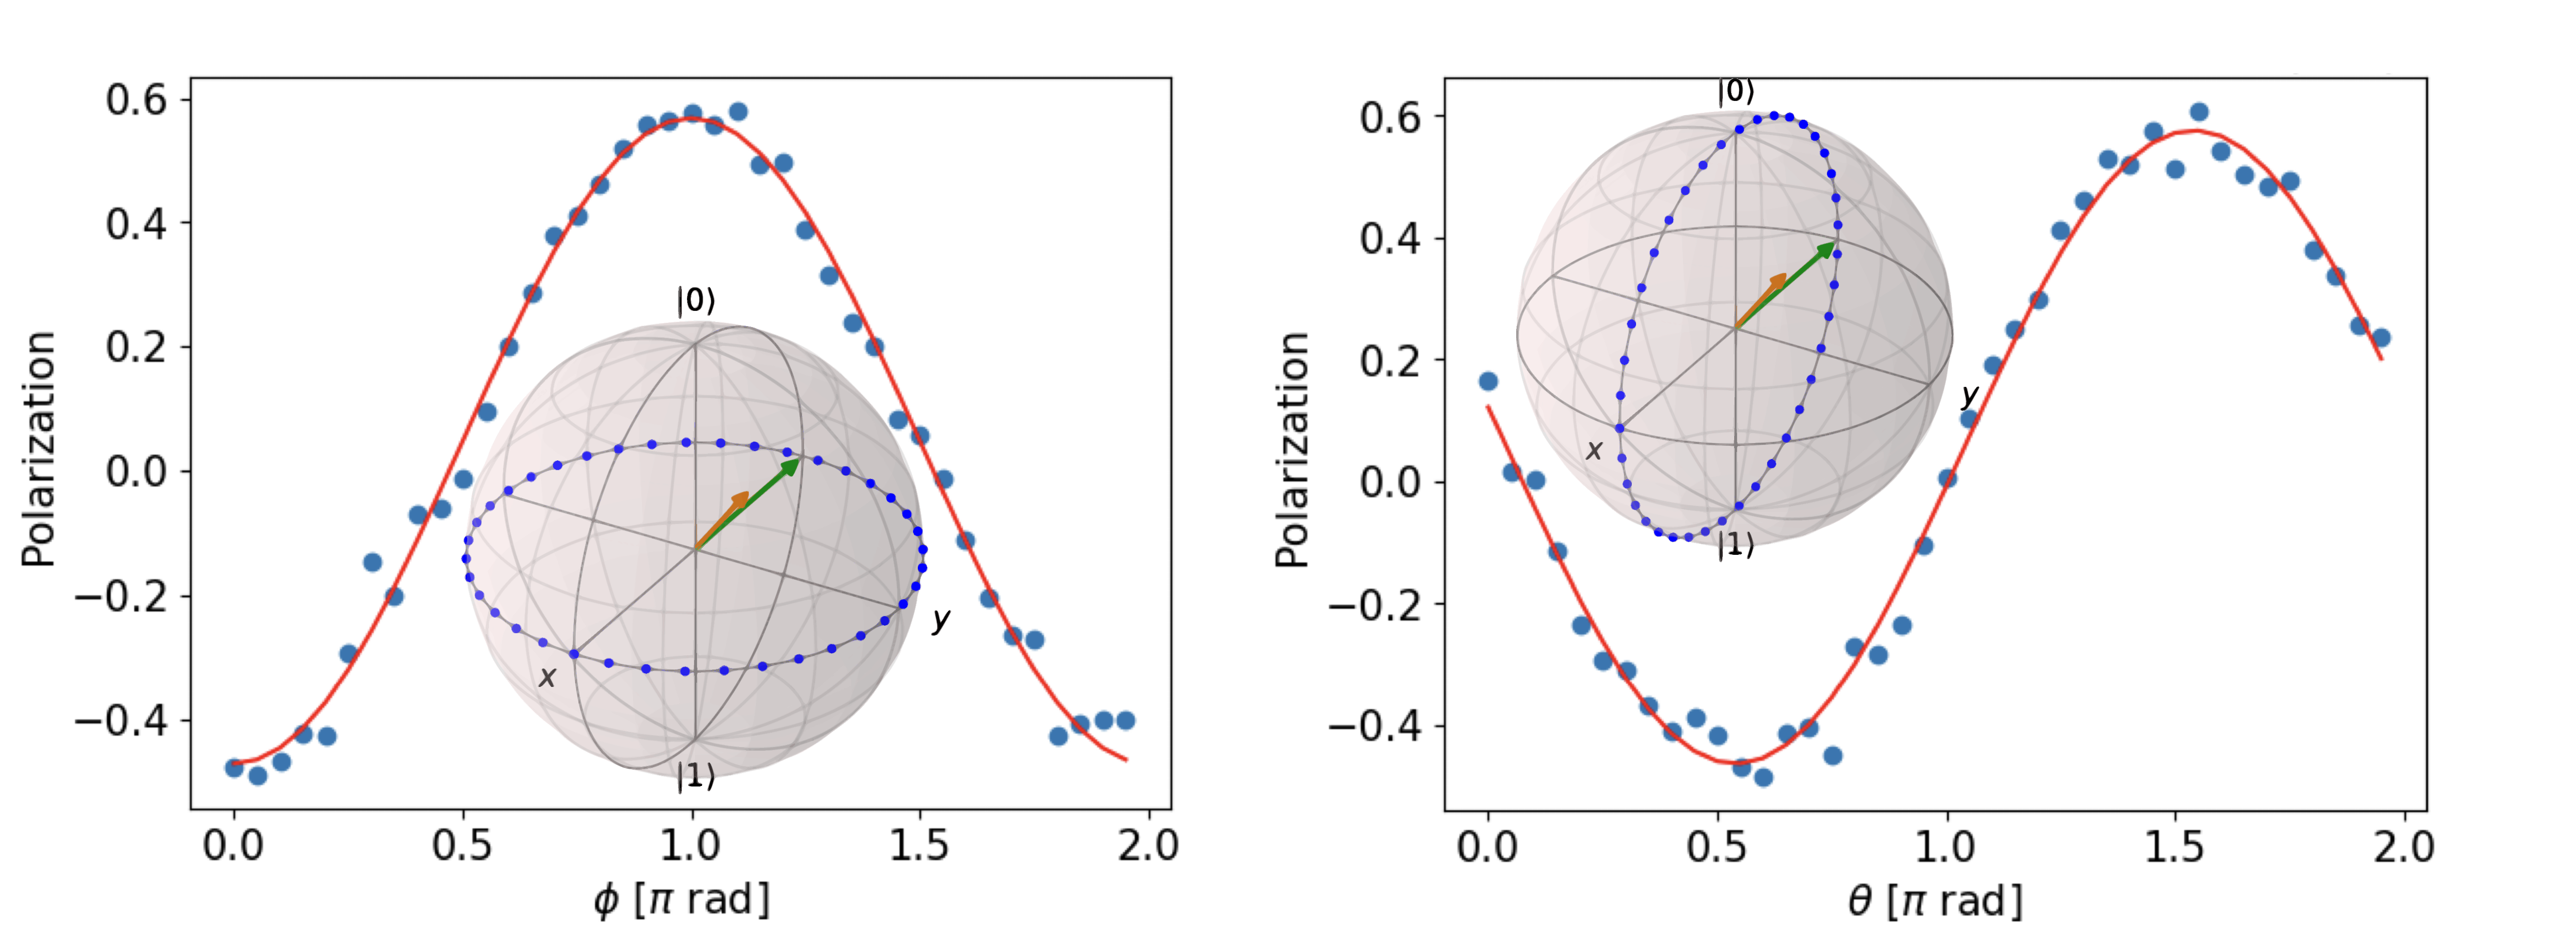
\includegraphics[width=0.8\linewidth]{Figures/flav_s_minus.pdf}
        \caption{The tomography of the control qubit's state after the interference protocol for measuring $S(\Psi_m, \tilde{\Psi}_m) = -1$. The measurement basis was scanned across two planes, see the Bloch sphere diagram (blue dotted circles), and the polarization $P$ was estimated from these measurements, fitting the Eq. \ref{eqn:estim} we have extracted the Bloch vector (orange arrow), from which we have made the estimate: $\tilde{S}(\Psi_m, \tilde{\Psi}_m) = 0.88(1)e^{i\pi 0.998(5)}$. Here the second ribbon's flavour was conditioned, Figure \ref{fig:cond_flav}.}
        \label{fig:flav_cond_res_minus}
    \end{subfigure}
    \begin{subfigure}{\textwidth}
        \centering
        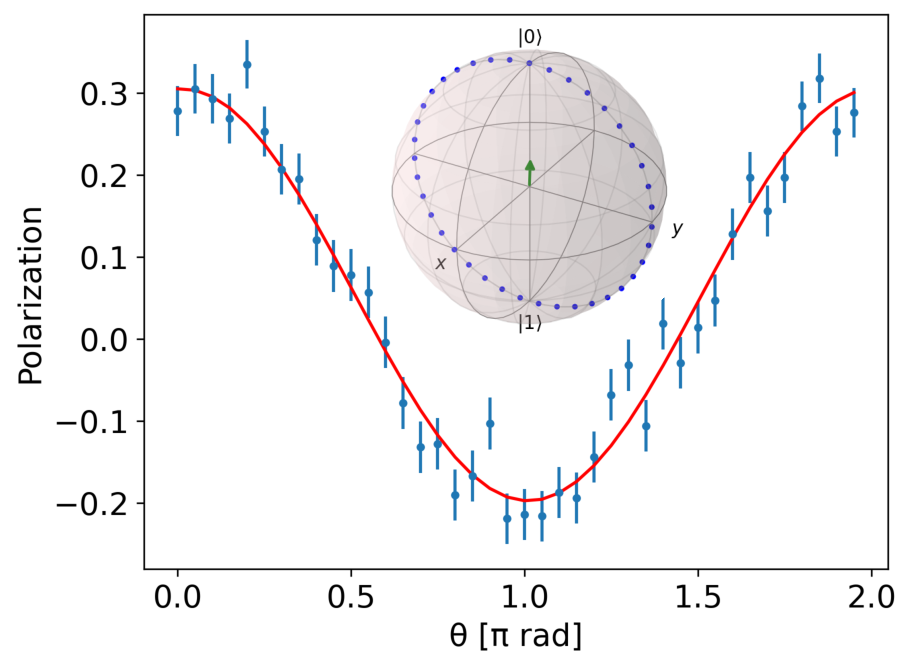
\includegraphics[width=0.4\linewidth]{Figures/flav_s_zero.pdf}
        \caption{The tomography of the control qubit's state after the interference protocol for measuring $S(\Psi_m, \Psi_r) = 0$. The measurement basis was scanned across two planes, see the Bloch sphere diagram (blue dotted circles), and the polarization $P$ was estimated from these measurements, fitting the Eq. \ref{eqn:estim} we have extracted the Bloch vector (orange arrow), from which we have made the estimate: $\tilde{S}(\Psi_m, \Psi_r) = 0.02(2)$. Here the second ribbon's flavour was conditioned, Figure \ref{fig:cond_flav}.}
        \label{fig:flav_cond_res_zero}
    \end{subfigure}
    \caption{Numerical simulation of the S-matrix interference protocol and control qubit tomography.}
    \label{fig:flav_cond_res}
\end{figure*}

\begin{figure*}
        \centering
        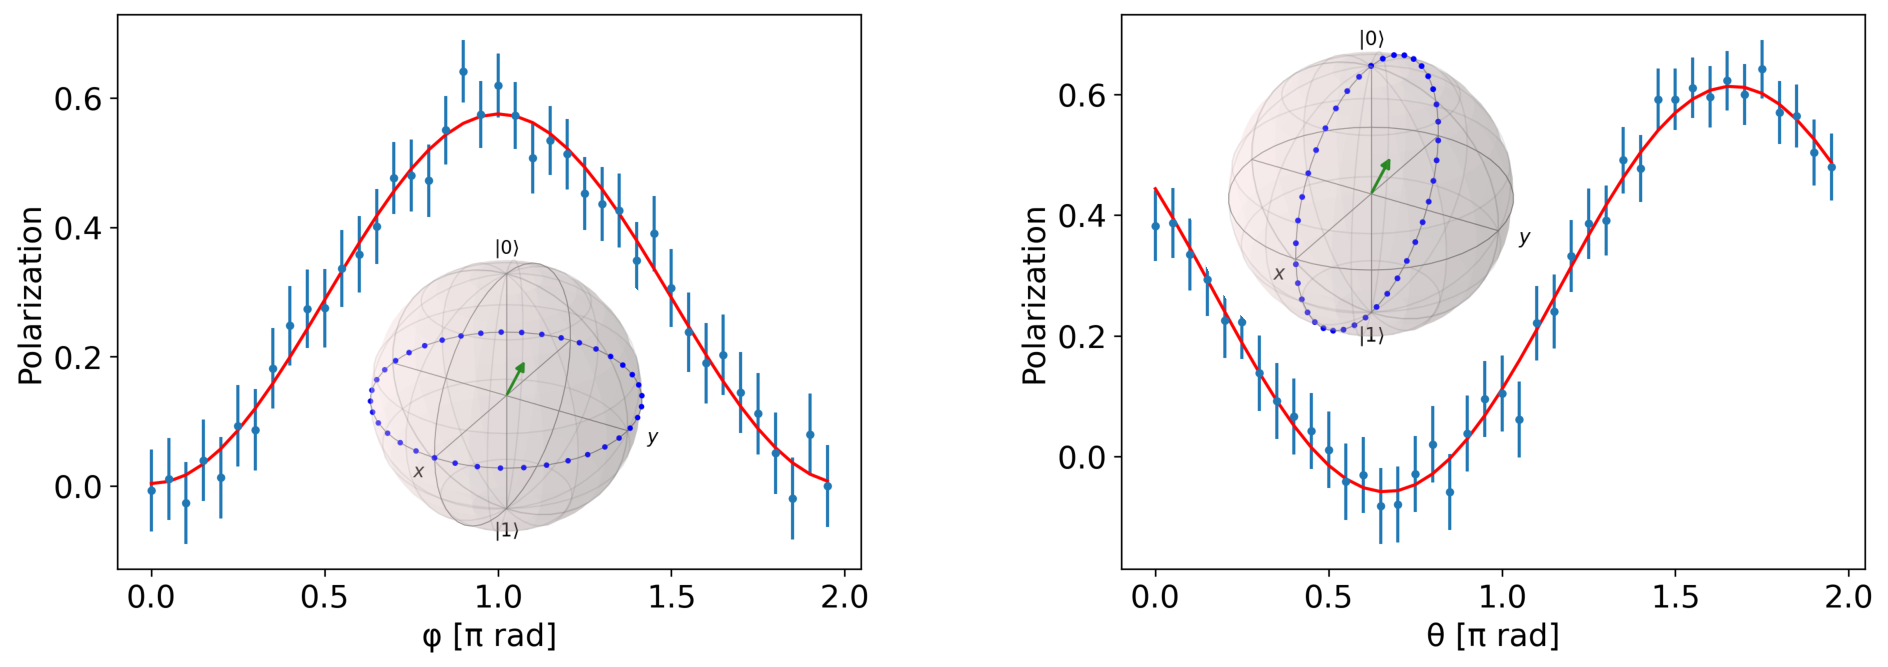
\includegraphics[width=\textwidth]{Figures/exist_s_minus.pdf}
        \caption{Numerical simulation of the S-matrix interference protocol and control qubit tomography: The tomography of the control qubit's state after the interference protocol for measuring $S(\Psi_m, \tilde{\Psi}_m) = -1$. The measurement basis was scanned across two planes, see the Bloch sphere diagram (blue dotted circles), and the polarization $P$ was estimated from these measurements, fitting the Eq. \ref{eqn:estim} we have extracted the Bloch vector (orange arrow), from which we have made the estimate: $\tilde{S}(\Psi_m, \tilde{\Psi}_m) = 0.58(1)e^{i\pi 1.002(8)}$. Here the second ribbon was fully conditioned, Figure \ref{fig:cond_ex}.}
        \label{fig:ex_cond_res}
\end{figure*}

\begin{figure*}
    \centering
    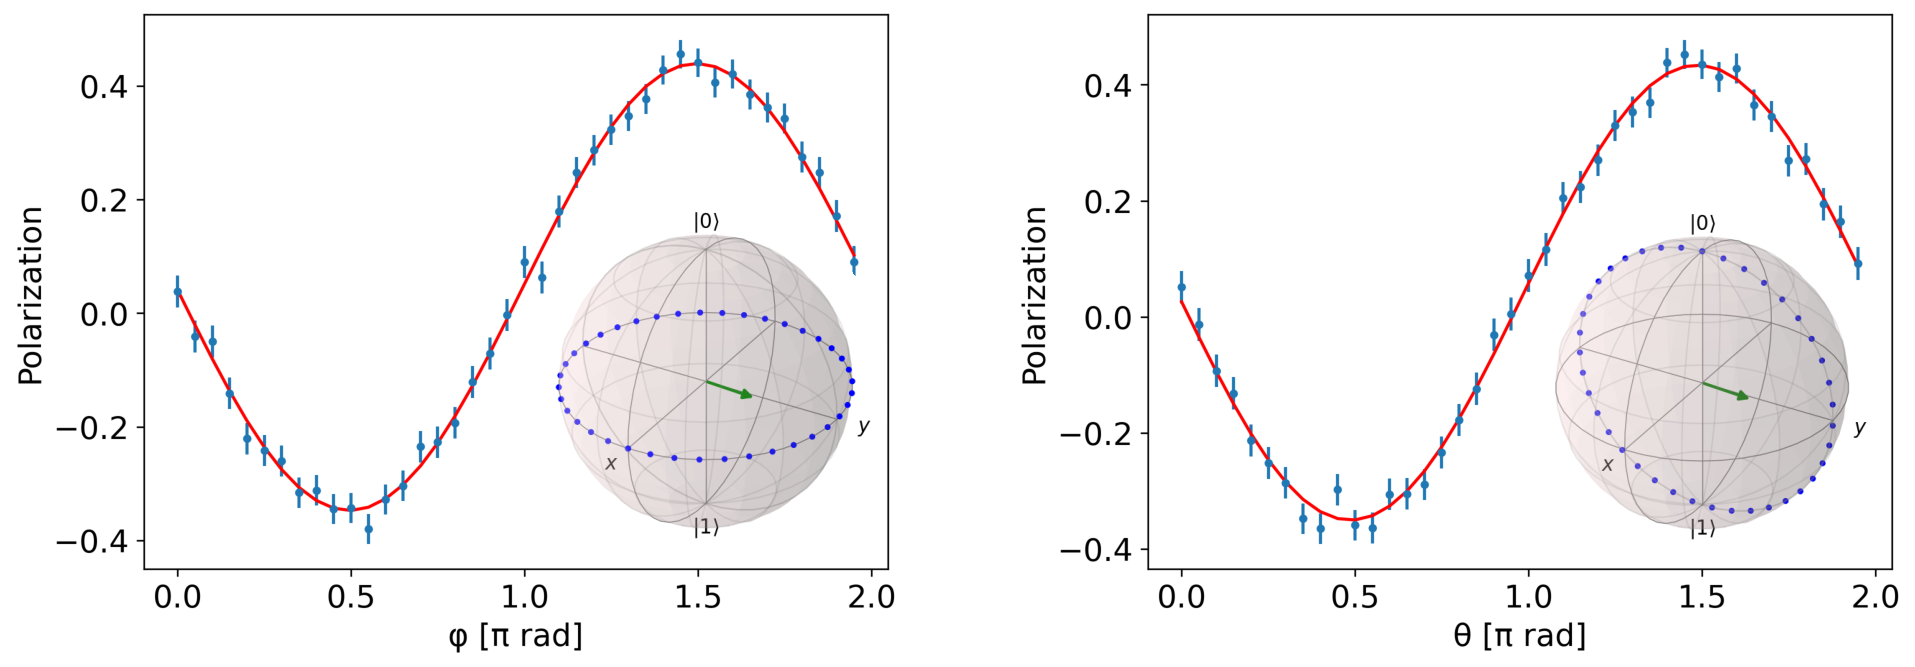
\includegraphics[width=\textwidth]{Figures/t_j_minus.pdf}
    \caption{Numerical simulation of the T-matrix interference protocol and control qubit tomography: The tomography of the control qubit's state after the interference protocol for measuring $T(\tilde{\Phi}_r, \tilde{\Phi}_r) = -i$. The measurement basis was scanned across two planes, see the Bloch sphere diagram (blue dotted circles), and the polarization $P$ was estimated from these measurements, fitting the Eq. \ref{eqn:estim} we have extracted the Bloch vector (orange arrow), from which we have made the estimate: $T(\tilde{\Phi}_r, \tilde{\Phi}_r) = 1.04(1)e^{i\pi 1.496(4)}$. Here the ribbon's path was conditioned, Figure \ref{fig:Tmat}.}
    \label{fig:t_mat_results}
\end{figure*}

In Figures \ref{fig:flav_cond_res} and \ref{fig:ex_cond_res} we have the numerical results of our simulations of the S-matrix interference protocols. We have limited ourselves to a demonstrative selection of cases. Figure \ref{fig:ex_cond_res} shows the results of the protocol in which the existence of the second ribbon is conditioned on the state of the auxiliary qubit, Figure \ref{fig:cond_ex}. The systematic drift of the Bloch vector due to the effects of noise and readout bias are responsible for the underestimate of magnitude of the $\tilde{S}(\Psi_m, \tilde{\Psi}_m)$. Remember that the magnitude of the S-matrix element is dictated by the angle that the Bloch vector makes with respect to the z-axis, not the magnitude of the vector itself which is determined by the effective noise and readout.

The systematic drift is significantly less dramatic in the case of flavour conditioning protocol, Figure \ref{fig:flav_cond_res} for the results and Figure \ref{fig:cond_flav} for the protocol. Hence, the estimate of the magnitudes of the S-matrix elements is much closer to the theoretical value. This is due to the fact that the circuit implementing this protocol is much shallower due to the simpler forms of the conditional ribbon operators, one less Toffoli gate in the conditional multiplication circuit, Figure \ref{fig:flavCond}.

Furthermore, the T-matrix is remarkably well estimated by the path conditioning protocol, Figure \ref{fig:t_mat_results} for the results and Figure \ref{fig:Tmat} for the protocol.

The phases of all values are also estimated remarkably well.

\textbf{Circuit Characteristics.}
In the following text, we report on exact layout used in our simulations of phase sensitive $S-$ and $T-$matrix element measurements.

The exact ribbon operators involved in the protocol are shown in Figure \ref{fig:intef_setup} (Top) while the qubit layout on the Sycamore chip is shown in the bottom of the same Figure.
\begin{figure}
	\centering
	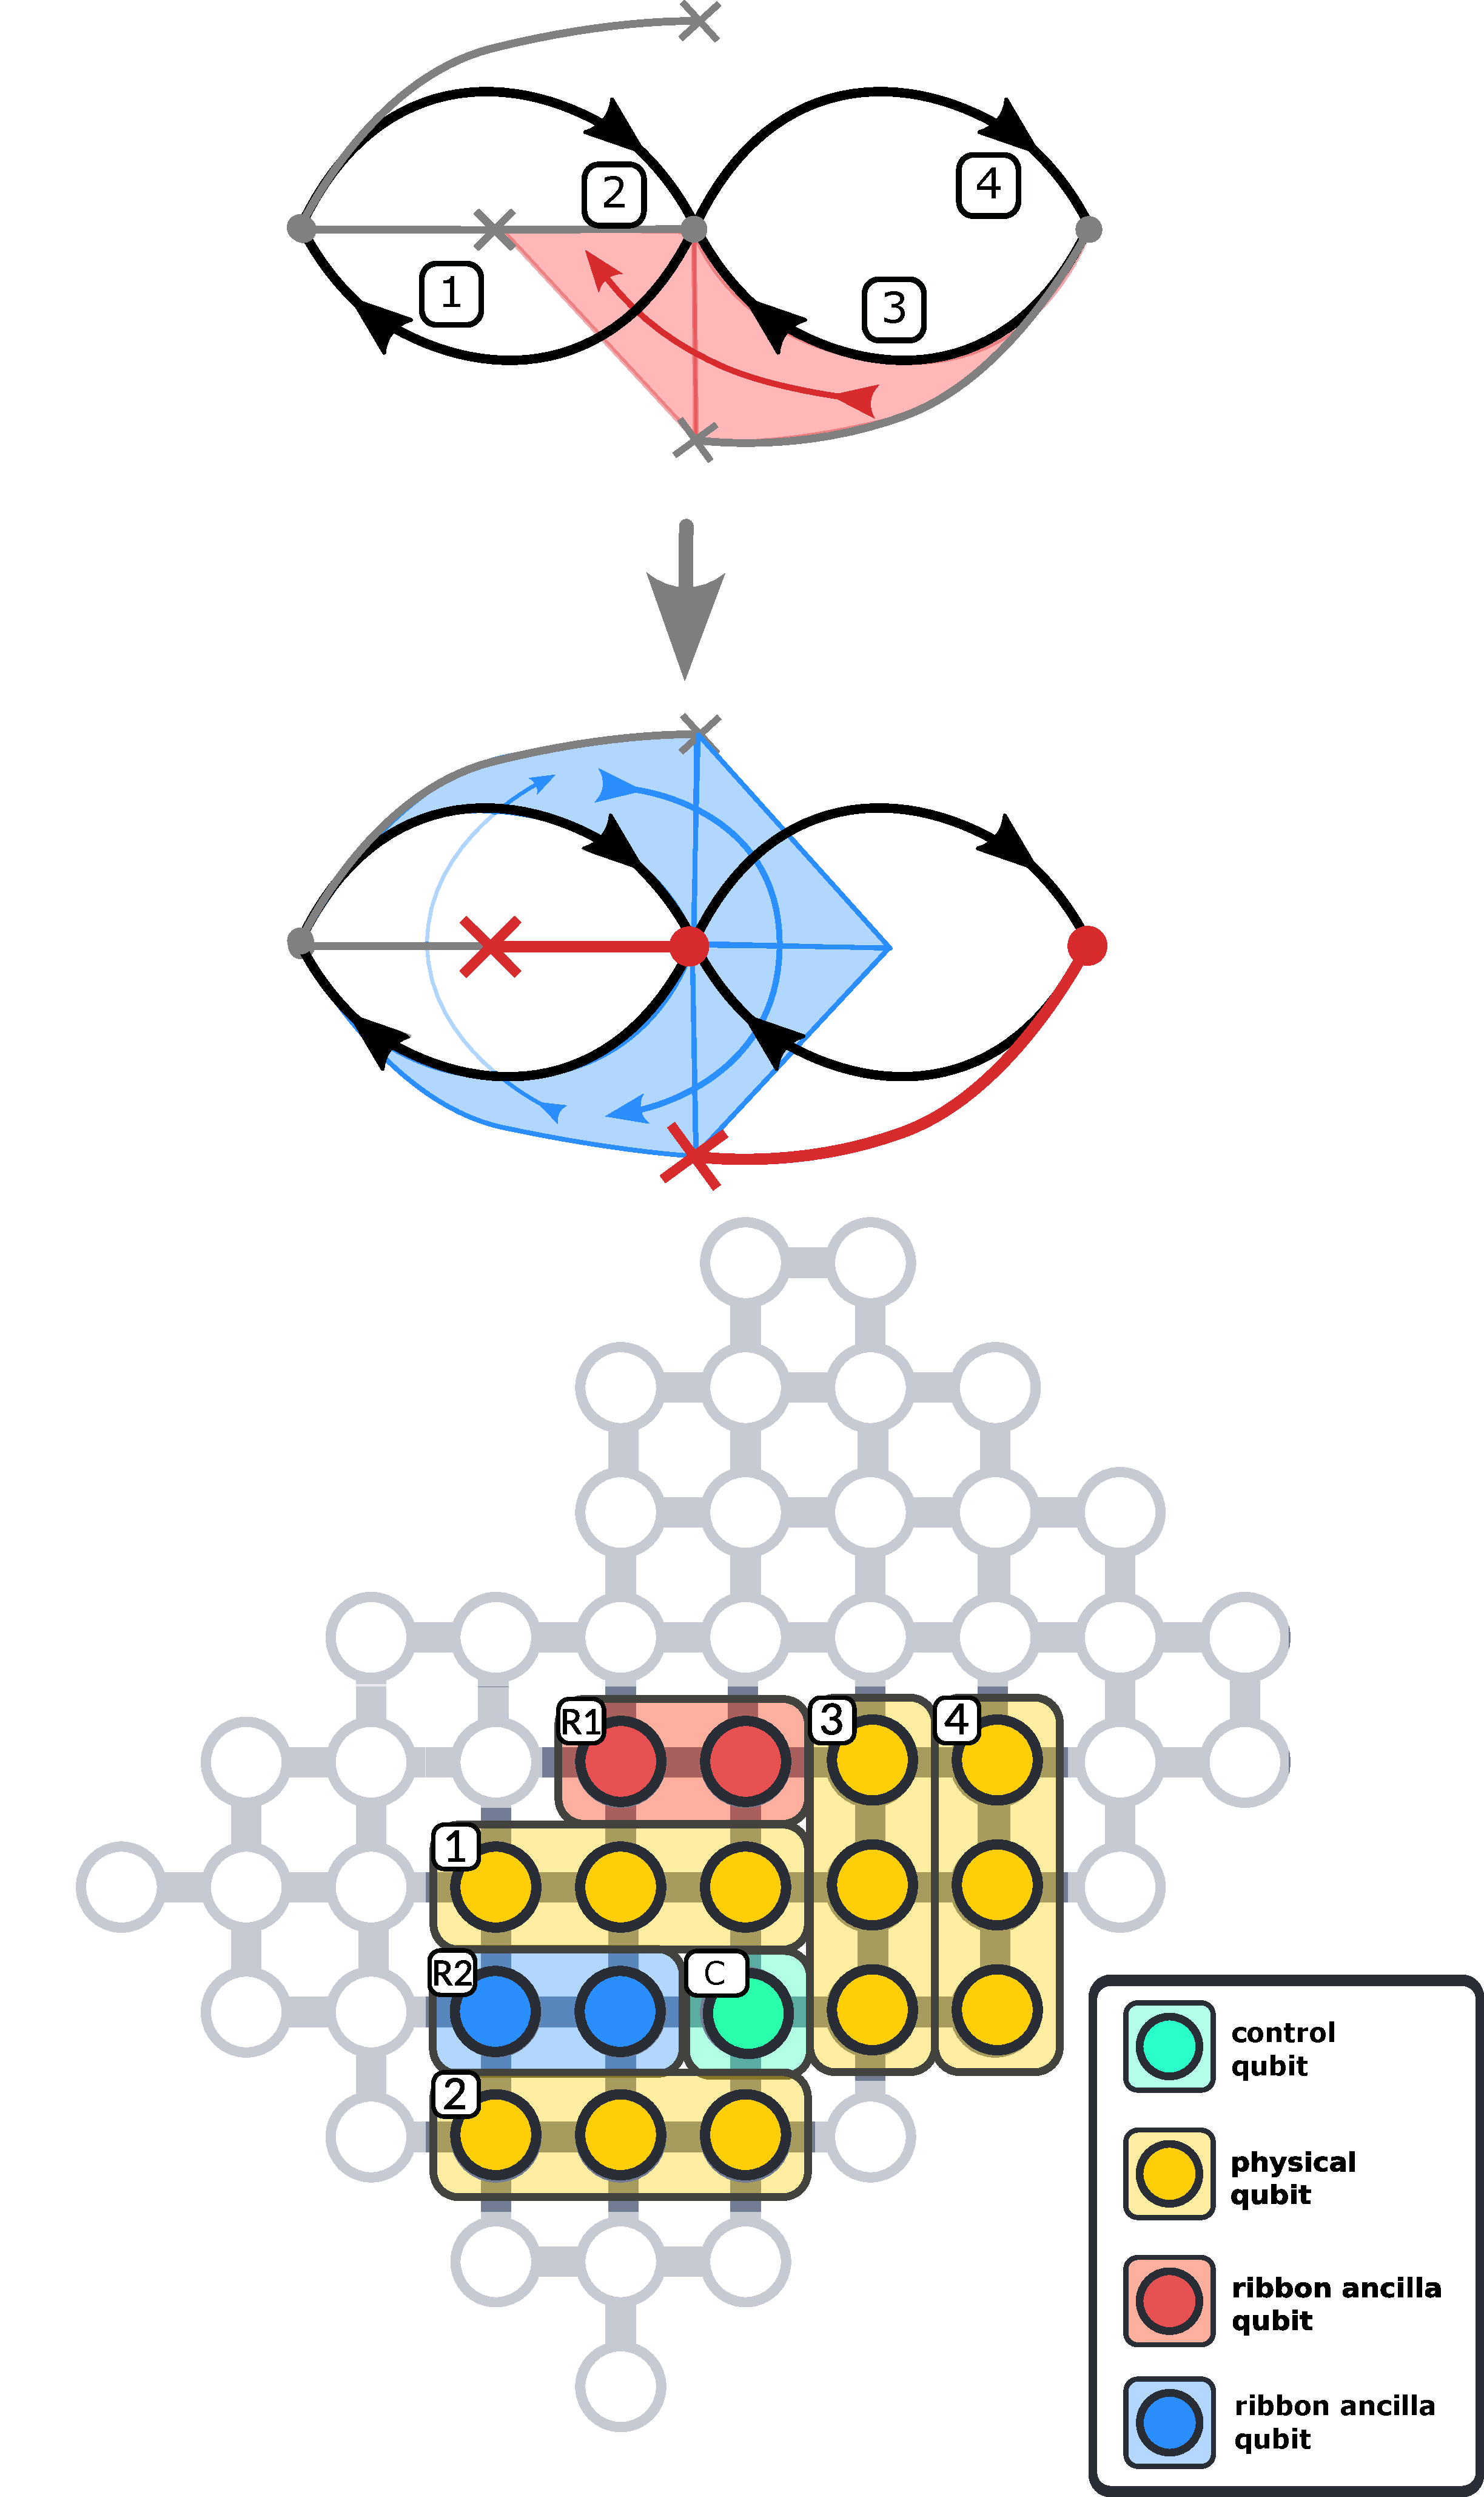
\includegraphics[width=0.75\linewidth]{Figures/intef_setup_new.pdf}
	\caption{(Top) The ribbons operators applied in the simulation. Note that the application or the flavour of the blue (equal-time) ribbon is conditioned on the state of the control bit.  (Bottom) The qubit layout of the interference protocol simulation done via Google Colab platform. The chip simulated is the Google's Sycamore chip and the layout was chosen to occupy a part of the chip with low noise two qubit connections, also this layout reduces the overall number of two qubit gates used int the final circuit.}
	\label{fig:intef_setup}
\end{figure}
Note that the application or the flavour of the blue (equal-time) ribbon is conditioned on the state of the control bit.

The layout on the chip is chosen to reduce the number of two-qubit gates acting on the control bit, which is a more relevant heuristic in this case.

As for the fusion and braiding not all anyons are made equal in term of difficulty to manipulate.

The act of conditioning the application of the ribbon or it's flavour makes this protocol significantly more complex in terms of number of multi-qubit gates.

The two main factors is the flux of the dyon. The $r-$dyons are much more difficult to implement conditionally since they are much more difficult to implement unconditionally. The $\mathbb{Z}_4$ $r$-multiplication necessitates a Toffoli gate upon conditioning.

The second difficulty arrises from the charge. If the irreducible representation of the dyon assigns $-1$ to the nontrivial element of the group's centre, $r^2$, the linear representation formed by $A^{(g)}$ is faithful. Therefore a circuit that implements the generalised conjugation is significantly more complex even before conditioning it.

However, it is important to note that difference in circuits is not  substantial between different types of anyons. The circuit depth are always of the same order of magnitude and involve the same number of qubits. 

With a reasonable improvement in hardware the experiments we propose are doable with all anyons of the $D_4$ theory. 

Given the noise levels present in the simulator we have sticked with using simpler $m$-dyon for most parts. However, the twist phase interferometry experiment we did have to resort to the most complicated anyon, the $\Phi_r$ semion or its antisemion, in order to demonstrate nontrivial twist phase.

The depths of the circuits used in the various interference protocols are:\begin{itemize}
	\item[i)] Flavour conditioning: \begin{enumerate}
		\item[a)] for measuring $S(\Psi_m, \Psi_m)$ and $S(\Psi_m, \tilde{\Psi}_m)$, 58 once completely compiled
		\item[b)] for measuring $S(\Psi_m, \Psi_r)$, 64 once completely compiled, due to the more complex $\mathcal{C}_r$-controlled multiplication
	\end{enumerate}
	
	\item[ii)] Full conditioning will be considerably deeper due to the extra Toffoli gate in conditional $C$-controlled multiplication: \begin{enumerate}
		\item[a)] for measuring $S(\Psi_m, \Psi_m)$ and $S(\Psi_m, \tilde{\Psi}_m)$, 84 once completely compiled
		\item[b)] for measuring $S(\Psi_m, \Psi_r)$, 90 once completely compiled
	\end{enumerate}  
	
	\item[iii)] for measuring $T(\tilde{\Phi}_r, \tilde{\Phi}_r)$, 89 once completely compiled, due to the more complicated $\mathcal{C}_r$-controlled multiplication and generalised conjugation 
\end{itemize}

Note that the twist phase experiment has the best agreement with the theoretical prediction even though it is the deepest protocol.

\emph{Uncertainty.} In the experiment we have used 1000 shots per measurement basis for S-matrix measurements and 5000 for T-matrix measurements.

The uncertainty was estimated by assuming the standard binomial distribution for individual measurement outcome of each shot.

The expected post-selection probability is $1/4$ for all T-matrix protocols and S-matrix protocols with measured $|S| \neq 0$. For the case of measured $|S| = 0$ the probability drops to $1/8$. These probabilities were observed in the numerical experiment.

\section{Other Gauge Groups}\label{sec:other_gauge}

The anyons in the $D_4$ lattice gauge theory are not universal. 
When looking at compiled circuits for our experiments, they are Clifford or close to Clifford circuits.
They are efficiently classically simulatable, given we keep the number of Toffoli gates low.
The image of the braid group onto the transformations of the wavefunction as we braid anyons is finite, hence highly non-universal \cite{}.
This is all due to the simple structure of $D_4$, all of its subgroups are abelian and the group is solvable.
However, if the gauge group in question is $S_3$ for example and if we allow measurements, we achieve computational universality.

In this section, we will discuss what carries over from our study further onto the case of the general group $G$ and in particular $S_3$

\jovan{ToDo.}



\section{Conclusions and Outlook} \label{sec:outlook}

\jovan{Start after the main text.}

%\usepackage[style=phys]{biblatex}


%\bibliographystyle{unsrt}
%\printbibliography
\bibliographystyle{quantum}
\bibliography{bibliography}


\FloatBarrier
\onecolumn
\appendix

\section{Ribbon Types}\label{app:ribs}


In this appendix, we will all the variants of the ribbon operator application algorithm introduced in Section \ref{sec:ribbon_ops}.

More precisely it is how we couple the ancillary qudit with the gauge field degrees of freedom that depending on the exact type of the elementary triangle that is the source of the great number of variants of the application algorithm. 

In the main text we have chosen one case to showcase for the sake of brevity, while in this section we provide an exhaustive list of all sixteen variants.

There are sixteen kinds of elementary triangles, which can be understood as coming from four binary descriptors: the main type of the elementary triangle, is the triangle appended to the frontend or the backend of the ribbon, which of the two orientation the edge of the triangle is in, and the handedness of the triangle. The triangle and its mirror image act as inverses of one another.

The various different rules for the sixteen cases are shown in Figure \ref{fig:al_trigs}. The main actions are controlled multiplication $U_{CM}$ that is controlled by the ancillary qudits and done on the gauge fields degrees of freedom and the generalised conjugation $U_{GC}$ that acts conversely, from the gauge filed onto the ancillary qudits.

Another main distinction is between triangles that are appended to the front and the back of the ribbon, one set involving the forward ancilla, $a_f$, and the other backwards ancilla, $a_b$, respectively. 
\begin{figure}
\centering
\caption*{$U_{CM}\ket{c', i'}_{a_b}\ket{c, i}_{a_f}\ket{g_i}_{\text{phys}} = $}
\vspace{10pt}
	\begin{tabular}{llll}
 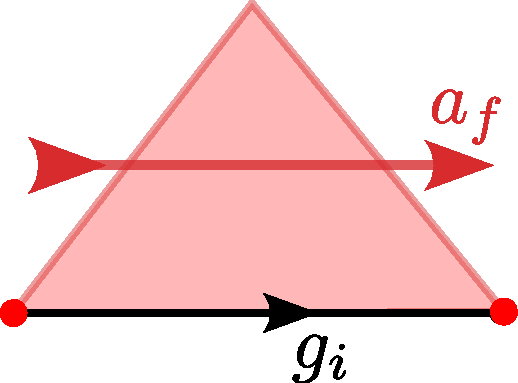
\includegraphics[width=0.12\linewidth]{Figures/IRgf.pdf} &   $\ket{c', i'}_{a_b}\ket{c, i}_{a_f}\ket{cg_i}_{\text{phys}}$ &  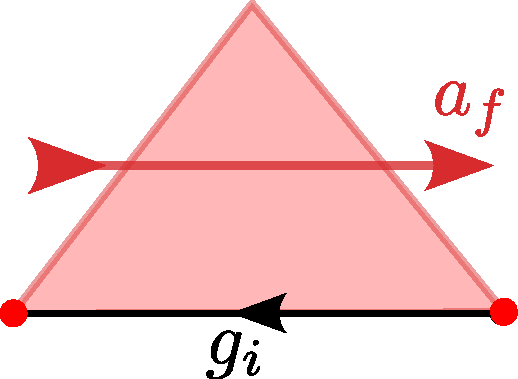
\includegraphics[width=0.12\linewidth]{Figures/IRif.pdf}           &       $\ket{c', i'}_{a_b}\ket{c, i}_{a_f}\ket{g_i c^{-1}}_{\text{phys}}$                  \\ 
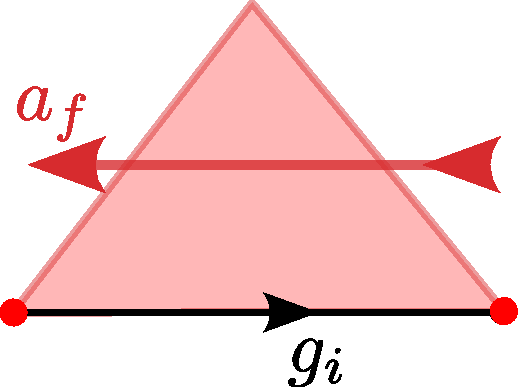
\includegraphics[width=0.12\linewidth]{Figures/ILif.pdf} &   $\ket{c', i'}_{a_b}\ket{c, i}_{a_f}\ket{c^{-1}g_i}_{\text{phys}}$ &  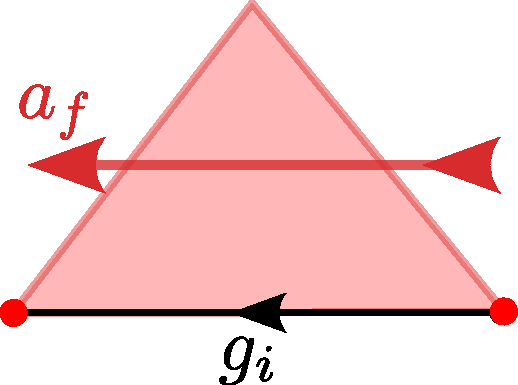
\includegraphics[width=0.12\linewidth]{Figures/ILgf.pdf}           &       $\ket{c', i'}_{a_b}\ket{c, i}_{a_f}\ket{g_i c}_{\text{phys}}$                  \\  
 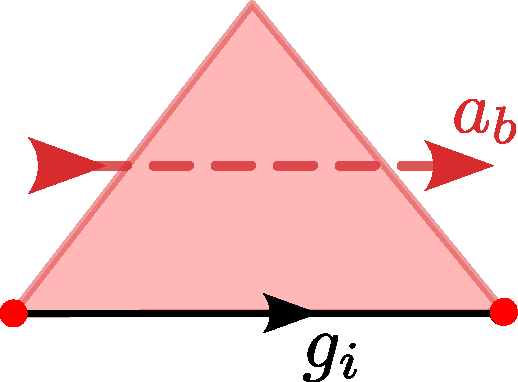
\includegraphics[width=0.12\linewidth]{Figures/IRgb.pdf} &   $\ket{c', i'}_{a_b}\ket{c, i}_{a_f}\ket{c'g_i}_{\text{phys}}$ &  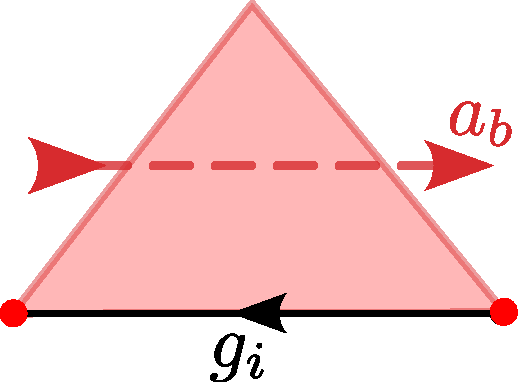
\includegraphics[width=0.12\linewidth]{Figures/IRib.pdf}           &       $\ket{c', i'}_{a_b}\ket{c, i}_{a_f}\ket{g_i c'^{-1}}_{\text{phys}}$                  \\ 
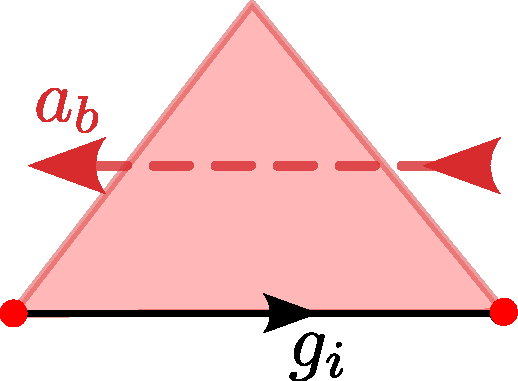
\includegraphics[width=0.12\linewidth]{Figures/ILib.pdf} &   $\ket{c', i'}_{a_b}\ket{c, i}_{a_f}\ket{c'^{-1}g_i}_{\text{phys}}$ &  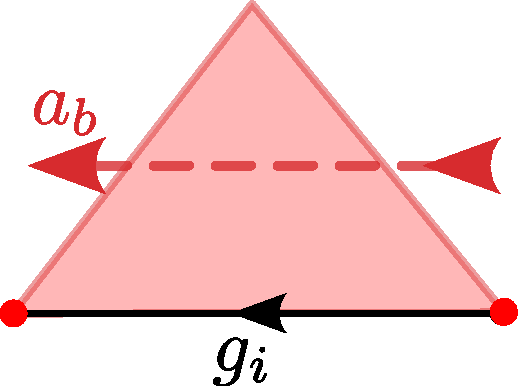
\includegraphics[width=0.12\linewidth]{Figures/ILgb.pdf}           &       $\ket{c', i'}_{a_b}\ket{c, i}_{a_f}\ket{g_i c'}_{\text{phys}}$                  \\  
\end{tabular}\vspace{10pt}

\caption*{$U_{GC}\ket{c', i'}_{a_b} \ket{c, i}_{a_f}\ket{h_i}_{\text{phys}} = $}
\vspace{10pt}
	\begin{tabular}{llll}
 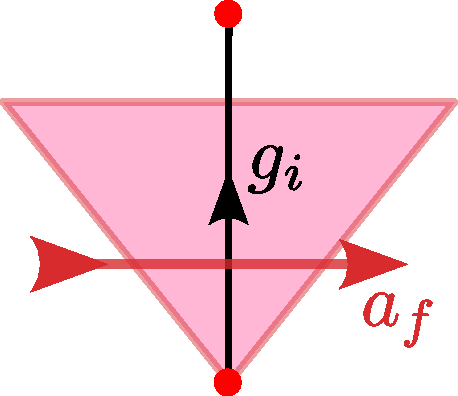
\includegraphics[width=0.12\linewidth]{Figures/IIRgf.pdf} &   $\ket{c', i'}_{a_b}\ket{h_i c h_i^{-1}} \Gamma^{\chi}_c(h_i)\ket{i}_{a_f}\ket{h_i}_{\text{phys}}$ &  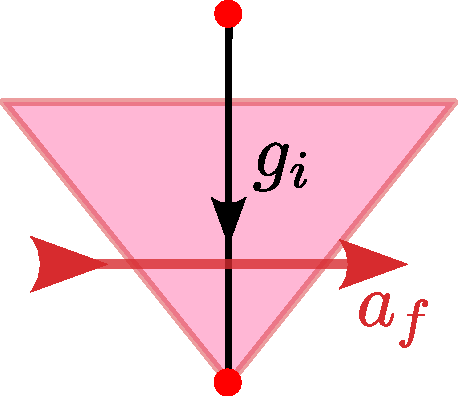
\includegraphics[width=0.12\linewidth]{Figures/IIRif.pdf}           &       $\ket{c', i'}_{a_b}\ket{h_i^{-1} c h_i} \Gamma^{\chi}_c(h_i^{-1})\ket{i}_{a_f}\ket{h_i}_{\text{phys}}$                  \\ 
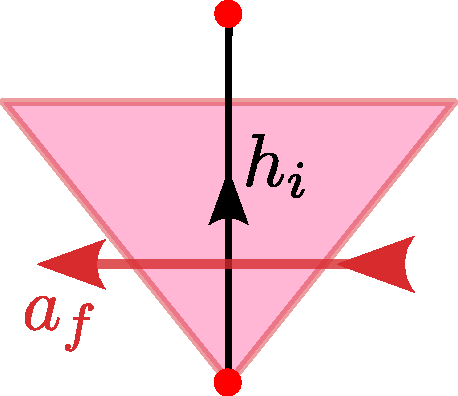
\includegraphics[width=0.12\linewidth]{Figures/IILif.pdf} &   $\ket{c', i'}_{a_b}\ket{h_i^{-1} c h_i} \Gamma^{\chi}_c(h_i^{-1})\ket{i}_{a_f}\ket{h_i}_{\text{phys}}$ &  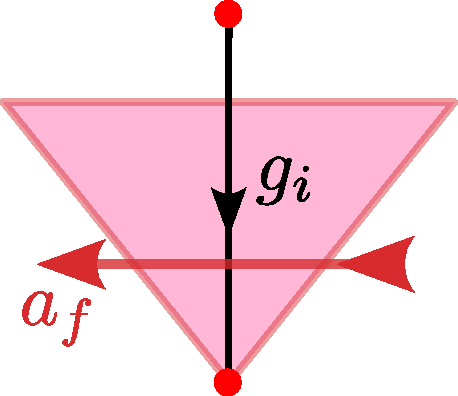
\includegraphics[width=0.12\linewidth]{Figures/IILgf.pdf}           &       $\ket{c', i'}_{a_b}\ket{h_i c h_i^{-1}} \Gamma^{\chi}_c(h_i)\ket{i}_{a_f}\ket{h_i}_{\text{phys}}$                  \\  
 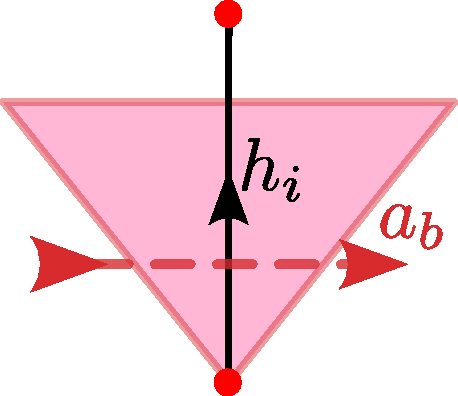
\includegraphics[width=0.12\linewidth]{Figures/IIRgb.pdf} &   $\ket{h_ic'h_i^{-1}}\Gamma_c^{\chi}(h_i)\ket{i'}_{a_b}\ket{c, i}_{a_f}\ket{h_i}_{\text{phys}}$  &  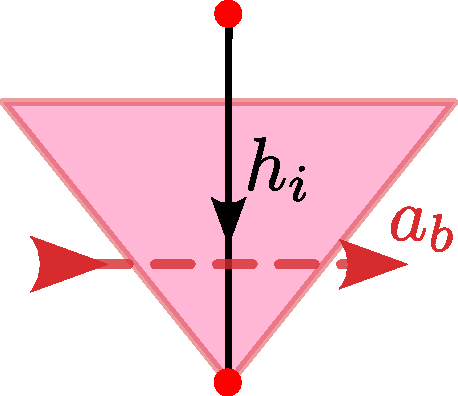
\includegraphics[width=0.12\linewidth]{Figures/IIRib.pdf}           &       $\ket{h_i^{-1}c'h_i}\Gamma_c^{\chi}(h_i^{-1})\ket{i'}_{a_b}\ket{c, i}_{a_f}\ket{h_i}_{\text{phys}}$                  \\ 
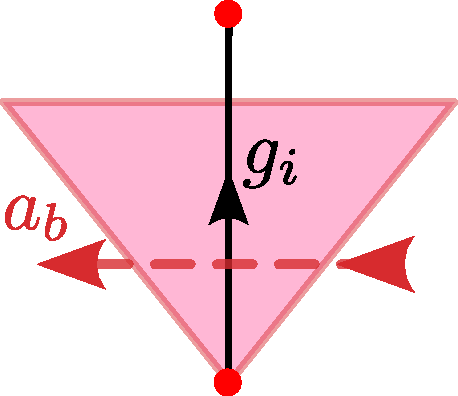
\includegraphics[width=0.12\linewidth]{Figures/IILib.pdf} &   $\ket{h_i^{-1}c'h_i}\Gamma_c^{\chi}(h_i^{-1})\ket{i'}_{a_b}\ket{c, i}_{a_f}\ket{h_i}_{\text{phys}}$ &  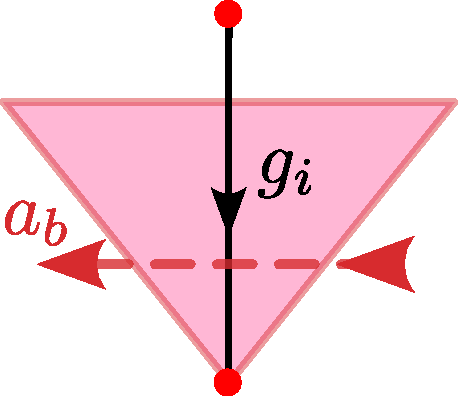
\includegraphics[width=0.12\linewidth]{Figures/IILgb.pdf}           &       $\ket{h_ic'h_i^{-1}}\Gamma_c^{\chi}(h_i)\ket{i'}_{a_b}\ket{c, i}_{a_f}\ket{h_i}_{\text{phys}}$                  \\  
\end{tabular}\vspace{10pt}
\caption{The variants of the ribbon application algorithm for different kinds of Type I and II elementary triangles. \jovan{Type II rules for backwards triangles are wrong because one needs to apply $A^{T}(g)$, which I need to figure out how it is written in our new convention.}}
\label{fig:al_trigs}
\end{figure}
The ability to append to the backend helps in halving the circuit depth of the ribbon application, since, both ends can be grown in parallel, see Figure \ref{fig:both_ends}. In this example the ribbon in Figure \ref{fig:rib_exampl} can be applied in four sequential steps instead of seven if we only grew it by appending the triangles to the frontend.
\begin{figure}
	\centering
	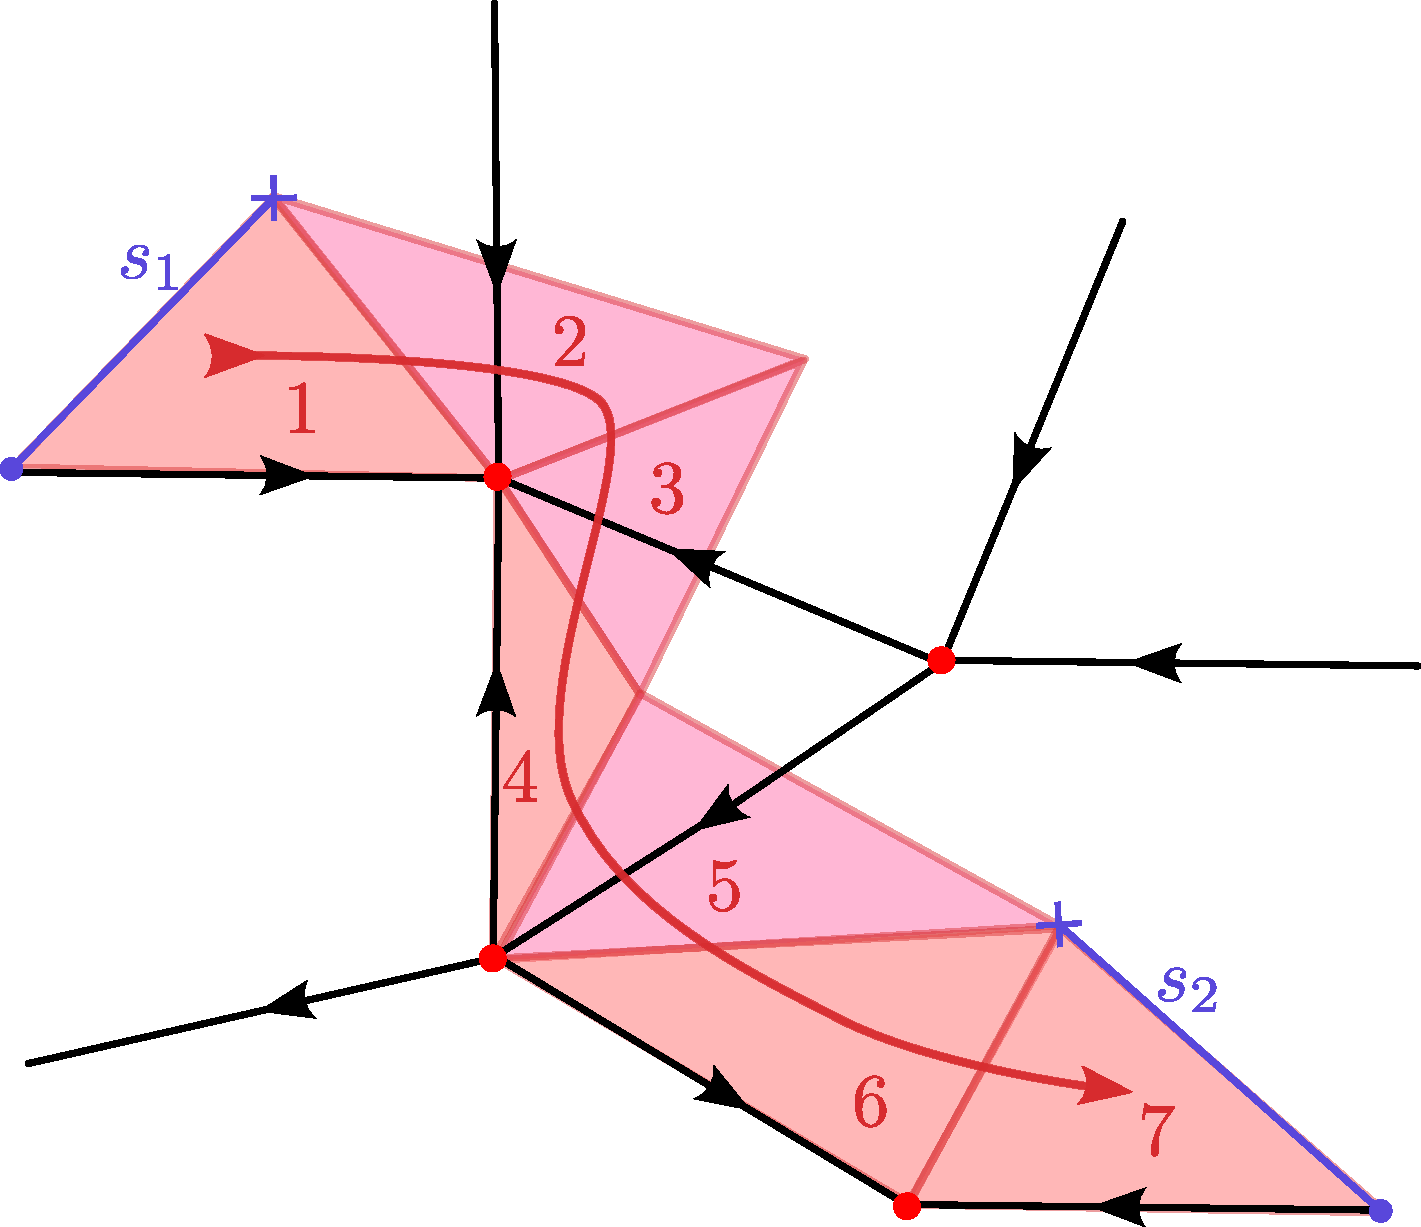
\includegraphics[width=0.45\linewidth]{Figures/front_end.pdf}
	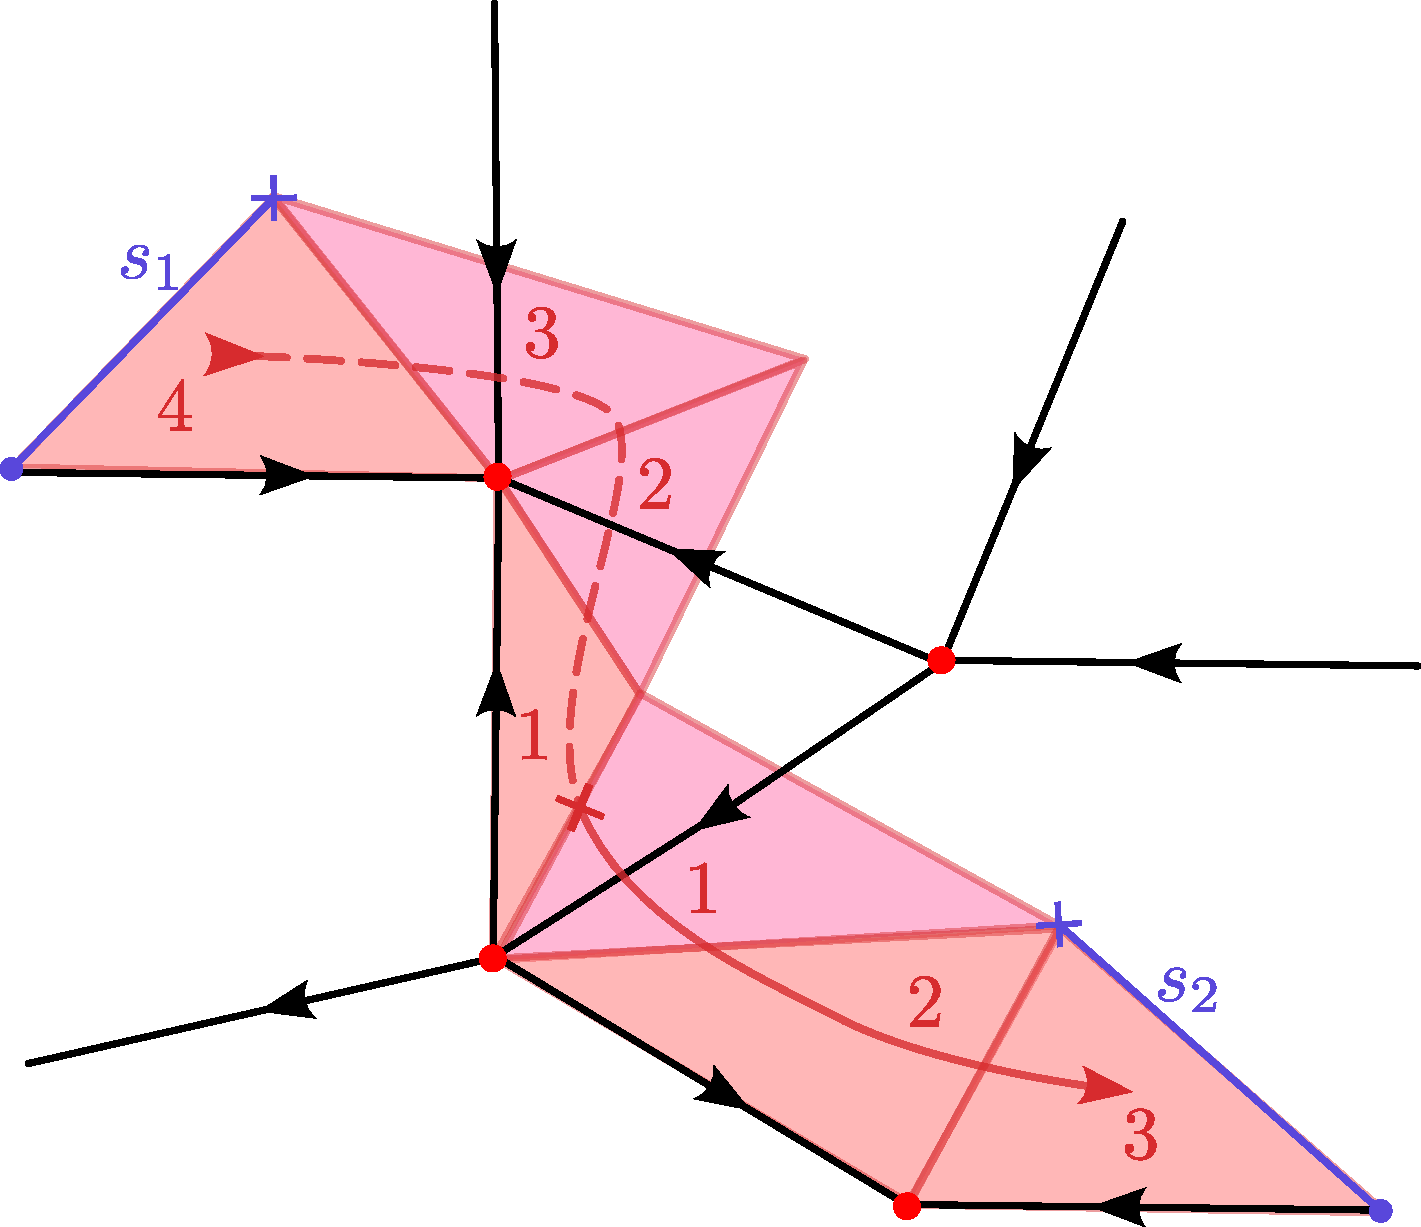
\includegraphics[width=0.45\linewidth]{Figures/both_ends.pdf}
	\caption{The ribbon in Figure \ref{fig:rib_exampl}, broken down so that it can be applied in half the depth, by extending it from the middle ($\times$) in both directions. The numbers label in which layer each elementary triangle can be applied.}
	\label{fig:both_ends}
\end{figure}


\section{Quantum Double Algebra}

\section{Fusion and Braiding of Quantum Double Excitations}\label{app:fusion}\label{app:braid}

\textbf{Fusion.} In section \ref{sec:anyon}, we have mentioned that there is an algebra associated with irreducible representations of the quantum double algebra $D(G)$. In this appendix, we will derive the fusion coefficients that appear in this algebra
\begin{equation}
	a \otimes b = \bigoplus_c N_{ab}^x x,
\end{equation}
where labels $\{a,b,x\}$ are short versions of the full label of the irreducible representations, $x \equiv (C_x, \chi_x)$, where $C_x$ is some conjugacy class of the group $G$ and the $\chi_x$ is a irreducible representation of its centre.

The algebra above is completely analogous to the Clebsch-Gordan decomposition of the product of linear representations of a group into its irreducible representations. The number $N_{ab}^x$ numbers how many time does the representation $x$ appear in the product representations of $a$ and $b$.

To derive this quantity we start with the projector onto the representations $c$
\begin{equation}
	P^x = \frac{\chi_x(e)}{|Z(r_x)|}\sum_{c \in C_x}\sum_{z \in Z(r_x)}\chi_x^*(z)B_x^{(c)}A_x^{(q_c z \bar{q}_c)},
\end{equation}
where $q_c$ is a nonunique group element obeying $q_c c \bar{q}_c = r_x$, with $r_x$ as the $C_x$'s representative.

The matrices $A_x$ and $B_x$ in the equation above are the representation matrices in the $x$ irreducible representations, but the form of the projector is representation independent. We just need to figure out the their form in the $a\otimes b$ representation.

For this specific reason, the quantum double algebra is by definition equiped with a co-product operator
\begin{equation}\begin{split}
	\Delta(A_x^{(g)}) = A_a^{(g)} \otimes A_b^{(g)}\\
	\Delta(B_x^{(h)}) = \sum_{g \in G} B_a^{(g)}\otimes B_b^{(\bar{g}h)}.
\end{split}\end{equation}

After applying the co-product to the $x$-projector we arrive at the form of the projector in the $a\otimes b$ space
\begin{equation}
	P_{a \otimes b}^x = P_{ab}^x = \frac{\chi_x(e)}{|Z(r_x)|}\sum_{c \in C_x}\sum_{z \in Z(r_x)}\sum_{g\in G}\chi_x^*(z)B_a^{(g)}A_a^{(q_c z \bar{q}_c)}\otimes B_b^{(\bar{g}c)}A_b^{(q_c z \bar{q}_c)}.
\end{equation}
 The rank of this projector will be an integer multiple of the dimension of the $x$ representation and that integer is the fusion algebra coefficient $N_{ab}^x$.
 
 The more general way of calculating these fusion coefficients that is more familiar and is applicable for all anyon theories is the Verlinde formula
 \begin{equation}
 	N_{ab}^x = \sum_{l}\frac{S_{al}S_{bl}S^*_{cl}}{S_{0l}},
 \end{equation}
 where the sum is taken over all the anyon labels in the theory, the irreducible representations in our case. The matrix $S$ is the linking matrix and is defined, in terms of the planar diagram algera, as in the diagram in Figure \ref{fig:S_mat_def} (Left).
 \begin{figure}
 	\centering
 	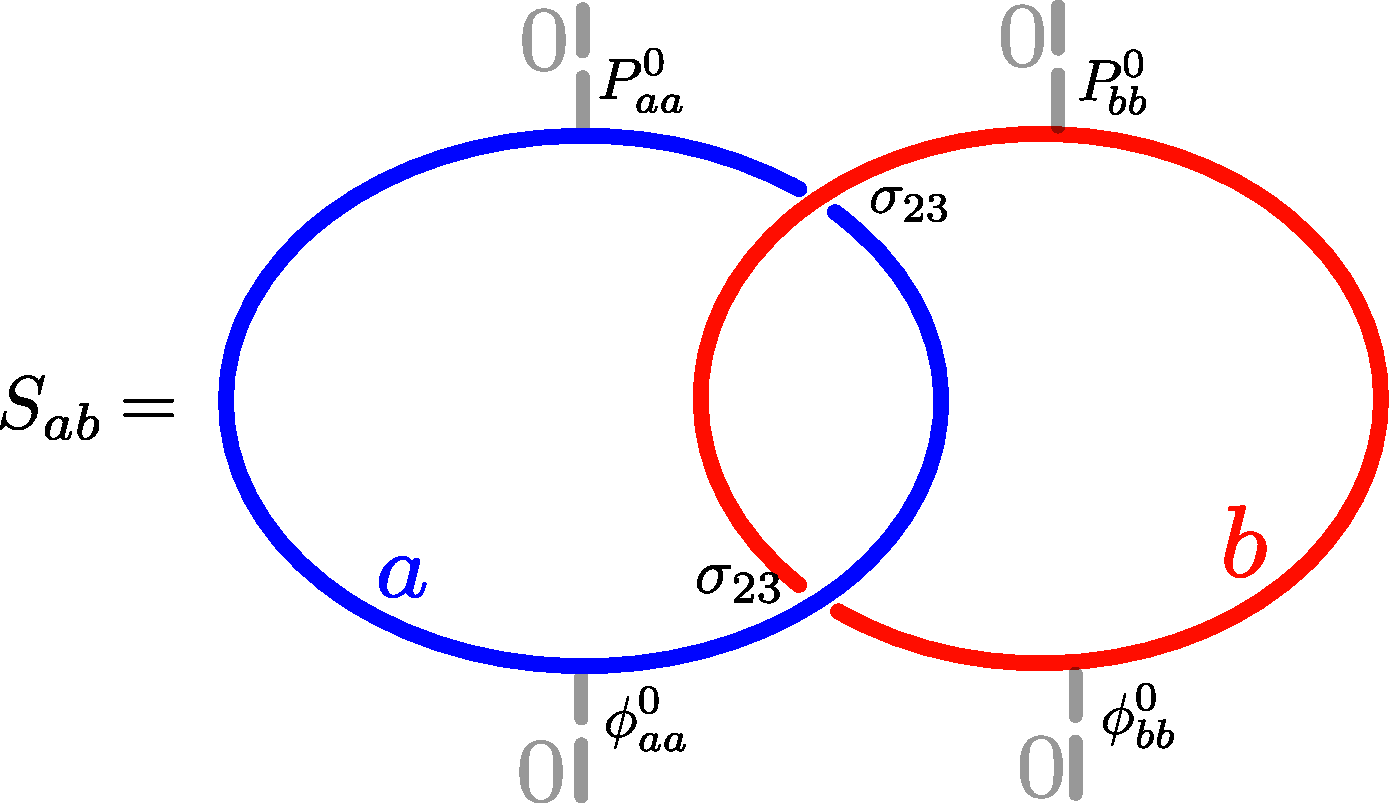
\includegraphics[width= 0.45\linewidth]{Figures/S_mat_def.pdf}\hspace{10pt}
 	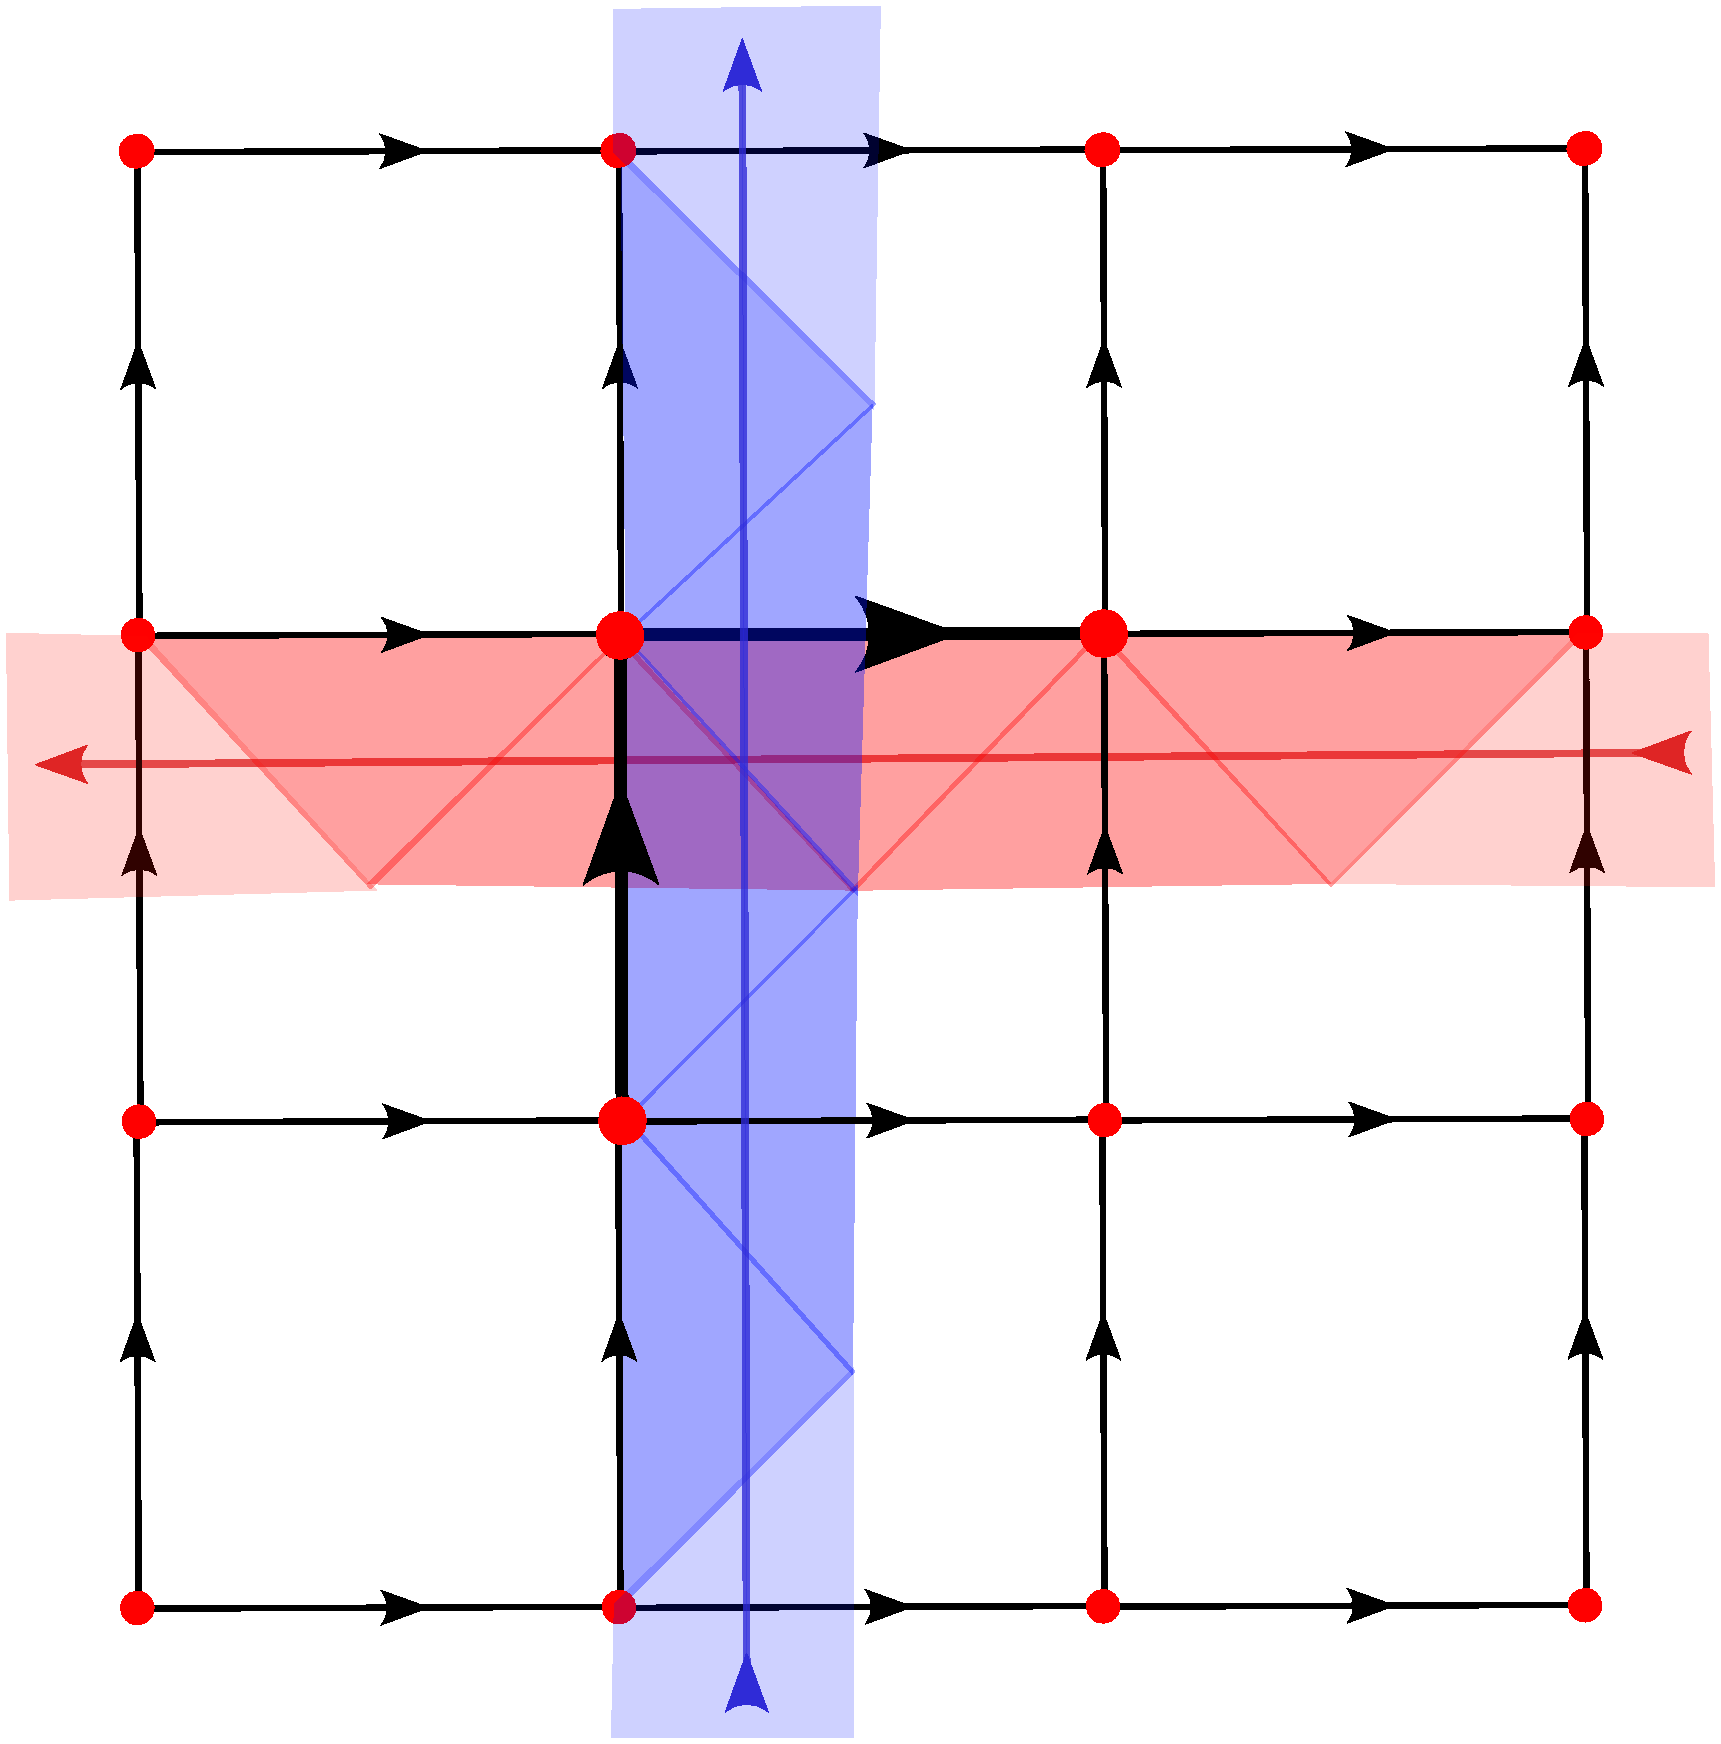
\includegraphics[width= 0.30\linewidth]{Figures/ribbon_crossing.pdf}
 	\caption{(Left) The diagram definition of the linking matrix elements between anyons $a$ and $b$ and its evaluation in the case of the quantum double model. $\sigma_{ii+1}$ represent the action of the braid group generator, the exchange of $i^{\text{th}}$ and $(i+1)^{\text{st}}$ anyon, on the representation space $a \otimes a \otimes b \otimes b$. $P_{xx}^0$ are projectors from the representation space $x \otimes x$ onto the trivial sector and $\phi_{xx}^0$ are functions whose inverses are these projectors. (Right) An example of ribbon crossing that arrises while braiding or annihilating the anyons. The two edges shared between the ribbons are marked in bold. Note that for each edge they share the ribbons have the opposite type of elementary triangle touching it; also that for each ribbon the triangles that touch the two shared edges are of opposite type.}
 	\label{fig:S_mat_def}
 \end{figure}
 
A well known result links the linking matrix of the quantum double model and the representation theory of the gauge group $G$
\begin{equation}
	S_{ab} = \frac{1}{|G|}\sum_{c_a \in C_a, c_b \in C_b, c_a c_b = c_b c_b} \chi_a(q_{c_a}^{-1}c_b q_{c_a})\chi_b(q_{c_b}^{-1}c_a q_{c_b}).\label{eqn:verlinde}
\end{equation}
 
 \textbf{Braiding. }In Figure \ref{fig:S_mat_def} (Left) we also shown how to derive Eq.~\eqref{eqn:verlinde} starting from the quantum double algebra representations, the only additional information we need is also provided by the definition of the quantum double algebra.
The action of the exchange of anyons on the product space is  given by
\begin{equation}
	\begin{split}
		\boldmath{\sigma}_{i i+1}: a_1 \otimes \ldots \otimes a_i \otimes a_{i+1} \otimes \ldots \otimes a_n \rightarrow a_1 \otimes \ldots \otimes a_{i+1} \otimes a_{i} \otimes \ldots \otimes a_n,\\
		\boldmath{\sigma}_{i i+1} = \mathbb{1} \otimes \ldots (\text{Flip } \circ \sum_{h \in G} A_i^{(h)}\otimes B_{i+1}^{(h)}) \otimes \ldots \otimes \mathbb{1},
	\end{split}
\end{equation}
with Flip operator denoting the trivial exchange of vector spaced in the tensor product. One can easily check that the exchange operators defined on this space obey the group multiplication rule of the braid group generators
$$\sigma_{i,i+1}\sigma_{i+1,i+2}\sigma_{i, i+1} =\sigma_{i+1,i+2}\sigma_{i,i+1}\sigma_{i+1, i+2}, $$
hence, it is a representation of the braid group on the product space.

Note that when we do the exchange of actual anyons in our system with the ribbon operators defined in Section \ref{sec:ribbon_ops} this action of the braid group generator is implemented.
The key is that once we perform the braiding (create, exchange and annihilate the anyons) the ribbons of the two exchanged anyons will cross, see Figure \ref{fig:S_mat_def} (Right).
The crossing ribbons share two edges and on these two edges the types of their elementary triangles are opposite, furthermore, the looking at each ribbon individually the the two elementary triangles touching the two edges are also opposite. This remains true even for irregular graphs.

The consequence of this geometrical fact on our protocol is that once the first ribbon traverses the shared edges it will multiply its edge label by it's own flux. And when the second ribbon crosses the edge that the first have had traversed the group action on the auxiliary qudit is shifter by this flux compared to the case where it was traversing the vacuum. This is exactly the required braiding action on the internal space of the anyons
\begin{equation}
	\sigma_{i,i+1}\ket{c, i}_i\ket{c', i'}_{i+1} = \sum_{h \in G}B_{i+1}^{(h)}\ket{c',i'}_{i+1} A_i^{(h)}\ket{c,i}_i = \ket{c',i'}_{i+1} A_i^{(c')}\ket{c,i}_{i}. 
\end{equation}

\section{Representation Theory of $D_4$ and $D(D_4)$}\label{app:reps}
\jovan{$\ldots$}

\section{Circuits for $D_4$-related operations}\label{app:cirqs}

\section{abelian anyons of $D_4$ gauge theory}\label{app:abl}

\section{Post-selection probabilities}\label{app:postsel}

\section{Post-sellection and one-qubit marginals}\label{app:marg}


\end{document}
